% Here we import all packages and set the document type
\documentclass[12pt,spanish,fleqn,openany,letterpaper,pagesize]{scrbook}

\usepackage[utf8]{inputenc}
\usepackage[spanish]{babel}
\usepackage{fancyhdr}
\usepackage{epsfig}
\usepackage{epic}
\usepackage{eepic}
\usepackage{amsmath}
\usepackage{threeparttable}
\usepackage{amscd}
\usepackage{here}
\usepackage{graphicx}
\usepackage{lscape}
\usepackage{tabularx}
\usepackage{subfigure}
\usepackage{longtable}


\usepackage{rotating} %Para rotar texto, objetos y tablas seite. No se ve en DVI solo en PS. Seite 328 Hundebuch
                        %se usa junto con \rotate, \sidewidestable ....


\renewcommand{\theequation}{\thechapter-\arabic{equation}}
\renewcommand{\thefigure}{\textbf{\thechapter-\arabic{figure}}}
\renewcommand{\thetable}{\textbf{\thechapter-\arabic{table}}}


\pagestyle{fancyplain}%\addtolength{\headwidth}{\marginparwidth}
\textheight22.5cm \topmargin0cm \textwidth16.5cm
\oddsidemargin0.5cm \evensidemargin-0.5cm%
\renewcommand{\chaptermark}[1]{\markboth{\thechapter\; #1}{}}
\renewcommand{\sectionmark}[1]{\markright{\thesection\; #1}}
\lhead[\fancyplain{}{\thepage}]{\fancyplain{}{\rightmark}}
\rhead[\fancyplain{}{\leftmark}]{\fancyplain{}{\thepage}}
\fancyfoot{}
\thispagestyle{fancy}%


\addtolength{\headwidth}{0cm}
\unitlength1mm %Define la unidad LE para Figuras
\mathindent0cm %Define la distancia de las formulas al texto,  fleqn las descentra
\marginparwidth0cm
\parindent0cm %Define la distancia de la primera linea de un parrafo a la margen

%Para tablas,  redefine el backschlash en tablas donde se define la posici\'{o}n del texto en las
%casillas (con \centering \raggedright o \raggedleft)
\newcommand{\PreserveBackslash}[1]{\let\temp=\\#1\let\\=\temp}
\let\PBS=\PreserveBackslash

%Espacio entre lineas
\renewcommand{\baselinestretch}{1.1}

%Neuer Befehl f\"{u}r die Tabelle Eigenschaften der Aktivkohlen
\newcommand{\arr}[1]{\raisebox{1.5ex}[0cm][0cm]{#1}}

%Neue Kommandos
\usepackage{Befehle}


%Trennungsliste
\hyphenation {Reaktor-ab-me-ssun-gen Gas-zu-sa-mmen-set-zung
Raum-gesch-win-dig-keit Durch-fluss Stick-stoff-gemisch
Ad-sorp-tions-tem-pe-ra-tur Klein-schmidt
Kohlen-stoff-Mole-kular-siebe Py-rolysat-aus-beu-te
Trans-port-vor-gan-ge}

%\includeonly{Kap1/Kap1,Kap2/Kap2}
\begin{document}

\pagenumbering{roman}

%\newpage
%\setcounter{page}{1}
\begin{center}
\begin{figure}
\centering%

\epsfig{file=HojaTitulo/logoFAMAF.jpg,scale=0.8}%
\end{figure}
\thispagestyle{empty} \vspace*{0.1cm} \textbf{\huge
Estratificación temporal de Aedes Aegypti basada en herramientas geoespaciales y aprendizaje automático}\\[9.0cm]
\Large\textbf{Juan Manuel Scavuzzo}\\[0.5cm]
\small Universidad Nacional de Córdoba\\
Facultad de Matemática, Astronomía, Física y Computación\\
Córdoba, Argentina\\
2018\\
\end{center}

\newpage{\pagestyle{empty}\cleardoublepage}

\newpage
\begin{center}
\thispagestyle{empty} \vspace*{0cm} \textbf{\huge
Estratificación temporal de Aedes Aegypti basada en herramientas Geoespaciales y Machine Learning}\\[3.0cm]
\Large\textbf{Juan Manuel Scavuzzo}\\[2.0cm]
\small Tesis de grado presentada como requisito parcial para optar al
título de:\\
\textbf{Licenciado en Ciencias de la Computación}\\[2.5cm]
Directores:\\

Mgter. Gonzalo Sebastián Peralta (Licenciado en Cs de la Computación y Magíster en Aplicaciones Espaciales)\\
Dr. Jorge Sánchez (Ingeniero en Electrónica y Doctor en Ciencias de la Ingeniería, Visión por computadoras y reconocimiento de patrones)\\ [3.0cm]

Universidad Nacional de Córdoba\\
Facultad de Matemática, Astronomía, Física y Computación\\
Córdoba, Argentina\\
2018\\\end{center}

\newpage{\pagestyle{empty}\cleardoublepage}

\newpage
\thispagestyle{empty} \textbf{}\normalsize
\\\\\\%
\textbf{(Dedicatoria o un lema)}\\[4.0cm]

\begin{flushright}
\begin{minipage}{8cm}
    \noindent
        \small
        Aca va algun lema o algo asi
        Por ejemplo:\\[1.0cm]
        A mis padres\\[1.0cm]\\
        o\\[1.0cm]
        La preocupaci\'{o}n por el hombre y su destino siempre debe ser el
        inter\'{e}s primordial de todo esfuerzo t\'{e}cnico. Nunca olvides esto
        entre tus diagramas y ecuaciones.\\\\
        Albert Einstein\\
\end{minipage}
\end{flushright}

\newpage{\pagestyle{empty}\cleardoublepage}

\newpage
\thispagestyle{empty} \textbf{}\normalsize
\\\\\\%
\textbf{\LARGE Agradecimientos}
\addcontentsline{toc}{chapter}{\numberline{}Agradecimientos}\\\\
insertar agradecimientos

\newpage{\pagestyle{empty}\cleardoublepage}

\newpage
\textbf{\LARGE Resumen}
\addcontentsline{toc}{chapter}{\numberline{}Resumen}\\\\

\textbf{\small Palabras clave: Computer Science, Machine Learning, Python,
      Landscape Epidemiology, Remote Sensing, Dengue, Zika, Chikungunya, Public Health}.\\
\justifying
  \par El Dengue, Zika y Chikungunya son enfermedades virales cuya vacuna para
    prevención aún no existe y que, en los últimos años, han tenido un incremento
    e impacto en la población de la región argentina y latinoamericana que ha
    sido de gran preocupación para los organismos gubernamentales de salud.

  \par En los últimos años se han generado sistemas de riesgo de transmisión
    de enfermedades virales basados en información de sensores remotos,
    estableciendo relaciones entre las condiciones ambientales de las distintas
    zonas con la abundancia del vector en las mismas. A dicha área de estudio
    se la denomina Epidemiología Panorámica.

 \par En el presente trabajo, por un lado, utilizando técnicas de
    ingeniería del software para extraer los requerimientos y aplicar una metodología
    de desarrollo acorde a las necesidades,
    se implementa un \textit{framework} para la generación de modelos de
    aprendizaje automático (ML) con el objetivo
    de estimar la abundancia de vectores de Dengue, Zika y Chikungunya.
    A su vez, se entrenan y evalúan modelos no lineales que poseen mayor
    capacidad de generalización a la hora de modelar las poblaciones del
    mosquito, en comparación con los modelos que actualmente se utilizan
    para tal fin.

  \par Se presenta, además, un enfoque que resuelve el problema de que
    un modelo entrenado con información de una sola ciudad no es capaz,
    en principio, de estimar correctamente la abudancia en otras zonas del país.
    En este trabajo
    se propone resolver la cuestión a traves de un concepto novedoso en el campo
    de la epidemiología, que establece
    relaciones de ``cercanía``
    entre regiones teniendo en cuenta sus características
    ambientales: la Distancia Ambiental Normalizada.


\renewcommand{\tablename}{\textbf{Tabla}}
\renewcommand{\figurename}{\textbf{Figura}}
\renewcommand{\listtablename}{Lista de Tablas}
\renewcommand{\listfigurename}{Lista de Figuras}
\renewcommand{\contentsname}{Contenido}


%\newcommand{\clearemptydoublepage}{\newpage{\pagestyle{empty}\cleardoublepage}}
\tableofcontents
%\include{Resumen}%\newcommand{\clearemptydoublepage}{\newpage{\pagestyle{empty}\cleardoublepage}}
\pagenumbering{arabic}
\documentclass[12pt,spanish,fleqn,openany,letterpaper,pagesize]{scrbook}

\usepackage[utf8]{inputenc}
\usepackage[spanish]{babel}
\usepackage{fancyhdr}
\usepackage{epsfig}
\usepackage{epic}
\usepackage{eepic}
\usepackage{amsmath}
\usepackage{threeparttable}
\usepackage{amscd}
\usepackage{here}
\usepackage{graphicx}
\usepackage{lscape}
\usepackage{tabularx}
\usepackage{subfigure}
\usepackage{longtable}


\usepackage{rotating} %Para rotar texto, objetos y tablas seite. No se ve en DVI solo en PS. Seite 328 Hundebuch
                        %se usa junto con \rotate, \sidewidestable ....


\renewcommand{\theequation}{\thechapter-\arabic{equation}}
\renewcommand{\thefigure}{\textbf{\thechapter-\arabic{figure}}}
\renewcommand{\thetable}{\textbf{\thechapter-\arabic{table}}}


\pagestyle{fancyplain}%\addtolength{\headwidth}{\marginparwidth}
\textheight22.5cm \topmargin0cm \textwidth16.5cm
\oddsidemargin0.5cm \evensidemargin-0.5cm%
\renewcommand{\chaptermark}[1]{\markboth{\thechapter\; #1}{}}
\renewcommand{\sectionmark}[1]{\markright{\thesection\; #1}}
\lhead[\fancyplain{}{\thepage}]{\fancyplain{}{\rightmark}}
\rhead[\fancyplain{}{\leftmark}]{\fancyplain{}{\thepage}}
\fancyfoot{}
\thispagestyle{fancy}%


\addtolength{\headwidth}{0cm}
\unitlength1mm %Define la unidad LE para Figuras
\mathindent0cm %Define la distancia de las formulas al texto,  fleqn las descentra
\marginparwidth0cm
\parindent0cm %Define la distancia de la primera linea de un parrafo a la margen

%Para tablas,  redefine el backschlash en tablas donde se define la posici\'{o}n del texto en las
%casillas (con \centering \raggedright o \raggedleft)
\newcommand{\PreserveBackslash}[1]{\let\temp=\\#1\let\\=\temp}
\let\PBS=\PreserveBackslash

%Espacio entre lineas
\renewcommand{\baselinestretch}{1.1}

%Neuer Befehl f\"{u}r die Tabelle Eigenschaften der Aktivkohlen
\newcommand{\arr}[1]{\raisebox{1.5ex}[0cm][0cm]{#1}}

%Neue Kommandos
\usepackage{Befehle}


%Trennungsliste
\hyphenation {Reaktor-ab-me-ssun-gen Gas-zu-sa-mmen-set-zung
Raum-gesch-win-dig-keit Durch-fluss Stick-stoff-gemisch
Ad-sorp-tions-tem-pe-ra-tur Klein-schmidt
Kohlen-stoff-Mole-kular-siebe Py-rolysat-aus-beu-te
Trans-port-vor-gan-ge}


\begin{document}

\chapter{Motivación}

\justifying
\par El mosquito es uno de los vectores de enfermedades humanas más importantes
  en el mundo. En particular, el \textit{Aedes aegypti} es el principal vector
  de Dengue, Chikungunya, Zika y Fiebre Amarilla urbana [1].
  Según datos de la Organización Mundial de la Salud (OMS), alrededor de 80 millones de
  personas se infectan de Dengue anualmente, cerca de 550 mil enfermos requieren hospitalización y
  unos 20 mil mueren. Además, calculan que más de 2.500 millones de personas corren
  riesgo de contraer la enfermedad y más de 100 países tienen transmisión endémica.
  [Directrices para la prevención y control de Aedes aegypti, está el pdf]
  Algo que cabe aclarar es que en el caso de la Fiebre Amarilla, para la
  prevencion, existe una vacuna de virus atenuado que se considera eficaz, segura
  y se la utiliza hace más de 60 años para la inmunización activa de niños y
  adultos. No es así el caso del Dengue,
  Chikungunya y Zika, para las cuales no existe tal herramienta de previsión.

\par Si tenemos en cuenta las 4 enfermedades mencionadas en el parrafo anterior,
  en las Américas, entre 1985 y 2012, el 95\% de los casos se concentraron en
  4 países: Perú (54\% de los casos), Bolivia (18\%), Brasil (16\%) y Colombia (7\%).
  Otras naciones de la región que presentan condiciones muy
  favorables para la transimisión son Argentina, Ecuador, Panamá y Venezuela.
  Desde 2000 a 2013, más de 1.100 casos confirmados por laboratorio fueron
  reportados.
  [http://www.mdm.org.ar/prensa/articulo/221/Mdicos-del-Mundo-alerta-sobre-riesgos-de-fiebre-amarilla-en-Brasil-y-escenarios-de-Dengue-Zika-en-Argentina\#.W1yUa6zV-AU.link]

\par En el caso de Argentina, ya para las primeras semanas del 2018, hubo casos confirmados
  de Dengue en Chaco, y durante el 2017, en base a las notificaciones al
  \textbf{Sistema Nacional de Vigilancia de Salud} del Ministerio de Salud de la Nación
  recibidas hasta el 30 de diciembre, se registraron, en el primer semestre del año, brotes de
  Dengue serotipo DEN-1 con 646 casos confirmados en 5 provincias
  (Buenos Aires, Chaco, Corrientes, Formosa y Santa Fe) y 253 casos de enfermedad
  por virus del Zika en 3 provincias (Chaco, Formosa y Salta).
  Desde la emergencia del virus del Zika en nuestro país en el 2016 (Tucumán), y hasta
  la [SE 47 REVISAR] de 2017 se registraron además un total de 7 casos confirmados de
  síndrome congénito asociados a virus del Zika en mujeres embarazadas
  (microcefalia en recién nacidos).

\par El Dr. Gonzalo Basile \footnote{Presidente Honor y Director General para
                 América Latina y Caribe de Médicos del Mundo, e investigador de institutos de
                 investigación en salud pública del Caribe y coordinación regional del Programa
                 de Salud Internacional de CLACSO y de FLACSO República Dominicana}
     se refiere al incremento del riesgo de crecimiento
     en la cantidad de casos positivos en nuestro país, teniendo en cuenta
     el contexto epidemiológico en la región:
\begin{framed}

  Aunque las últimas epidemias del 2009 y 2016 de Dengue en Argentina fueron del
  serotipo DEN1, la circulación viral de los otros serotipos en la región de
  Cono Sur (Brasil, Paraguay y Bolivia) tanto DEN4, DEN2 y DEN3, hace que los
  periodos epidémicos de DEN se puedan modificar. Por otro lado, el escenario de
  Zika Virus es una realidad por su circulación en América Latina y Caribe con
  cuadros clínicos inéspecíficos pero con eventos asociados como el Síndrome de
  Guillaen Barré y microcefalia que implican problemas epidemiológicos
  poblacionales de incidencia como lo demostraron en Brasil, Colombia, Venezuela,
  República Dominicana, entre otros 47 países de la región donde se confirmaron
  casos de transmisión activa vectorial de Zika.
  Si sumamos ahora el brote epidémico de Fiebre Amarilla en Brasil con la
  posibilidad de reintroducir casos en el Cono Sur ya que las tasas de
  inmunizaciones para fiebre amarrilla existen brechas en varias ciudades de nuestro país \\

 \centering 24/01/2018
\end{framed}



\par Sumado a lo comentado, por su parte, el \textit{Aedes aegypti} se
  caracteriza por su presencia en el medio urbano, su preferencia
  de cría en contenedores artificiales [3] y la resistencia de sus huevos a la
  desecación. En nuestro país, además, los vertiginosos cambios demográficos, han dado
  por resultado una gran ampliación desorganizada de las zonas urbanas. Ésto, junto
  con el aumento del uso de recipientes no biodegradables y un método deficiente
  de recolección de residuos sólidos, incrementan el número de depósitos que
  acumulan agua, que actúan como potenciales criaderos del mosquito, lo cual aumenta el
  riesgo de ocurrencia de casos de las enfermedades mencionadas.
  Dado que la cantidad de vectores, el virus circulante y la susceptibilidad
  humana dependen directa o indirectamente de variables climáticas y ambientales [buscar cita]
  tales como la temperatura, la lluvia, la vegetación, entre otras, es razonable
  suponer que el cambio climático es, también, un factor de riesgo para el desarrollo
  de las enfermedades en cuestión. Por otra parte, se le suma la capacidad adaptativa del
  \textit{Aedes aegypti} y la aparición de resistencia del mismo debido al uso intensivo de
  insecticidas.


\par Por otro lado, como mencionamos anteriormente, dado que no hay vacunas para la
  mayoría de estos virus, y existe la posibilidad de introducción de otros [2],
  el control de vectores es la principal herramienta para mitigar la
  propagación de enfermedades.


\par Es claro que el escenario epidémico planteado es una realidad en Argentina
  que hay que atacar. Ésto deriva en la necesidad de enfocar esfuerzos en el
  desarrollo de estrategias contundentes dirigidas a evitar, limitar y controlar
  las poblaciones de \textit{Aedes aegyti}, lo que implica repensar y diseñar
  nuevos sistemas de alerta temprana, vigilancia epidemiológica y respuesta
  rápida desde lo local, integrando un espacio interinstitutional e
  intersectorial de coordinación, planificación e intervención pública. Ésto debe
  llevarse a cabo entre el Estado Nacional, municipios, universidades y centros
  de estudio, organizaciones civiles, entre otros actores sociales de gran importancia.
  En ese contexto, la introducción de herramientas científico/tecnológicas orientadas
  a contribuir en esos aspectos resulta fundamental.

\par El uso de información satelital, como uno de los métodos para atacar el
  problema mencionado, se ha estado utilizando desde hace algunos años [cita].
  Ésta técnica permite modelar la evolución temporal y geográfica de las
  poblaciones del vector utilizando variables ambientales obtenidas de los
  sensores remotos. Aunque hasta ahora, estos trabajos utilizaban fuertes asunciones
  al utilizar modelos lineales para relacionar las distintas variables [citas], y por más
  que los resultados obtenidos hasta el momento han sido bastante
  favorables, es simple notar que éstos se podrían mejorar sin asumir dichas relaciones.
  Una de la maneras de evitarlo es la utilización de modelos no-lineales de
  Aprendizaje Automático.

\par Desarrollar un Modelo de Aprendizaje Automático puede resultar extremadamente
  complejo y costoso en términos computacionales y de experiencia de quien lo lleve
  a cabo. Pero uno de los objetivos de este trabajo es mostrar la accesibilidad,
  en términos de simpleza y costos, de algunas de estas herramientas, sin dejar
  de lado el desempeño en la tarea concreta. A su vez, también existe el importante problema
  de la escases de datos de campo para utilizarlos en la construcción de los modelos.
  Hasta ahora, era un gran limitante ya que no se tienen datos vitales
  para el desarrollo de este tipo de herramientas. En este trabajo, además, se
  propone una técnica para atenuar dicho problema estableciendo una relación
  entre los distintos puntos geográficos, en función de sus características ambientales.


  ------------ ACA ESTABA ----------------------------------


el Aprendizaje
Automático es un enfoque que se está utilizando

En ese marco, es que se realiza este trabajo: intentando brindar herramientas
que sean de utilidad, como un aporte de información más, a la hora de tomar
decisiones que respecten al control de estas enfermedades. [5], [6]





En la actualidad el dengue es uno de los principales problemas de salud pública en el mundo.
La  Organización  Mundial  de  la  Salud  (OMS)  estima  que  80  millones  de  personas  se  infectan
anualmente,  y  cerca  de  550  mil  enfermos  necesitan  de  hospitalización,  20  mil  mueren  como
consecuencia de dengue, más de 2.500 millones de personas en riesgo de contraer la enfermedad
y más de 100 países tienen transmisión endémica. Se estima que para el año 2085 el cam-
bio climático pondrá a 3.500 millones de personas en riesgo.


En  el  año  2008  se  observó  una  tendencia  ascendente  de  las  formas  graves  de  dengue.  A  fi-
nales  de  2008  en  los  países  americanos  se  han  registrado  854,134  casos,  con  38,627  dengue
DH,SSD,DCC y 584 muertes (tasa de letalidad de 1,5\%). Durante el  primer semestre del presente
año, se han reportado 571,224 casos de dengue, 10,111 casos de dengue hemorrágico y 200
fallecidos con una tasa de letalidad de 1,98\%. La presencia de los 4 serotipos del dengue (DEN
1,2,3,4) circulando en el continente, elevan el riesgo de las formas graves del dengue.


Los grandes cambios demográficos, que han dado por resultado una gran ampliación desorganizada
de las zonas urbanas, junto con el aumento del uso de recipientes no biodegradables
y un método deficitario de recolección de residuos sólidos, incrementan el número de recipien-
tes que acumulan agua, y que actúan como criaderos potenciales del vector, lo cual aumenta el
riesgo de ocurrencia de casos de dengue.


Por  otro  lado,  la  gran  capacidad  adaptativa  del  vector,  el  uso  intensivo  de  insecticidas  con  la
consecuente aparición de resistencia, el cambio climático y la circulación de los cuatro seroti-
pos del virus DEN en las Américas complican día a día la situación



Los fenómenos derivados del calentamiento global conducen a diferentes combinaciones de
cambios  de  temperatura  y  humedad  cuyas  repercusiones  son  heterogéneas  en  la  incidencia
del  dengue  tanto  en  lo  urbano  como  en  lo  rural,  aspectos  que  requieren  mayores  esfuerzos
entre actores sociales nacionales y jurisdiccionales para una mayor gobernabilidad ambiental.
La estacionalidad de la transmisión es un aspecto a considerar teniendo en cuenta que los vec-
tores han desarrollado estrategias para sobrevivir el invierno y en periodos de sequía. Si bien el
clima es un determinante de esa estacionalidad, las condiciones materiales de vida y el  entorno
físico son modificadores importantes del clima a nivel de campo por la variedad de microclimas
que se conforman donde el Aedes aegypti utiliza estrategias para explotar y maximizar las ventajas a su favor


Desde la reintroducción del virus en 1997-98, el dengue avanza sobre la geografía argentina,
presentándose en forma de brotes esporádicos relacionados con la situación epidemiológica
de otros países y restringido a los meses de mayor temperatura.



Hasta  el  año  2008,  cinco  provincias  habían  presentado  casos  de  dengue  autóctonos  con  la
circulación de tres de los cuatro serotipos existentes. Hasta Junio de 2009, la
cantidad de provincias con circulación viral autóctona asciende a 14



Lo mencionado en párrafos anteriores, hace evidente la necesidad de enfocar esfuerzos
en el desarrollo de estrategias contundentes de parte del Estado y las organizaciones
pertinentes dirigidas a evitar, limitar y controlar las poblaciones de \textit{Aedes aegyti}.
En ese marco, es que se realiza este trabajo: intentando brindar herramientas
que sean de utilidad, como un aporte de información más, a la hora de tomar
decisiones que respecten al control de estas enfermedades.

Lo anterior hace prioritario el desarrollo de  estrategias operacionales de campo, estratificadas,
participativas,  complementarias  y  sostenibles  según  grados  de  riesgo  de  transmisión  (condi-
ciones  socio-ambientales,  movilidad  poblacional,  disponibilidad  de  agua,  períodos  del  año,
niveles de infestación, notificaciones, entre otros), para incrementar la eficacia de las interven-
ciones dirigidas a evitar, limitar o controlar las poblaciones de
Aedes aegyti


En  este  escenario  nacional  e  internacional,  se  hace  necesaria  la  participación  multisectorial,
estableciendo unidades  de  apoyo  técnico  y  científico  que  trabajen  bajo
las  premisas de:  Cogestión, Participación Social, Solidaridad y Equidad, conjuntamente con las
acciones de promoción de la salud, prevención y control de estas patologías.


------------------------------------------------------

En Argentina en las semanas del 2018 ya hay casos confirmados de Dengue en Chaco,
y durante el 2017 y en base a las notificaciones al
\textbf{Sistema Nacional de Vigilancia de Salud} del Ministerio de Salud de la Nación
recibidas hasta el 30 de diciembre se registraron en el primer semestre del año brotes de
dengue serotipo DEN-1 con 646 casos confirmados en 5 provincias
(Buenos Aires, Chaco, Corrientes, Formosa y Santa Fe) y 253 casos de enfermedad
por virus del Zika en 3 provincias (Chaco, Formosa y Salta).
Desde la emergencia del virus del Zika en Argentina en el 2016 (Tucumán) y hasta
la SE 47 de 2017 se registraron además un total de 7 casos confirmados de
síndrome congénito asociados a virus del Zika en mujeres embarazadas (microcefalia en recién nacidos).

\par En el caso de la Fiebre Amarilla, para la prevencion, existe una vacuna de
virus atenuado que se considera eficaz, segura y se la utiliza hace más
de 60 años para la inmunización activa de niños y adultos contra la infección
por dicho virus. No es así el caso del Dengue, Chikungunya y Zika, para las
cuales no existe una vacuna para la prevención.


Los mosquitos son los vectores más importantes de enfermedades humanas en el
mundo y, en particular, el Aedes aegypti es el principal vector de dengue,
chikungunya, zika y fiebre amarilla urbana [1]. Como no hay vacunas para la
mayoría de estos virus, y existe la posibilidad de introducción de otros [2],
el control de vectores es la principal herramienta para mitigar la
propagación de enfermedades. La cantidad de vectores, el virus circulante y la
susceptibilidad humana son factores que influyen en la transmisión de estas
enfermedades virales, estos factores poseen una asociación directa o indirecta
con variables climáticas y ambientales tales como la temperatura, la lluvia,
la vegetación, etc. En particular, en Argentina, \textit{Aedes aegypti} es el
mosquito más relevante desde el punto de vista epidemiológico.
Este mosquito se caracteriza por su presencia en el medio urbano, su preferencia
de cría en contenedores artificiales [3] y la resistencia de sus huevos a la
desecación. Para conocer parámetros sobre las distribuciones espaciales y temporales
de \textit{Aedes aegypti}, se utilizan a menudo las Ovitrampas [4].
Estos datos permiten el conocimiento de la actividad del vector, lo cual es importante para determinar cuándo y
dónde aplicar acciones de control más efectivas [5], [6].




En las Américas, entre 1985 y 2012, el 95\% de los casos se concentraron en
4 países: Perú (54\% de los casos), Bolivia (18\%), Brasil (16\%) y Colombia (7\%).
Los otros países en las Américas que presentan condiciones para la transmisión
de fiebre amarilla son Argentina, Ecuador, Guyana, Guyana Francesa, Panamá,
Paraguay, Suriname, Trinidad y Tobago y Venezuela.
Desde 2000 a 2013, más de 1.100 casos confirmados por laboratorio fueron
reportados en las Américas. Brasil y Perú fueron los países que más casos
reportaron. En áreas urbanas, el Aedes aegypti es el mosquito vector de la
fiebre amarilla. La fiebre amarilla selvática es transmitida por los mosquitos
Haemagogus y Sabethes.

La fiebre amarilla se puede prevenir con la vacuna de virus atenuado de fiebre
amarilla, cepa 17D, que se considera eficaz y segura, y se la utiliza hace más
de 60 años para la inmunización activa de niños y adultos contra la infección
por el virus de la fiebre amarilla. Confiere inmunidad duradera, quizá para toda
la vida. No es el caso del Dengue, Zika y Chikungunya, para las cuales no existen
vacunas para el mismo objetivo.


"[...] El escenario epidémico de Arbovirus como Dengue, Zika y Chikungunya es una
realidad epidemiológica que vino para quedarse en Argentina que implica repensar
y diseñar nuevos sistemas de alerta temprana, vigilancia epidemiológica y
respuesta rápida desde lo local que se integren en un espacio intersectorial de
coordinación, planificación e intervención pública nacional entre municipios,
organizaciones de la sociedad civil, universidades y centros de estudios, y
otros actores sociales claves con una necesaria rectoría del
Ministerio de Salud de la Nación y el Consejo Federal de Salud.
Argentina entro a un impasse en este nuevo periodo inter-epidémicos y realmente
sigue sin tener acciones integradas e integrales para el abordaje de las
Enfermedades Transmitidas por Mosquitos (ETM) en el país y se visualizan
cambios en las estrategias y políticas", alerta Medicos del Mundo [citar].



En Argentina en las semanas del 2018 ya hay casos confirmados de Dengue en Chaco,
y durante el 2017 y en base a las notificaciones al
\textbf{Sistema Nacional de Vigilancia de Salud} del MSN recibidas hasta el
30 de diciembre (SE 52) se registraron en el primer semestre del año brotes de
dengue serotipo DEN-1 con 646 casos confirmados en 5 provincias
(Buenos Aires, Chaco, Corrientes, Formosa y Santa Fe) y 253 casos de enfermedad
por virus del Zika en 3 provincias (Chaco, Formosa y Salta).
Desde la emergencia del virus del Zika en Argentina en el 2016 (Tucumán) y hasta
la SE 47 de 2017 se registraron además un total de 7 casos confirmados de
síndrome congénito asociados a virus del Zika en mujeres embarazadas (microcefalia en recién nacidos).



Médicos del Mundo, viene advirtiendo que las acciones implementadas aleatoriamente
de control vectorial y control químico tradicional no son efectivas ni eficaces
para actual contexto epidémico en la región y el país.




"Aunque las últimas epidemias del 2009 y 2016 de Dengue en Argentina fueron del
serotipo DEN1, la circulación viral de los otros serotipos en la región de
Cono Sur (Brasil, Paraguay y Bolivia) tanto DEN4, DEN2 y DEN3, hace que los
periodos epidémicos de DEN se puedan modificar. Por otro lado, el escenario de
Zika Virus es una realidad por su circulación en América Latina y Caribe con
cuadros clínicos inéspecíficos pero con eventos asociados como el Síndrome de
Guillaen Barré y microcefalia que implican problemas epidemiológicos
poblacionales de incidencia como lo demostraron en Brasil, Colombia, Venezuela,
República Dominicana, entre otros 47 países de la región donde se confirmaron
casos de transmisión activa vectorial de Zika.
Si sumamos ahora el brote epidémico de Fiebre Amarilla en Brasil con la
posibilidad de reintroducir casos en el Cono Sur ya que las tasas de
inmunizaciones para fiebre amarrilla existen brechas en varias ciudades de nuestro país",
detalló Gonzalo Basile, Presidente Honor y Director General para
América Latina y Caribe de Médicos del Mundo, e investigador de institutos de
investigación en salud pública del Caribe y coordinación regional del Programa
de Salud Internacional de CLACSO y de FLACSO República Dominicana.





"Desde Médicos del Mundo venimos advirtiendo en lo regional que para el abordaje
de las Arbovirosis hay que repensar nuevos marcos conceptuales y metodológicos
sobre la Salud y la Epidemiología en las Ciudades por el tipo de urbanizaciones
caóticas, inequitativas y con déficit en agua, gestión integral de residuos y
saneamiento ambiental estructurales de enfermedades transmitidas por mosquitos.
Y en segundo lugar, los determinantes vinculados a los patrones climáticos
extremos que generan comportamientos nuevos de los vectores y transmisión de
enfermedades especialmente como Zika, Dengue, Malaria, entre otras.
No es posible continuar haciendo lo mismo que hace 40 años hacemos con Dengue en
la región y esperar resultados diferentes. La transferencia individual de
información y la "responsabilización" individual en los estilos de vida y
comportamientos particulares de las personas está demostrado no son el camino
para enfrentar escenarios epidemiológicos que seguirán complejizándose en el país
y en América Latina y Caribe", concluyó Gonzalo Basile.





Específicamente,

Specifically, in a interinstitutional framework between the Argentinean
National Space Agency (CONAE) and the Health Minister of Argentine,
there have been initiatives to model the temporal evolution of mosquito pop-
ulations using environmental variables obtained from remote sensors. These
works used series of a few years and are based on a small number of satellite
variables [36, 37]. In an effort to improve this, (author?) [38] constructed
models based on a large number of variables from various sensors for four
years. All these works assumed multivariate linear models.
This work represent an improvement of that scenario. We compare Sup-
port Vector Machines, Artificial Neural Networks, K-nearest neighbors and
Decision Tree Regressor in addition to two linear approaches. With this,
we obtain an operational methodology which contributes to the Argentinean
Dengue risk system currently in operation [31, 39].
We explore, in contrast to previous ones, the ability of modeling and
predicting oviposition with out of the shelf ML algorithms, i.e., with min-
imum parameter tuning, as provided by FLOSS – Free/Libre Open Source
Software. This promotes the assimilation of these techniques for the whole
community that deals with similar problems.



--------------------------------







\end{document}

%\documentclass[12pt,spanish,fleqn,openany,letterpaper,pagesize]{scrbook}

\usepackage[utf8]{inputenc}
\usepackage[spanish]{babel}
\usepackage{fancyhdr}
\usepackage{epsfig}
\usepackage{epic}
\usepackage{eepic}
\usepackage{amsmath}
\usepackage{threeparttable}
\usepackage{amscd}
\usepackage{here}
\usepackage{graphicx}
\usepackage{lscape}
\usepackage{tabularx}
\usepackage{subfigure}
\usepackage{longtable}


\usepackage{rotating} %Para rotar texto, objetos y tablas seite. No se ve en DVI solo en PS. Seite 328 Hundebuch
                        %se usa junto con \rotate, \sidewidestable ....


\renewcommand{\theequation}{\thechapter-\arabic{equation}}
\renewcommand{\thefigure}{\textbf{\thechapter-\arabic{figure}}}
\renewcommand{\thetable}{\textbf{\thechapter-\arabic{table}}}


\pagestyle{fancyplain}%\addtolength{\headwidth}{\marginparwidth}
\textheight22.5cm \topmargin0cm \textwidth16.5cm
\oddsidemargin0.5cm \evensidemargin-0.5cm%
\renewcommand{\chaptermark}[1]{\markboth{\thechapter\; #1}{}}
\renewcommand{\sectionmark}[1]{\markright{\thesection\; #1}}
\lhead[\fancyplain{}{\thepage}]{\fancyplain{}{\rightmark}}
\rhead[\fancyplain{}{\leftmark}]{\fancyplain{}{\thepage}}
\fancyfoot{}
\thispagestyle{fancy}%


\addtolength{\headwidth}{0cm}
\unitlength1mm %Define la unidad LE para Figuras
\mathindent0cm %Define la distancia de las formulas al texto,  fleqn las descentra
\marginparwidth0cm
\parindent0cm %Define la distancia de la primera linea de un parrafo a la margen

%Para tablas,  redefine el backschlash en tablas donde se define la posici\'{o}n del texto en las
%casillas (con \centering \raggedright o \raggedleft)
\newcommand{\PreserveBackslash}[1]{\let\temp=\\#1\let\\=\temp}
\let\PBS=\PreserveBackslash

%Espacio entre lineas
\renewcommand{\baselinestretch}{1.1}

%Neuer Befehl f\"{u}r die Tabelle Eigenschaften der Aktivkohlen
\newcommand{\arr}[1]{\raisebox{1.5ex}[0cm][0cm]{#1}}

%Neue Kommandos
\usepackage{Befehle}


%Trennungsliste
\hyphenation {Reaktor-ab-me-ssun-gen Gas-zu-sa-mmen-set-zung
Raum-gesch-win-dig-keit Durch-fluss Stick-stoff-gemisch
Ad-sorp-tions-tem-pe-ra-tur Klein-schmidt
Kohlen-stoff-Mole-kular-siebe Py-rolysat-aus-beu-te
Trans-port-vor-gan-ge}

%
%\begin{document}

\chapter{Marco teórico}

\section{Epidemiología panorámica}

\justifying


\par La \textit{Teledetección} se define como el proceso de adquirir
  información acerca de un objeto, área o fenómeno desde la distancia.
  Un sensor remoto es un instrumento capaz de realizar percepción remota, por lo
  que en esta amplia definición caben desde los ojos hasta los
  radiotelescopios.

\par Existen dos grandes tipos de sensores remotos (SR): activos y pasivos.
  Los activos son aquellos que obtienen la información generando su propia energía
  mientras que los pasivos dependen de una fuente externa, que en la Tierra
  principalmente proviene del Sol. Hasta el día de hoy, los más usados son los
  sensores pasivos dado que permiten medir la magnitud de la radiación electromagnética
  reflejada e irradiada desde la superficie de la Tierra y de la atmósfera y,
  de esta manera, derivar información sobre las condiciones de la superficie \cite{cami_tartagal}.


\par Los SR más utilizados y con mayor cantidad de aplicaciones son los que se
  encuentran a bordo de satélites que orbitan sobre la Tierra, bien sea
  en órbitas geoestacionarias\footnote{Están en altitudes entre 23000 y 40000 km,
  sobre la franja ecuatorial y viajan a la misma velocidad de rotación de la Tierra
  por lo que siempre están fijos sobre un punto determinado de la superficie terrestre.},
  u órbitas polares, aquellas que pasan repetidamente por diferentes áreas
  de la Tierra mientras están orbitando alrededor del planeta a altitudes menores.


\par Las tecnologías relacionadas al ámbito aeroespacial dieron lugar a programas
  que integran estas tecnologías con,
  por ejemplo, la agricultura, salud pública, geología y las ciencias forestales.
  A su vez, la información obtenida por dichos SR se puede aplicar a estudios
  entomológicos\footnote{De insectos.}, debido a que ellos proveen gran cantidad
  y diversidad de información sobre la cobertura de la Tierra: características
  de la vegetación, cuerpos de agua, temperaturas, entre otras. Ésta, también es
  información sobre el hábitat de insectos y artrópodos vectores \cite{ndwi_erffectiveness, data_driven_prediction},
  y, por lo tanto, de acuerdo a la teoría de Pavlovsky \cite{nidality} en la que
  expone la correlación entre el hábitat y enfermedades transmitidas por vectores,
  los datos de los SR se pueden utilizar como fuente de información sobre la
  distribución espacio-temporal de dichas afecciones.


\par Con la acumulación de datos registrados por sensores remotos desde los años
  70 existen series temporales que permiten realizar varios tipos de análisis con
  relevancia para la transmisión de la enfermedad de Dengue y otras
  ETV\footnote{Enfermedades de Transmisión Vectorial.}.
  Entre ellas, series temporales de imágenes de mediana resolución espacial
  permiten analizar en perspectiva histórica los cambios de uso y cobertura del
  terreno, proceso que habitualmente tiene vinculación con cambios en la
  epidemiología de la enfermedad \cite{german_temporal}.
  A su vez, el deterioro de las condiciones de salud en el mundo, el avance significativo
  en el procesamiento de computadoras, la mejora en la adquisición de datos,
  la reducción de los costos de hardware y software y el desarrollo de tecnología
  GIS\footnote{Sistema de Información Geográfica.}(por sus siglas en inglés) han llevado al lanzamiento
  de programas que apuntan a integrar SR / GIS en aplicaciones de salud
  \cite{tesis_riesgo_viral, tesis_gonza, espinosa_temporal, rs_public_health}.



\par El uso de técnicas de Teledetección para mapear la distribución de vectores y el riesgo
  de enfermedades ha tenido una gran evolución durante las últimas dos
  décadas. La complejidad de las técnicas va desde el uso de simples
  correlaciones entre las firmas espectrales de diferentes coberturas, usos del
  suelo y abundancia de especies hasta técnicas complejas que integran variables
  ambientales obtenidas de satélites con la biología de los vectores.
  Estas técnicas se usan para desarrollar modelos predictivos de riesgo,
  los cuales principalmente se realizan a través de técnicas estadísticas de
  regresión logística y análisis discriminante, que dilucidan las asociaciones
  entre datos ambientales multivariados y los patrones de presencia o ausencia de
  vectores para así mapear los vectores o las enfermedades.
  Estos métodos son capaces de predecir la probabilidad “\textit{a posteriori}” de la
  presencia de la variable dependiente (vector o enfermedad), a partir de un
  grupo de variables independientes (datos de clima y cobertura de la tierra) y de esta
  forma pueden ser usados para hacer mapas de riesgo a partir de bases de datos.


% la vision panotamira de los problemas de este tipo esta vinculada con la
% el hecho de que dichos problemas dependen de un entorno no local
\par Las condiciones ambientales que determinan la
  conectividad\footnote{El grado en que el paisaje impide o facilita el movimiento
  entre las zonas de recursos \cite{landscape_connectivity}.} de los paisajes
  para la dispersión pueden variar en las distintas regiones y dependen de cómo
  el patógeno se dispersa biológicamente (ej. dado un patógeno portado por
  vectores, el movimiento del insecto) o abióticamente (e.j: flujos de viento o agua).
  Por ejemplo, rios y corrientes pueden actuar como corredores de dispersión que
  fomentan la propagación de la infección a través de paisajes heterogéneos
  para patógenos de plantas transmitidos por el agua. En otros
  sistemas, como las enfermedades zoonóticas de mamíferos terrestres, estos mismos
  cuerpos de agua pueden funcionar como barreras impidiendo el movimiento
  del huésped o del vector. Estas condiciones se ven reflejadas en la
  Figura \ref{fig:paisajes_h} de \cite{landscape_epidemiology}.
  Notemos que en el caso de \textbf{a)}, la
  conectividad entre los sitios azules es mayor que la que se da entre éstos y
  los amarillos, y también entre ellos y los rojos, siendo que la distancia
  euclídea entre los azules es mayor. Ésto ocurre porque el sitio rojo está del otro lado
  de la cordillera, la cual funciona como una barrera geográfica para la
  inoculación\footnote{Introducción de microorganismos vivos, muertos o atenuados,
  en un organismo de forma accidental o voluntaria.}, el huésped y/o la dispersión
  del vector. En el caso \textbf{b)}, en cambio, se da la situación de un
  patosistema\footnote{Subsistema dentro del sistema agrícola caracterizado por el
  fenómeno de parasitismo. Está constituido por un hospedante susceptible,
  un patógeno virulento y un ambiente predispuesto a la enfermedad.} acuático, en
  donde la inoculación sucede a través del agua: los dos sitios amarillos son los
  más estrechamente conectados, a pesar de que están separados por una mayor
  distancia euclídea que con otros, porque el sitio amarillo de abajo está localizado
  bajo una corriente que va desde el sitio amarillo de arriba.


    \begin{figure}
    \centering%
    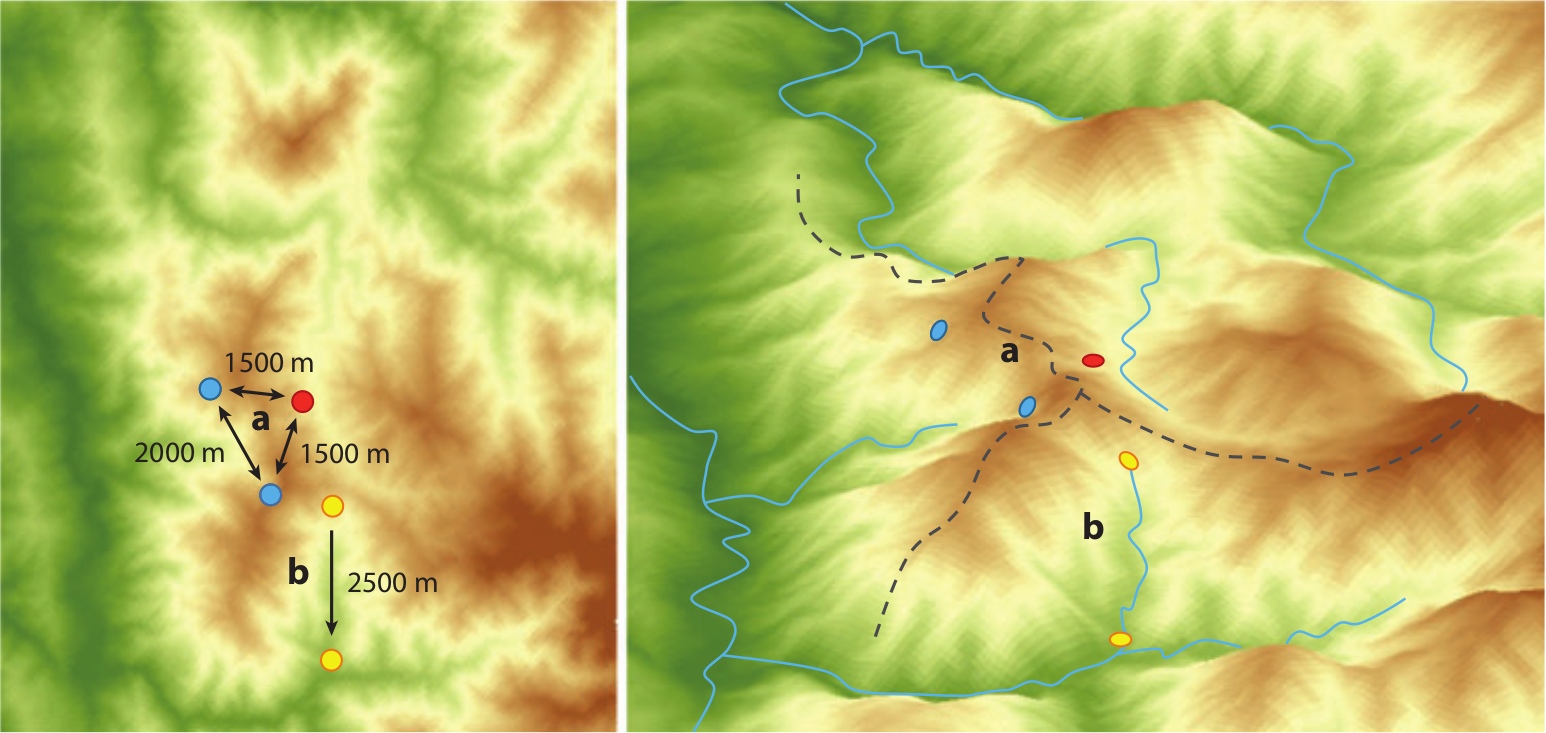
\includegraphics[width=1\textwidth]{images/paisajes_heterogeneos}%
    \caption{La propagación y persistencia a través de paisajes heterogéneos.}\label{fig:paisajes_h}
    \end{figure}

% con un así se pega acá
  \par La \textbf{\textit{Epidemiología Panorámica}}\cite{nidality, ostfeld_re_emerging}
  (EP) está estrechamente relacionada a su paralela ecológica, la Ecología
  Panorámica, una ciencia con inicios en los años 1930s que se dedica a estudiar
  las interacciones entre los ambientes y la vegetación.
  Sin embargo, los paisajes son espacial y temporalmente dinámicos.
  En simultáneo con el nacimiento de la ecología panorámica como una ciencia,
  Pavlosky estipula el concepto de \textit{nidalidad}\footnote{Se define como
  el foco de la infección. Además, Pavlosky, establece que los focos de
  enfermedades a microescala están determinados por todo el ecosistema \cite{nidality}.}
  (o focalidad) de las enfermedades, donde los patógenos son asociados
  a paisajes (zonas) específicos. Un foco de infección contiene tres elementos
  críticos \cite{reisen_landscape}:
  \begin{enumerate}
    \item Vectores con capacidad de transmisión de la infección
    \item Vertebrados capaces de funcionar como reservorio de la infección
    \item Huéspedes susceptibles, como humanos o animales domésticos
  \end{enumerate}
  El concepto de \textit{focalidad} mezclado con la ecología panorámica
  llevó al nacimiento de la ciencia contemporánea
  \textbf{\textit{Epidemiología Panorámica}}, en la cual las enfermedades
  pueden ser asociadas a distintas características del paisaje o cómo
  la configuración entre el vector, el huésped y el patógeno se intersecan
  dado un clima permisivo para que ello suceda.

\par Por definición, la \textit{EP} integra conceptos y
  enfoques de la ecología vinculada a las enfermedades, con el análisis a
  macroescala de la ecología del paisaje. La intersección de estas perspectivas
  nos habilita a entender cómo es que la configuración espacial y las
  características de la composición del paisaje afectan a los procesos
  epidemiológicos a lo largo y ancho de las áreas geográficas que se
  extienden más allá de los procesos que operan localmente dentro de una sola comunidad.
  Así, la \textit{EP} es más que simplemente establecer
  sectores en el territorio y examinar diferencias en condiciones locales de
  factores bióticos y abióticos entre distintos lugares. La clave es obtener
  información sobre la distribución geográfica de la enfermedad y comprender
  cómo las interrelaciones de los paisajes influencian las interreacciones entre
  individuos susceptibles e infectados.

\par La EP ha sido aplicada en gran variedad de estudios sobre vectores de
  enfermedades. A nivel global, se pueden encontrar contribuciones en esta área
  \cite{herbreteau, kalluri_surveillance, data_driven_prediction} también con
  algunas experiencias de herramientas operativas \cite{bowman_alarm}.
  A su vez, muchos estudios interdisciplinarios fueron llevados a cabo en
  latinoamérica enfocados en la generación de modelos predictivos de riesgo,
  espaciales y temporales, basados en condiciones ambientales derivadas de
  información satelital \cite{enao_gis_y_sr, fuller_costa_rica, madrin_correlating, arboleda_colombia}.
  Por ejemplo, en México, Dumonteil y Gourbiere \cite{mexico}
  estudiaron la relación entre la distribución de la especie Triatoma Dimidiata
  y factores bioclimáticos, para de esta forma desarrollar un modelo predictivo de
  la abundancia domiciliaria por esta especie y las tasas de infección
  por T. Cruzi. Estas predicciones se usaron para construir el primer mapa de
  riesgo de transmisión en la península de Yucatán hallándose que la abundancia de T.
  dimidiata se asocia de forma positiva (por análisis de regresión de Poisson)
  con los cultivos, pastos, precipitación, humedad relativa y la temperatura
  máxima. En particular, en Argentina existen varias experiencias en esta
  dirección. En \cite{rotela_space_time, estallo_prevention, espinosa_temporal} abordan el problema de la epidemia del Dengue dando
  herramientas operacionales \cite{porcasi_operative}.

\par Por ejemplo, en 2011, Argentina comenzó a desarrollar un proyecto operacional
  (Sistema de Alerta Temprana de Salud, HEWS), útil tanto para las autoridades de
  salud como para los investigadores.
  Básicamente, HEWS es un mapeo de riesgo dinámico del dengue para todas las
  ciudades del país. En este producto, cada ciudad es representada por un punto
  al que se le asigna un valor de riesgo para cada año, basado en tecnología
  geoespacial. El trabajo fue realizado en un contexto interdisciplinario e
  interinstitucional. En este sistema \cite{porcasi_operative}, el riesgo se evalúa en cuatro componentes que son: el
  entomológico, el viral, el componente relacionado con las actividades de
  control y finalmente el ambiental. Mientras que los tres primeros componentes
  se generan con el aporte de información de los agentes de salud que trabajan en cada
  ciudad, el cuarto se evalúa a partir de datos satelitales.
  Específicamente el componente ambiental, en la versión inicial del sistema, se
  evalúa con una probabilidad estacionaria de presencia de vectores (igual para
  todo el tiempo) más un componente relacionado con el número de ciclos virales,
  que son una función de la temperatura, diferente para cada ciudad y
  para cada año. El mapa de probabilidad de presencia de especie (modelo de nicho)
  es claramente una gran simplificación y se puede mejorar en base a datos
  satelitales continuos del medio ambiente. Variables como precipitación y
  temperatura, han demostrado, con una variabilidad local, influenciar el
  desarrollo de mosquitos, su supervivencia y actividad de
  oviposición\footnote{Proceso de implantación o difusión de huevos plenamente
  desarrollados a partir del cuerpo de la hembra.} y por ende la abundancia de vectores.

\par Otro ejemplo a destacar en la utilización de éstas técnicas en Argentina es
  el trabajo de German y colaboradores \cite{german_temporal}, en 2017.
  En él desarrollan una metodología completa
  para generar modelos de manera automática y basada en información de libre
  acceso. En particular German \cite{german_temporal} utiliza productos del sensor (MODIS) a bordo
  del satélite Terra y Aqua, pues es uno de los más adecuados para esta
  aplicación particular, debido a su resolución temporal, espectral y espacial.
  MODIS proporciona un conjunto de productos pre-procesados y de libre acceso \cite{terra_aqua_modis}.
  Específicamente, los productos de vegetación (índice de vegetación de diferencia
  normalizada) y temperatura (temperatura de la superficie terrestre) derivados
  de MODIS son ejemplos de variables de percepción remota utilizadas
  en aplicaciones de epidemiologia \cite{porcasi_operative, butt_use_modis}
  incorporadas en \cite{german_temporal}. Otra variable
  ambiental obtenida de satélite que es relevante e incorporada, es el
  \textit{Índice de Agua de Diferencia Normalizada} (NDWI) que evalúa de alguna
  forma el contenido de agua de la cubierta terrestre. Adicionalmente el trabajo de German
  incorpora una estimación de la precipitación desde el espacio a partir de las
  misiones (TRMM) y (GPM) \cite{trmm_mision}.
  Utilizando los datos mencionados como variables independientes,
  desarrollaron modelos temporales de pronóstico de oviposición de \textit{Aedes Aegypti}
  usando un método lineal multivariado. En su trabajo, mencionan que
  realizaron muchos métodos con distintos períodos de tiempo y se llegó a
  construir uno con una buena capacidad de
  predicción ($R^{2} = 0.7 $ utilizando 11 variables ambientales independientes en total)


  \section{Aprendizaje automático}

    \par Existen numerosos autores que han definido el concepto de que una máquina
      aprende. En este trabajo hemos extraído una en particular:
      \begin{framed}
        \begin{center}
          \textit{Se dice que un programa de computadora \textbf{aprende} de experiencia
          $E$ con respecto a alguna tarea $T$ y una métrica de rendimiento $M$, si
          con la experiencia $E$ se incrementa su rendimiento en la tarea $T$,
          medida por $M$.}\\
        \end{center}
        \centering \textbf{Tom Mitchell, 1997} \cite{mitchell_learn}
      \end{framed}

      También, en el mismo libro, Mitchell enuncia que el campo del aprendizaje
      automático se refiere a la cuestión de cómo construir programas
      que mejoren automáticamente con experiencia.
      En ese marco, luego de muchos avances en el área, podemos decir que el
      \textit{Aprendizaje Automático} (ML, por sus siglas en inglés) es un
      enfoque empírico efectivo para regresiones y/o clasificaciones de sistemas
      lineales y no lineales, que pueden involucrar desde unos pocos hasta varios
      cientos de variables.

    \par Además, los métodos de ML se pueden clasificar en
      \textit{supervisados}\cite{supervised_learning} y
      \textit{no-supervisados}\cite{unsupervised_learning}, aunque hoy en día
      existen matices entre estas dos clases\cite{semi_supervised}.
      Los algoritmos que aprenden a través de métodos supervisados son aquellos que
      aprenden una función que mapea un valor de entrada a uno de salida basado
      en pares de ejemplos entrada-salida.
      Los algoritmos que utilizan métodos no-supervisados aprenden
      realizando inferencia de la función que describe la estructura de los datos
      de ejemplo. En este caso, los datos de entrenamiento del algoritmo no son
      etiquetados (no existen pares entrada-salida de ejemplo).

    \par Los algoritmos bajo el enfoque de ML requieren entrenamiento utilizando un
      conjunto de datos que sea representativo del conjunto del problema.
      Además, para lograr modelos que puedan generalizar a datos nunca antes vistos,
      los algoritmos supervisados necesitan, al menos, dos subconjuntos necesariamente
      disjuntos de datos: el conjunto de entrenamiento y el de evaluación\cite{test_val}.


    \par El ML es ideal para aquellos problemas en donde el conocimiento teórico del mismo
      es incompleto o insuficiente, pero se cuenta con un gran conjunto de observaciones.
      Este enfoque se utiliza, de manera creciente a medida que pasa el tiempo y
      el poder de cómputo se incrementa, en gran cantidad de aplicaciones tanto para
      problemas más relacionados al ámbito científico, como para problemas
      industriales. Algunos ejemplos de lo primero van desde problemas de
      procesamiento de lenguaje
      natural\cite{twitt_nlp, cardellino, svm_semantic}, procesamiento de
      imágenes\cite{face_detection, corner_detection, handwritting} hasta aplicaciones
      en el área de la salud\cite{nutrition_prediction, bigdata_health, age_estimation, children}
      y las Geociencias\cite{solar_irradiation, ml_grs, modeling_mineral}.

    \par Estas técnicas han mostrado ser de utilidad para un gran número de
      aplicaciones en Geociencias relacionadas a la tierra, oceanos y atmósfera,
      y en algoritmos de extracción de información bio-geofísica.
      Algunos de los algoritmos de ML más usados en aplicaciones relativas a
      Geociencias y Sensado Remoto (GRS) son las Redes Neuronales Artificiales (ANN),
      Support Vector Machines (SVM), Mapas Auto-organizados (SOM), Árboles de Decisión (DT),
      Random Forests y Algoritmos Genéticos.
      Su aplicación en problemas de GRS es
      relativamente nuevo y extremádamente prometedor. En particular, ANNs son
      usadas para clasificación y la aplicación en pronósticos
      relativos a series de tiempo.

    \par Una exploración en la base bibliográfica \textit{Scopus} (\url{www.scopus.com})
      devuelve más de 2.000 publicaciones que incluyen \textit{remote sensing} y
      \textit{machine learning} donde unas 900 fueron publicadas hasta el 2015, y
      alrededor de 1.200 desde ese año hasta la actualidad. Del total, el 24.5\% se
      corresponde con el área de \textit{Computer Science}, un 21.3\% a
      \textit{Earth and Planetary Sciences}, 16.5\% a \textit{Engineering} y el
      restante 37.7\% se distribuye entre numerosas áreas. Esta búsqueda reflejó
      que China, Estados Unidos, Alemania e Italia son los países con mayor
      producción en este sentido.

    \par A su vez, para tener una noción más exhaustiva sobre los esfuerzos académicos
      al respecto de los tópicos que se tratan en este trabajo, se realizó un búsqueda
      sobre la relación entre algunas de la herramientas que se han utilizado y
      el \textit{remote sensing}.

    \par Se encontró que si se cambian las palabras clave por
      \textit{remote sensing} y \textit{neural network} \textit{Scopus} muestra
      que existen 4.000 publicaciones con esos tópicos, de las cuales alrededor de
      1.500 fueron desde el 2015 hasta la actualidad. Del total, un 23.8\% se
      corresponde con el área de \textit{Computer Science}, un 22.7\% a
      \textit{Earth and Planetary Sciences}, 17.5\% a \textit{Engineering} y el
      restante 36\% se distribuye entre otras áreas; con China,
      Estados Unidos, Italia e India como los paises con mayor producción
      científica en dichas áreas.
      El hecho de que esta búsqueda haya arrojado más resultados que la mencionada
      anteriormente, indica que es posible que los investigadores que estén trabajando
      sobre problemáticas de este tipo, quizás, no están explotando las grandes
      capacidades del área de aprendizaje automático en su extensión y, en vez de
      eso, se están centrando en utilizar ANNs por su alta popularidad.

    \par Otra exploración, esta vez sobre \textit{remote sensing} y \textit{k nearest},
      arroja unos 1.100 resultados, de los cuales 310 fueron publicados desde
      el año 2015 a la actualidad. Esta vez, del total de publicaciones encontradas,
      un 25.7\% se corresponde con \textit{Earth and Planetary Sciences}, 16.1\%
      a \textit{Computer Science} y 15\% a \textit{Engineering}. Para este caso,
      Estados Unidos lidera fuertemente la lista de paises con más producción,
      con 387 trabajos. China y Alemania lo siguen con 320 publicaciones entre
      los dos.


    \par A continuación, expondremos de manera más detallada
      herramientas y métodos que motivaron el desarrollo del presente
      trabajo. Enfocaremos en los métodos de regresión, dado que es ésta la clase
      de problema que abordaremos. A su vez, los algoritmos que describiremos son
      los implementados por la librería \textit{Scikit-learn}\cite{scikit-learn}.


  \subsection{Métodos Lineales}

    \par En este trabajo utilizamos dos tipos de regresiones lineales. La regresión
    lineal ordinaria, correspondiente al método de \textit{Mínimos Cuadrados}\cite{least_square}
    y método de regresión \textit{Ridge}\cite{ridge}.
    Dada su popularidad y simplicidad, no ahondaremos en explicaciones profundas
    con el fin de evitar detalles tediosos, muy conocidos.


  \subsection{Árboles de Decisión}
    \par Los \textit{Árboles de Decisión} (DTs, por sus siglas en inglés)\cite{decision_tree_regression}
      son métodos no paramétricos de aprendizaje supervisado
      utilizados tanto para problemas de clasificación como de regresión.
      La meta es crear un modelo que prediga el valor de una variable objetivo aprendiendo
      simples reglas de decisión inferidas a partir de las características de los datos
      de entrenamiento.


    \par El algoritmo de aprendizaje de los DT construye modelos de clasificación o regresión
      utilizando una estructura arbórea. Éste divide el conjunto de datos en pequeños
      subconjuntos mientras que, al mismo tiempo, un árbol de decisión es incrementalmente
      construido. El resultado final es un árbol con nodos de decisión y nodos hojas.
      Un nodo de decisión tiene dos o más ramas, cada una representando valores para
      el atributo examinado. Un nodo hoja representa una decisión dentro del
      objetivo numérico. Los árboles de decisión pueden manejar tanto datos
      categóricos como numéricos.


    \par Más formalmente, dados vectores de entrenamiento $x_{i} \in \mathbb{R}^{n}$, $i = 1,..,l$
      y un vector de etiquetas $y \in \mathbb{R}^{l}$, un árbol de decisión particiona
      recursivamente el espacio de modo que las muestras con la misma etiqueta se agrupen juntas.


    \par Supongamos que los datos en el nodo $m$ son representados por el conjunto $Q$. Para cada
      candidato se divide $\theta = (j, t_{m})$ donde $j$ es una característica y
      $t_{m}$ es un umbral, particionando los datos en conjuntos $Q_{izq}(\theta)$ y
      $Q_{der}(\theta)$ donde:
      \begin{align}
        Q_{izq}(\theta) &= (x, y) | x_{j} \leq t_m \\
        Q_{der}(\theta) &= Q - Q_{izq}(\theta)
      \end{align}


      La impureza en $m$ es calculada usando la función de impureza $H$. La elección
      de ésta depende de la tarea que se quiera realizar.
      En el caso de una regresión, los criterios
      para minimizar en cuanto a la determinación de ubicaciones para las divisiones
      suelen ser el \textbf{Error Cuadrático Medio}, que minimiza el error $L2$\cite{l2_l1_reg} usando
      valores promedios en los nodos terminales, y el \textbf{Error Absoluto Medio}, que minimiza
      el error $L1$\cite{l2_l1_reg} usando el valor de la mediana estadística en los nodos terminales.
      Y así, una vez seleccionada la función de impureza, para el nodo $m$, representando una región $R_{m}$ con una cantidad $N_{m}$ observaciones
      se define la función $G$ de la siguiente manera:
      \begin{align}
        G(Q, \theta) = \frac{n_{izq}}{N_{m}} \ H(Q_{izq}(\theta)) + \frac{n_{der}}{N_{m}} \ H(Q_{der}(\theta))
      \end{align}
      y se seleccionan los parámetros que minimicen la impureza tal como expresa la
      siguiente ecuación
      \begin{align}
        \theta^{*} = argmin_{\theta} \ G(Q, \theta)
      \end{align}

      Luego se sigue partiendo $Q_{izq}$ y $Q_{der}$ hasta que se alcance la profundidad
      máxima permitida del árbol, $N_{m} < min_{muestras}$ o bien $N_{m} = 1$.


  \subsection[Random Forest]{Random Forest\footnote{Dentro de la comunidad técnica, algunos
  algoritmos se referencian utilizando los términos en inglés
  aunque el idioma en el cual se expresen sea el castellano.}}

    \par \textit{Random Forest} (RF) es un método de aprendizaje que utiliza ensamblado de DTs y se
      usa para llevar a cabo tareas tanto de clasificación como de regresión.
      La idea es construir una variedad de árboles de decisión en tiempo de entrenamiento
      y devolver la clase que se corresponda con la moda estadística de las clases
      (para clasificación) o bien el promedio (para regresión) de los resultados
      obtenidos por los árboles individuales.

    \par Existen varios algoritmos de RF. Describiremos formalmente el desarrollado
      por Breiman \cite{random_forest}.
      Sea $\mathcal{D}_{n} = \ \{ (X_{1}, Y_{1}), \ \dots, \ (X_{n}, Y_{n})\}$
      un conjunto de variables aleatorias independientes e idénticamente distribuídas (i.i.d.)
      pertenecientes al conjunto $[0,1]^{d} \ \times \ \mathbb{R} $ con $d \geq 2$,
      con la misma distribución que un par genérico $(X,Y)$ satisfaciendo que
      $\mathbbm{E}Y^{2} < \infty$. Además, sea $r()$ la función de regresión que se busca estimar.

    \par Un RF es un predictor que consiste de una colección aleatoria base
      de árboles de regresión, $\{ r_{n}(x, \theta_{m}, \mathcal{D}_{n}), m \ > \ 1 \}$, donde
      $\theta_{1},\ \theta_{2},\ \dots$ son salidas i.i.d. de una variable aleatoria
      $\theta$. Éstos árboles aleatorios son combinados para formar la estimación
      de la regresión:

      \begin{align}
        \overline{r}(X,\ \mathcal{D}_{n})\ =\ \mathbbm{E}_{\theta}[r_{n}(X,\ \theta,\ \mathcal{D}_{n})]
      \end{align}

      donde $\mathbbm{E}_{\theta}$ denota la esperanza con respecto al parámetro aleatorio
      condicionada por $X$ y el conjunto de datos $\mathcal{D}_{n}$. Notemos que
      dicha esperanza es evualuada por el método de Monte Carlo\cite{monte_carlo},
      esto es, generando $M$ árboles aleatorios, y tomando el promedio de los resultados.
      La variable de aleatoriedad $\theta$ es usada para determinar cómo se van a realizar los
      sucesivos cortes cuando se construyen los árboles individuales, como una selección
      de la coordenada a dividir y la posición de la división.

    \par Cada árbol aleatorio es construido de la siguiente manera: todos los nodos
      del árbol son asociados a celdas rectangulares tales que en cada etapa de
      construcción del árbol, el conjunto de celdas asociadas a las hojas del árbol
      forman una partición de $[0, 1]^{d}$. La raíz del árbol es exactamente $[0, 1]^{d}$.
      Luego, el siguiente procedimiento es repetido una cantidad $\lceil \log_{2}k_{n} \rceil$ veces
      donde $k_{n}$ es un parámetro determinístico, fijado por el usuario, posiblemente
      dependiente del valor de $n$.

      \begin{enumerate}
        \item En cada nodo, se selecciona una coordenada de $X = (X^{(1)}, \ \dots,\ X^{(d)})$
              donde la característica j-ésima tiene una probabilidad de $p_{nj} \in (0,1)$
              de ser elegida.
        \item En cada nodo, una vez que la coordenada es seleccionada, la división es
              en el punto intermedio del lado elegido.
      \end{enumerate}

      Cada árbol aleatorio $r_{n}(X, \theta)$ devuelve el promedio sobre todos los
      $Y_{i}$ para los cuales los vectores correspondientes $X_{i}$ caen en la misma
      celda de la partición aleatoria que $X$.


  \subsection{K-Vecinos más cercanos (KNN)}
    \par El principio detrás de los métodos de vecinos más cercanos es encontrar un
      número predefinido de las muestras de entrenamiento más cercanas en distancia
      al nuevo punto, y predecir su valor a partir de ellos.
      El número de muestras puede ser una constante definida por el usuario, o
      variar basada en la densidad local de los puntos. La distancia puede, en general,
      ser cualquier métrica aunque la distancia Euclídea es la elección más común.

    \par Las predicciones son hechas para un nuevo punto $x$, buscando a través del conjunto
      de entrenamiento completo las $K$ instancias más cercanas (los vecinos) y computar
      la variable de retorno utilizando la información de esos K puntos. Para el caso
      de la regresión suele ser el promedio de cada variable de retorno de la siguiente
      manera

      \begin{align}
        \overline{y}(x) = \frac{1}{k} * \sum_{j \in knn(x)} y_{j}
      \end{align}



  \subsection{Support Vector Machine (SVM) y \textit{Support Vector Regression} (SVR)}

    \par Una \textit{Support Vector Machine} (SVM) \cite{first_svm} construye un
      hiperplano o un conjunto de hiperplanos en un espacio
      de muy alta, o infinta, dimensionalidad. Éstos pueden ser usados tanto para
      tareas de regresión como de clasificación. Intuitivamente, una buena separación
      se consigue por el hiperplano que tenga la mayor distancia a los puntos de
      entrenamiento más cercanos de alguna clase, como se puede observar en la
      Figura \ref{fig:svm}, dado que en general
      a más grande sea esa distancia más pequeño será el error de generalización del
      modelo.

    \par \textit{Support Vector Regression} (SVR)\cite{support_vector_regression, review_svr}
      es una veloz y precisa forma de interpolación de conjuntos de datos.
      Es útil cuando se quiere aproximar una función costosa de calcular sobre un
      dominio conocido. Aprende rápidamente y se puede mejorar sistemáticamente.

      \begin{figure}
      \centering%
      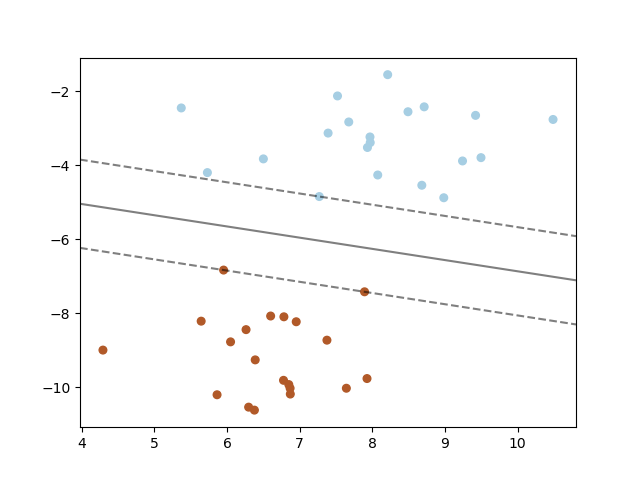
\includegraphics[width=0.5\textwidth]{images/svm_hiperplane}%
      \caption{Plano de separación de clases generado por una SVM.}\label{fig:svm}
      \end{figure}

    \par SVR es una generalización de la SVM a problemas de regresión. Técnicamente,
      se puede decir que es un algoritmo de aprendizaje supervisado. Éste
      requiere de un conjunto de datos de entrenamiento,
      $\mathcal{T} = (\vec{X}, \vec{Y})$, que cubre el dominio de interés acompañado
      de las soluciones en dicho dominio. El trabajo de la SVM es aproximar la función
      definida por el conjnuto de entrenamiento, $F(\vec{X}) = \vec{Y}$. En general,
      en las SVM, los vectores $\vec{X}$ son utilizados para definir el hiperplano que
      separa las distintas soluciones posibles. En problemas de regresión, estos
      vectores son utilizados para realizar una regresión lineal. Los que estén
      más cerca del punto de prueba se los llama \textit{vectores de soporte}.

      Daremos una idea más detallada de los fundamentos matemáticos detrás de una
      SVR \cite{svr_tutorial}:
      Dados los vectores de entrenamiento $x_{i} \in \mathbb{R}^{p}$ con $i = 1, \dots ,n$
      y un vector $y \in \mathbb{R}^{n}$, el $\epsilon$-SVR resuelve el siguiente problema
      primario:
      \pagebreak
        \begin{align}
          \min\limits_{w, b, \zeta, \zeta^{*}} \frac{1}{2} w^{T} w + C \sum_{i = 1}^{n} \zeta_{i}
        \end{align}
      con las restricciones de:

      \begin{math}
        y_{i} - w^{T} \phi(x_{i}) - b \leq \epsilon + \zeta_{i}, \\
        w^{T} \phi(x_{i}) + b - y_{i} \leq \epsilon + \zeta^{*}_{i}, \\
              \zeta^{*}_{i}, \zeta_{i} \geq 0 \\
        para\ i\ =\ 1,\ \dots, n
      \end{math}

      Mientras que el problema dual a resolver es:

      \begin{align}
        \min\limits{\alpha, \alpha^{*}} \frac{1}{2} (\alpha - \alpha^{*})^{T}
        Q(\alpha - \alpha^{*}) + \epsilon e^{T} (\alpha + \alpha^{*}) -
        y^{T} (\alpha - \alpha^{*})
      \end{align}
      con las restricciones de:

      \begin{math}
        e^{T} (\alpha - \alpha^{*}) = 0, \\
        0 \geq \alpha, \alpha^{*} \leq C \\
        para\ i\ =\ 1, \dots, n
      \end{math}
    . Donde $e$ es un vector para el cual todos sus componentes poseen el valor $1$, $C > 0$
      es la cota superior, $Q$ es una matriz semidefinida
      positiva\footnote{Una matriz, $M$, es semidefinida positiva si $x^{*}Mx \leq 0$
      $\forall x \in \mathbb{R}^{n}$.} de tamaño $n \times n$,
      $Q_{ij} \equiv K(x_{i}, x_{j}) = \phi(x_{i}^{T})\phi(x_{j})$ es el núcleo
      (\textit{kernel}, en inglés). Aquí, los vectores de entrenamiento están siendo mapeados
      a un espacio de gran (probablemente infinita) dimensionalidad por la función
      $\phi$.
      Luego, la función de decisión es:
      \begin{align}
        \sum_{i = 1}^{n} (\alpha - \alpha^{*})K(x_{i}, x) + \rho
      \end{align}

  \subsection{Perceptron Multicapa (MLP)}

    \par Un \textbf{Perceptron Multicapa} (MLP, por sus siglas en inglés)\cite{mlp_intro1, mlp_intro2} es un tipo
      de red neuronal artificial (ANN) \textit{feedforward}.
      Es un algoritmo de aprendizaje supervisado que logra distinguir
      relaciones entre datos que no sean linealmente separables. Aprende una función
      a partir de un conjunto de datos de entrenamiento y puede ser
      utilizada tanto para tareas de regresión como de clasificación haciendo uso, entre
      otras cosas, de una técnica llamada \textit{propagación hacia atrás}\cite{backpropagation}
      (\textit{backpropagation}, en inglés).
      El MLP consiste de al menos tres capas: una de entrada, una de salida y,
      como mínimo, una capa oculta\footnote{Una capa de neuronas artificiales que toman un conjunto
      de entradas ponderadas y producen una salida a través de una función de activación.};
      la vista gráfica de una arquitectura simple se puede observar en la
      Figura \ref{fig:mlp_ejemplo}.
      \begin{figure}
      \centering%
      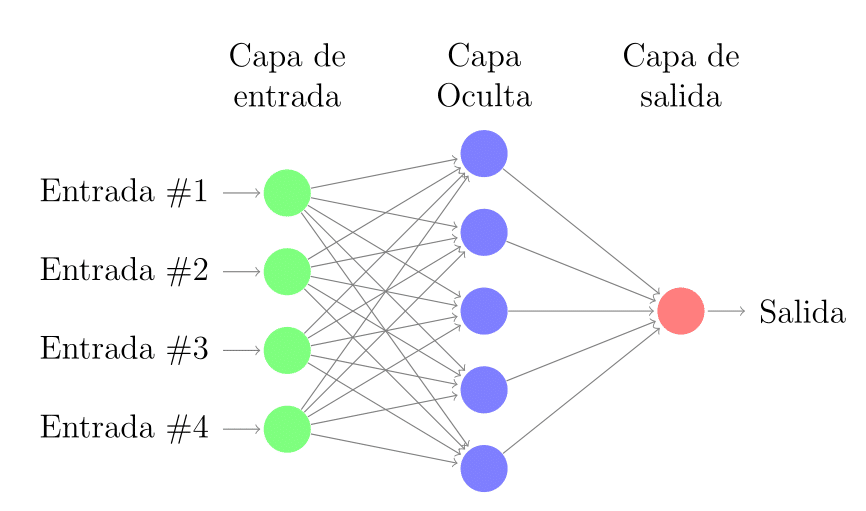
\includegraphics[width=0.7\textwidth]{images/ejemplo_mlp}%
      \caption{Arquitectura de una MLP de cuatro variables de entrada, una capa
              oculta de cinco neuronas y un sólo valor de salida.}\label{fig:mlp_ejemplo}
      \end{figure}

    \par Una descripción matemática simplificada del algoritmo en cuestión es la
      que se menciona a continuación.
      Dados ejemplos de entrenamiento $(x_{1}, y_{1}), \dots, (x_{n}, y_{n})$
      donde $x_{i} \in \mathbb{R}^{m}$ y $y_{i} \in \{0,1\}$, un MLP de una capa oculta
      con una neurona aprende una función $f(x) = W_{2}g(W_{1}^{T} x + b_{1}) + b_{2}$
      donde $W_{1} \in \mathbb{R}^{m}$ y $W_{2}, b_{1}, b_{2} \in \mathbb{R}$ son
      parámetros del modelo. $W_{1}, W_{2}$ representan los pesos de la capa de entrada y la
      capa oculta, respectivamente. $b_{1}, b_{2}$ representan el sesgo agregado a
      la capa oculta y la capa de salida, respectivamente. La función
      $g: \mathbb{R} \rightarrow \mathbb{R}$ es la función de activación, la cual
      es definida por defecto como la tangente hiperbólica. Está dada por,

      \begin{align}
        g(z) = \frac{e^{z} - e^{-z}}{e^{z} + e^{-z}}
      \end{align}

      En problemas de regresión, la salida del algoritmo es $f(x)$, por lo que la
      función de activación de salida es simplemente la función identidad. En estos
      problemas, MLP también utiliza como función de pérdida la correspondiente
      al \textit{Error Cuadrático}:
      \begin{align}
        Loss(\hat{y}, y, W) = \frac{1}{2} \norm{\hat{y} - y}^{2}_{2} + \frac{\alpha}{2} \norm{W}^{2}_{2}
      \end{align}



    \par Comenzando desde pesos con valores aleatorios, el MLP minimiza la función de
      pérdida actualizando repetidamente dichos pesos. Luego de calcular la pérdida,
      se propaga desde la capa de salida a todas las anteriores (\textit{backpropagation}),
      proporcionando un valor de peso a cada parámetros para disminuir la pérdida.
      Para ello, se utiliza \textit{descenso por gradiente}, en el cual el
      gradiente $\nabla Loss_{W}$ de la pérdida con respecto a los pesos es
      calculada y deducida de W.
      Más formalmente, es expresado como:
      \begin{align}
        W^{i + 1} = W^{i} - \epsilon \nabla Loss^{i}_{W}
      \end{align}
      donde $i$ es el paso de iteración, y $\epsilon > 0$ es la taza de aprendizaje.

      En general el algoritmo termina cuando se alcanza cierto número definido por el
      usuario de iteraciones o se cruza un umbral para la pérdida.


%\end{document}

\documentclass[12pt,spanish,fleqn,openany,letterpaper,pagesize]{scrbook}

\usepackage[utf8]{inputenc}
\usepackage[spanish]{babel}
\usepackage{fancyhdr}
\usepackage{epsfig}
\usepackage{epic}
\usepackage{eepic}
\usepackage{amsmath}
\usepackage{threeparttable}
\usepackage{amscd}
\usepackage{here}
\usepackage{graphicx}
\usepackage{lscape}
\usepackage{tabularx}
\usepackage{subfigure}
\usepackage{longtable}


\usepackage{rotating} %Para rotar texto, objetos y tablas seite. No se ve en DVI solo en PS. Seite 328 Hundebuch
                        %se usa junto con \rotate, \sidewidestable ....


\renewcommand{\theequation}{\thechapter-\arabic{equation}}
\renewcommand{\thefigure}{\textbf{\thechapter-\arabic{figure}}}
\renewcommand{\thetable}{\textbf{\thechapter-\arabic{table}}}


\pagestyle{fancyplain}%\addtolength{\headwidth}{\marginparwidth}
\textheight22.5cm \topmargin0cm \textwidth16.5cm
\oddsidemargin0.5cm \evensidemargin-0.5cm%
\renewcommand{\chaptermark}[1]{\markboth{\thechapter\; #1}{}}
\renewcommand{\sectionmark}[1]{\markright{\thesection\; #1}}
\lhead[\fancyplain{}{\thepage}]{\fancyplain{}{\rightmark}}
\rhead[\fancyplain{}{\leftmark}]{\fancyplain{}{\thepage}}
\fancyfoot{}
\thispagestyle{fancy}%


\addtolength{\headwidth}{0cm}
\unitlength1mm %Define la unidad LE para Figuras
\mathindent0cm %Define la distancia de las formulas al texto,  fleqn las descentra
\marginparwidth0cm
\parindent0cm %Define la distancia de la primera linea de un parrafo a la margen

%Para tablas,  redefine el backschlash en tablas donde se define la posici\'{o}n del texto en las
%casillas (con \centering \raggedright o \raggedleft)
\newcommand{\PreserveBackslash}[1]{\let\temp=\\#1\let\\=\temp}
\let\PBS=\PreserveBackslash

%Espacio entre lineas
\renewcommand{\baselinestretch}{1.1}

%Neuer Befehl f\"{u}r die Tabelle Eigenschaften der Aktivkohlen
\newcommand{\arr}[1]{\raisebox{1.5ex}[0cm][0cm]{#1}}

%Neue Kommandos
\usepackage{Befehle}


%Trennungsliste
\hyphenation {Reaktor-ab-me-ssun-gen Gas-zu-sa-mmen-set-zung
Raum-gesch-win-dig-keit Durch-fluss Stick-stoff-gemisch
Ad-sorp-tions-tem-pe-ra-tur Klein-schmidt
Kohlen-stoff-Mole-kular-siebe Py-rolysat-aus-beu-te
Trans-port-vor-gan-ge}

\begin{document}

\justifying
\chapter{Modelando la Población del Vector de Dengue Utilizando Datos de Sensado Remoto y Aprendizaje Automático}

  \par Como mencionamos en capitulos anteriores, en un trabajo interinstitutional entre
    la Comisión Nacional de Actividades Espaciales (CONAE) y el ministerio de salud
    de Argentina, hubo iniciativas orientadas a modelar la evolución temporal de
    las poblaciones de mosquitos usando variables ambientales obtenidas de
    sensores remotos. Estos trabajos utilizaron series de algunos años y fueron
    basadas en un pequeño número de variables satelitales \cite{ndwi_erffectiveness, modis_data}.
    En un esfuerzo para mejorar esto, \cite{temporal_modeling}, construyeron modelos
    de series temporales de cuatro años, basados en una gran cantidad de variables
    de varios sensores.
    Aún así, todos estos trabajos asumieron modelos lineales multivariados.

  \par El trabajo presentado en este capítulo representa una mejoría sobre
    dicho escenario. Comparamos
    Support Vector Machines (SVM), Redes Neuronales Artificiales (ANN),
    K-vecinos más cercanos (KNN) y un tipo de árbol de decisión orientado a
    regresión, sumados a dos modelos de regresión lineal. Con ésto, se
    obtiene una metodología operacional que contribuye al sistema de riesgo
    de Dengue actualmente en operación \cite{porcasi_operative, analisis_cordoba}.

  \par Se explora, en contraste con los trabajos previos mencionados, la habilidad
    de modelado y predicción de oviposición con algoritmos de Aprendizaje
    Automático \textit{off-the-shelf}, i.e. algoritmos de software libre, ya
    implementados, sin mayores desarrollos sobre lo existente y con un ajuste de
    hiperparámetros minimo. De ésta manera se busca la asimilación de estas
    técnicas a toda la comunidad que se ocupa de problemas similares.


\section{Materiales}

\subsection{Datos de estudio y Datos de Campo}
  \begin{figure}[hbt]
  \centering%
  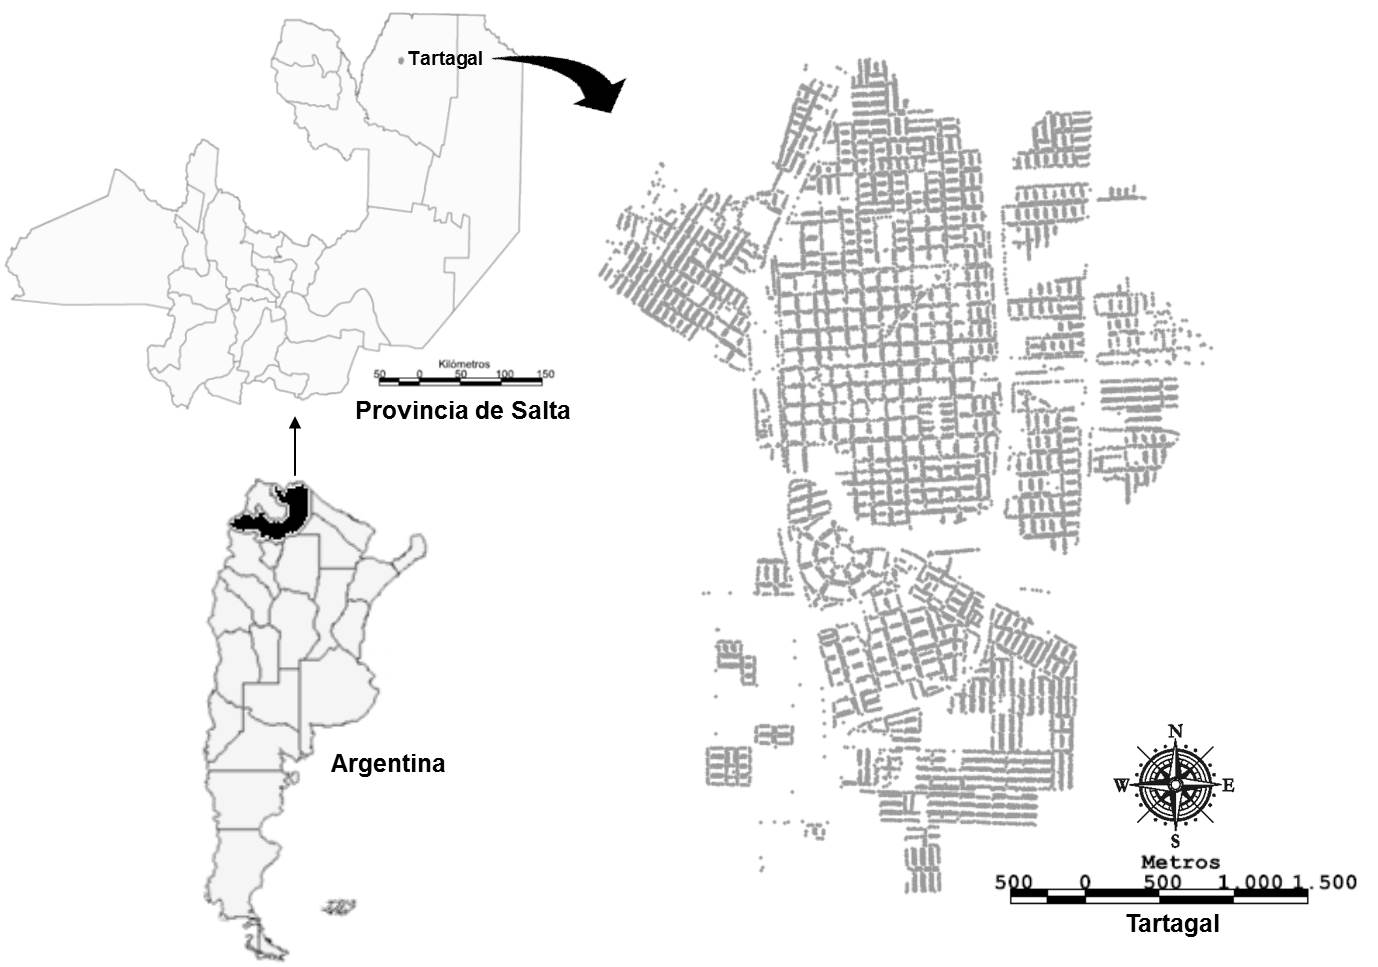
\includegraphics[width=0.6\textwidth]{images/tartagal}%
  \caption{Área de Estudio}\label{fig:tartagal}
  \end{figure}

  \par El estudio presentado fue desarrollado en la ciudad de Tartagal
    (con 79.900 habitantes) en el noroeste de Argentina
    (\ang{22;32;}~S, \ang{63;49;}~O, \SI{450}{\meter} sobre el nivel del mar),
    en la provincia de Salta. El sitio está entre 50 y 100 kms de la frontera
    entre Argentina y Bolivia, como se puede apreciar en la Figura \ref{fig:tartagal}

  \par Este lugar tiene una temperatura media anual de unos \SI{23}{\degreeCelsius}
    (máximo promedio de verano de \SI{39}{\degreeCelsius} y minimo promedio en
    invieron de \SI{9}{\degreeCelsius}). Tiene una precipitación anual de
    \SI{1100}{\milli\meter}, con una estación seca (Junio a Octubre).
    Tartagal, como muchas ciudades del noroeste argentino, tiene una diversidad
    cultural basada en la presencia de grupos étnicos autóctonos y población
    de inmigrantes sumada al movimiento de migración proveniente de Bolivia.
    Estas características conducen a un perfil peculiar de comportamiento
    cultural, social y economico.

  \par La población de vectores es medida monitoreando la actividad de oviposición.
    Es medida usando ovitrampas colocadas en casas aleatoriamente seleccionadas
    en el área urbana de la ciudad. El período de monitoreo utilizado en este
    estudio fue de Agosto de 2012 hasta Julio de 2016 sobre 50 casas. Dos
    ovitrampas fueron colocadas en cada una: una dentro y otra fuera de la casa,
    en el patio trasero en un lugar con sombra y a nivel del suelo, siguiendo
    las instrucciones de la OMS \cite{peridomestic}. Las ovitrampas son contenedores
    de \SI{1000}{\centi\meter\cubed} de plástico negro con \SI{250}{\milli\liter}
    de agua sin ninguna infusión de atracción.
    En este estudio sólo utilizamos los datos de las ovitrampas externas dado
    que ellas tienen una mayor correlación con las variables ambientales
    derivadas de información satelital. Dichas ovitrampas son reempazadas
    semanalmente y los huevos son contados en un laboratorio de acuerdo al
    \textit{Indice de Densidad de Huevos} \cite{indice_huevos}. Luego, la
    actividad de oviposición del \textit{Aedes Aegipty} es estimada por la suma
    de los huevos capturados en las trampas externas de la ciudad.



\subsection{Variables Ambientales}

  \par Siguiendo la idea de construir modelos predictivos de la población de
    vectores basados en variables ambientales derivadas de satelites, pero con una
    perspectiva operacional basada en trabajos previos, se obtuvieron representaciones
    de vegetación, humedad, temperatura y lluvia operacionalmente disponibles
    de \textbf{MODIS} y productos \textbf{TRMM/GPM}.

  \par Los índices de vegetación global proveen productos espaciales y
    temporales consistentes sobre la cobertura verdosa de la vegetación,
    propiedades del área foliar y el nivel de clorofila. Estos indices son
    derivados de la reflectancia atmosférica
    corregida en las bandas infrarroja (MIR) e infrarroja cercana (NIR).
    En este caso se utiliza el \textbf{NDVI} de producto satelital
    de MODIS, \textit{MOD13Q1}, (compuesto de 16 días) con una resolución espacial de
    \SI{250}{\meter}.
    Las condiciones de vegetación son incluidas junto con la temperatura,
    humedad y precipitación, son variables relevantes para la evolución de la
    población de mosquitos \cite{ndwi_erffectiveness, rs_invertebrate}.

  \par A su vez, se incluye el Indice de Agua de Diferencia Normalizada
    (\textbf{NDWI}), que está vinculado al contenido de agua líquida y humedad
    tanto en la vegetación como en estructuras sólidas.
    Es calculada a partir del mismo producto MODIS usando la definición de
    \textit{Gao} \cite{gao_ndwi} del NDWI desde las bandas provistas por
    el producto \textit{MOD13Q1}, correspondiente a la reflectancia de MIR y NIR:
    $NDWI =  (\rho_{NIR} - \rho_{MIR}) / (\rho_{NIR}  + \rho_{MIR} ) \times 10^4$
    Los productos MODIS, en general, necesitan el factor $10^{4}$ para ser guardados,
    por eficiencia computacional, como números enteros.

  \par En este trabajo, adicionalmente, utilizamos la Temperatura De la Superficie
    Terrestre (\textbf{LST}) de MODIS dado que es una aproximación de la
    temperatura ambiental \cite{infectious_diseases, surface_temp, temp_algorithm}.
    Para esto, se eligió el producto satelital \textit{MOD11A2}. Tiene una
    resolución espacial de \SI{1}{\kilo\meter} y un promedio de valores de
    LST de cielo-abierto durante un periodo de 8 días. Éste producto incluye
    LST de la noche y el día para así de alguna manera representar
    temperaturas mínimas y máximas \cite{lst_surface}.

  \par La precipitación local es obtenida de la Misión Tropical de Medida de Lluvia
    (\textbf{TRMM}) \cite{trmm_mision}. Ésta es una misión conjunta entre la
    NASA y la Agencia Aeroespacial de Exploración de Japón lanzada en 1997
    para el estudio de las lluvias y así realizar investigaciones sobre el
    clima. Para detectar la lluvia, el satélite utiliza muchos instrumentos
    incluyendo radar, imagenes de microondas y sensores de rayos. TRMM, a pesar
    de que se quedó sin combustible en 2014, siguió transmitiendo datos hasta
    Junio del 2015.
    Luego de eso, otros productos basados en una nueva misión espacial llamada
    GPM (\url{https://earthdata.nasa.gov/trmm-to-gpm}), fueron publicados para
    asegurar la continuidad de estos trabajos.


  \par Dos áreas de \SI{85}{\hectare} fueron definidas alrededor de la ciudad
    y se calcularon los valores medios para todas las variables derivadas de
    satelite. Siguiendo el enfoque de
    \cite{models_predicting, dynamics_of_dengue, temporal_modeling},
    la primer área se encuentra ubicada dentro de la ciudad
    (Área Urbana) y la segunda abarca la vegetacion nativa que rodea la ciudad
    (Área Rural). Ésta elección fue tomada bajo la hipótesis de que seleccionar
    una zona fuera de la ciudad representaría bien las condiciones ambientales
    (NDWI, NDVI, LST). La misma idea fue utilizada en estudios previos muy
    relacionados. Es probable que estas observaciones y los indices de larvas
    estén estrechamente relacionadas. En ese sentido es que el área rural o
    externe fue seleccionada aleatoriamente de aquellas con vegetación suficientemente
    cercana a la ciudad, representando condiciones ambientales naturales.
    En este caso específico esta región rural es seleccionada en el
    noreste de la ciudad; tiene una altitud similar a la ciudad y mayormente
    bosque nativo. Se puede observar en la Figura \ref{fig:zones}.
    \begin{figure}[hbt]
    \centering%
    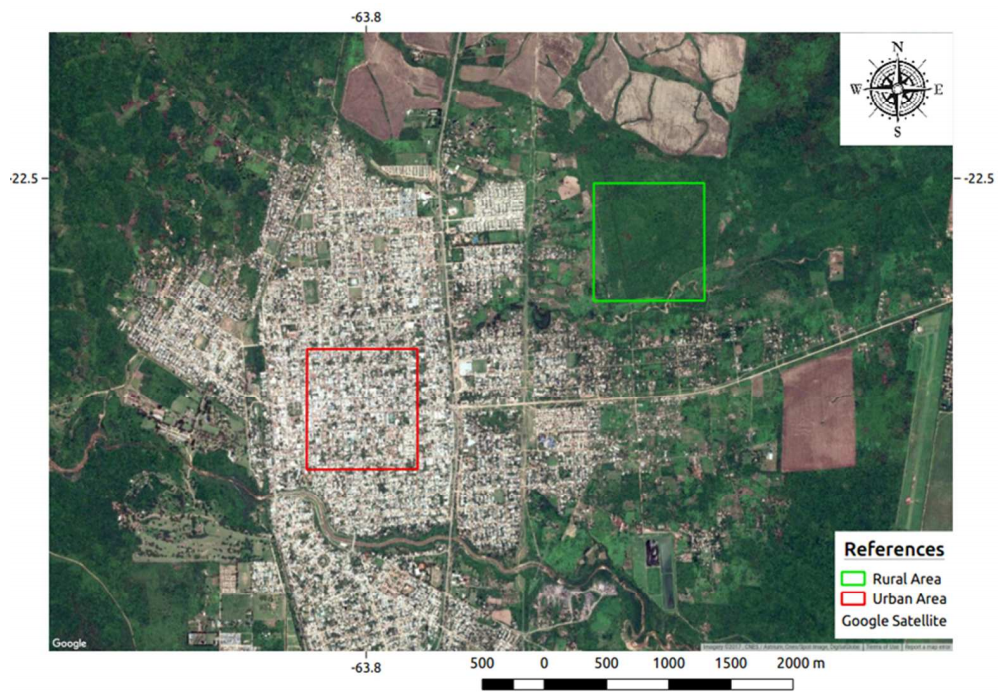
\includegraphics[width=0.6\textwidth]{images/zones}%
    \caption{Areas rural y urbana seleccionadas para extraer las variables ambientales}\label{fig:zones}
    \end{figure}


  \par El procedimiento de construir las series temporales a partir de variables
    provenientes del sensado remoto se describen en la Figura \ref{fig:sistema}.
    Las imagenes son obtenidas de la NASA (\url{http://e4ftl01.cr.usgs.gov}) e
    importadas en \textbf{GRASS 7.1}. Para cada una de las áreas anteriormente
    definidas se calcula la media de cada día. Cada uno de estos valores
    promedio y sos díás son exportadas a una tabla en el software \textbf{R},
    donde es utilizada para construir las series temporales completas.
    Los datos son interpolados para obtener valores para cada uno de los
    días de muestra (un valor para cada semana epidemiológica).
    \begin{figure}[hbt]
    \centering%
    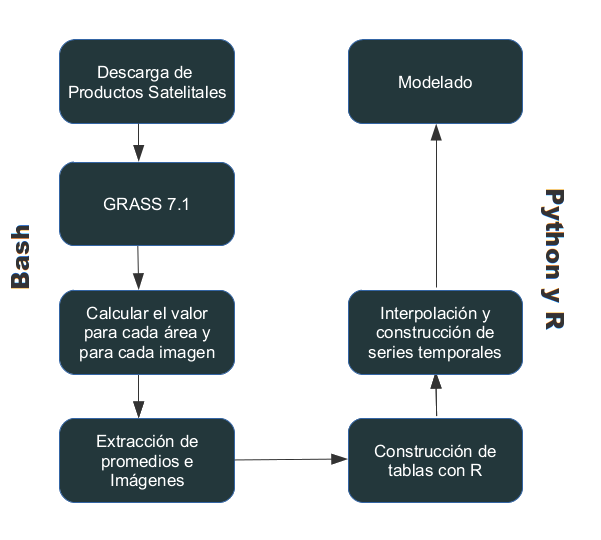
\includegraphics[width=0.6\textwidth]{images/sistema}%
    \caption{Sistema de procesamiento de productos satelitales}\label{fig:sistema}
    \end{figure}

  \par Todas las variables son consideradas con tres semanas de \textit{lag}
    teniendo en cuenta las series temporales originales, para representar las
    influencias asincrónicas, correspondientemente con uno, dos o tres
    lapsos de tiempo.

  \par El primer paso consistió en analizar las cuarenta variables ambientales
    y los huevos recolectados cada semana por medio de una matriz de correlación
    y los valores \textbf{p} que miden su significancia. Ésto llevó a descartar
    treinta y cinco variables. Se prefieren las variables con \textit{lag} dada
    su potencial habilidad de pronóstico. Las siguiente variables fueron
    seleccionadas: NDVI rural \textit{lag} 1, NDWI rural \textit{lag} 1, LST rural dia \textit{lag} 3,
    LST rural noche \textit{lag} 1 y TRMM \textit{lag} 3. Luego, todas las
    variables fueron normalizadas utilizando el \textbf{\textit{z-score}}.

  \par La Figura \ref{fig:heatmap} presenta las variables ambientales junto
    con la oviposición en un mapa de calor (\textit{heatmap}). Este formato
    permite una visualización en la evolución temporal, de los
    patrones de correlación entre las variables y el efecto de \textit{lag}.

    \begin{figure}[hbt]
    \centering%
    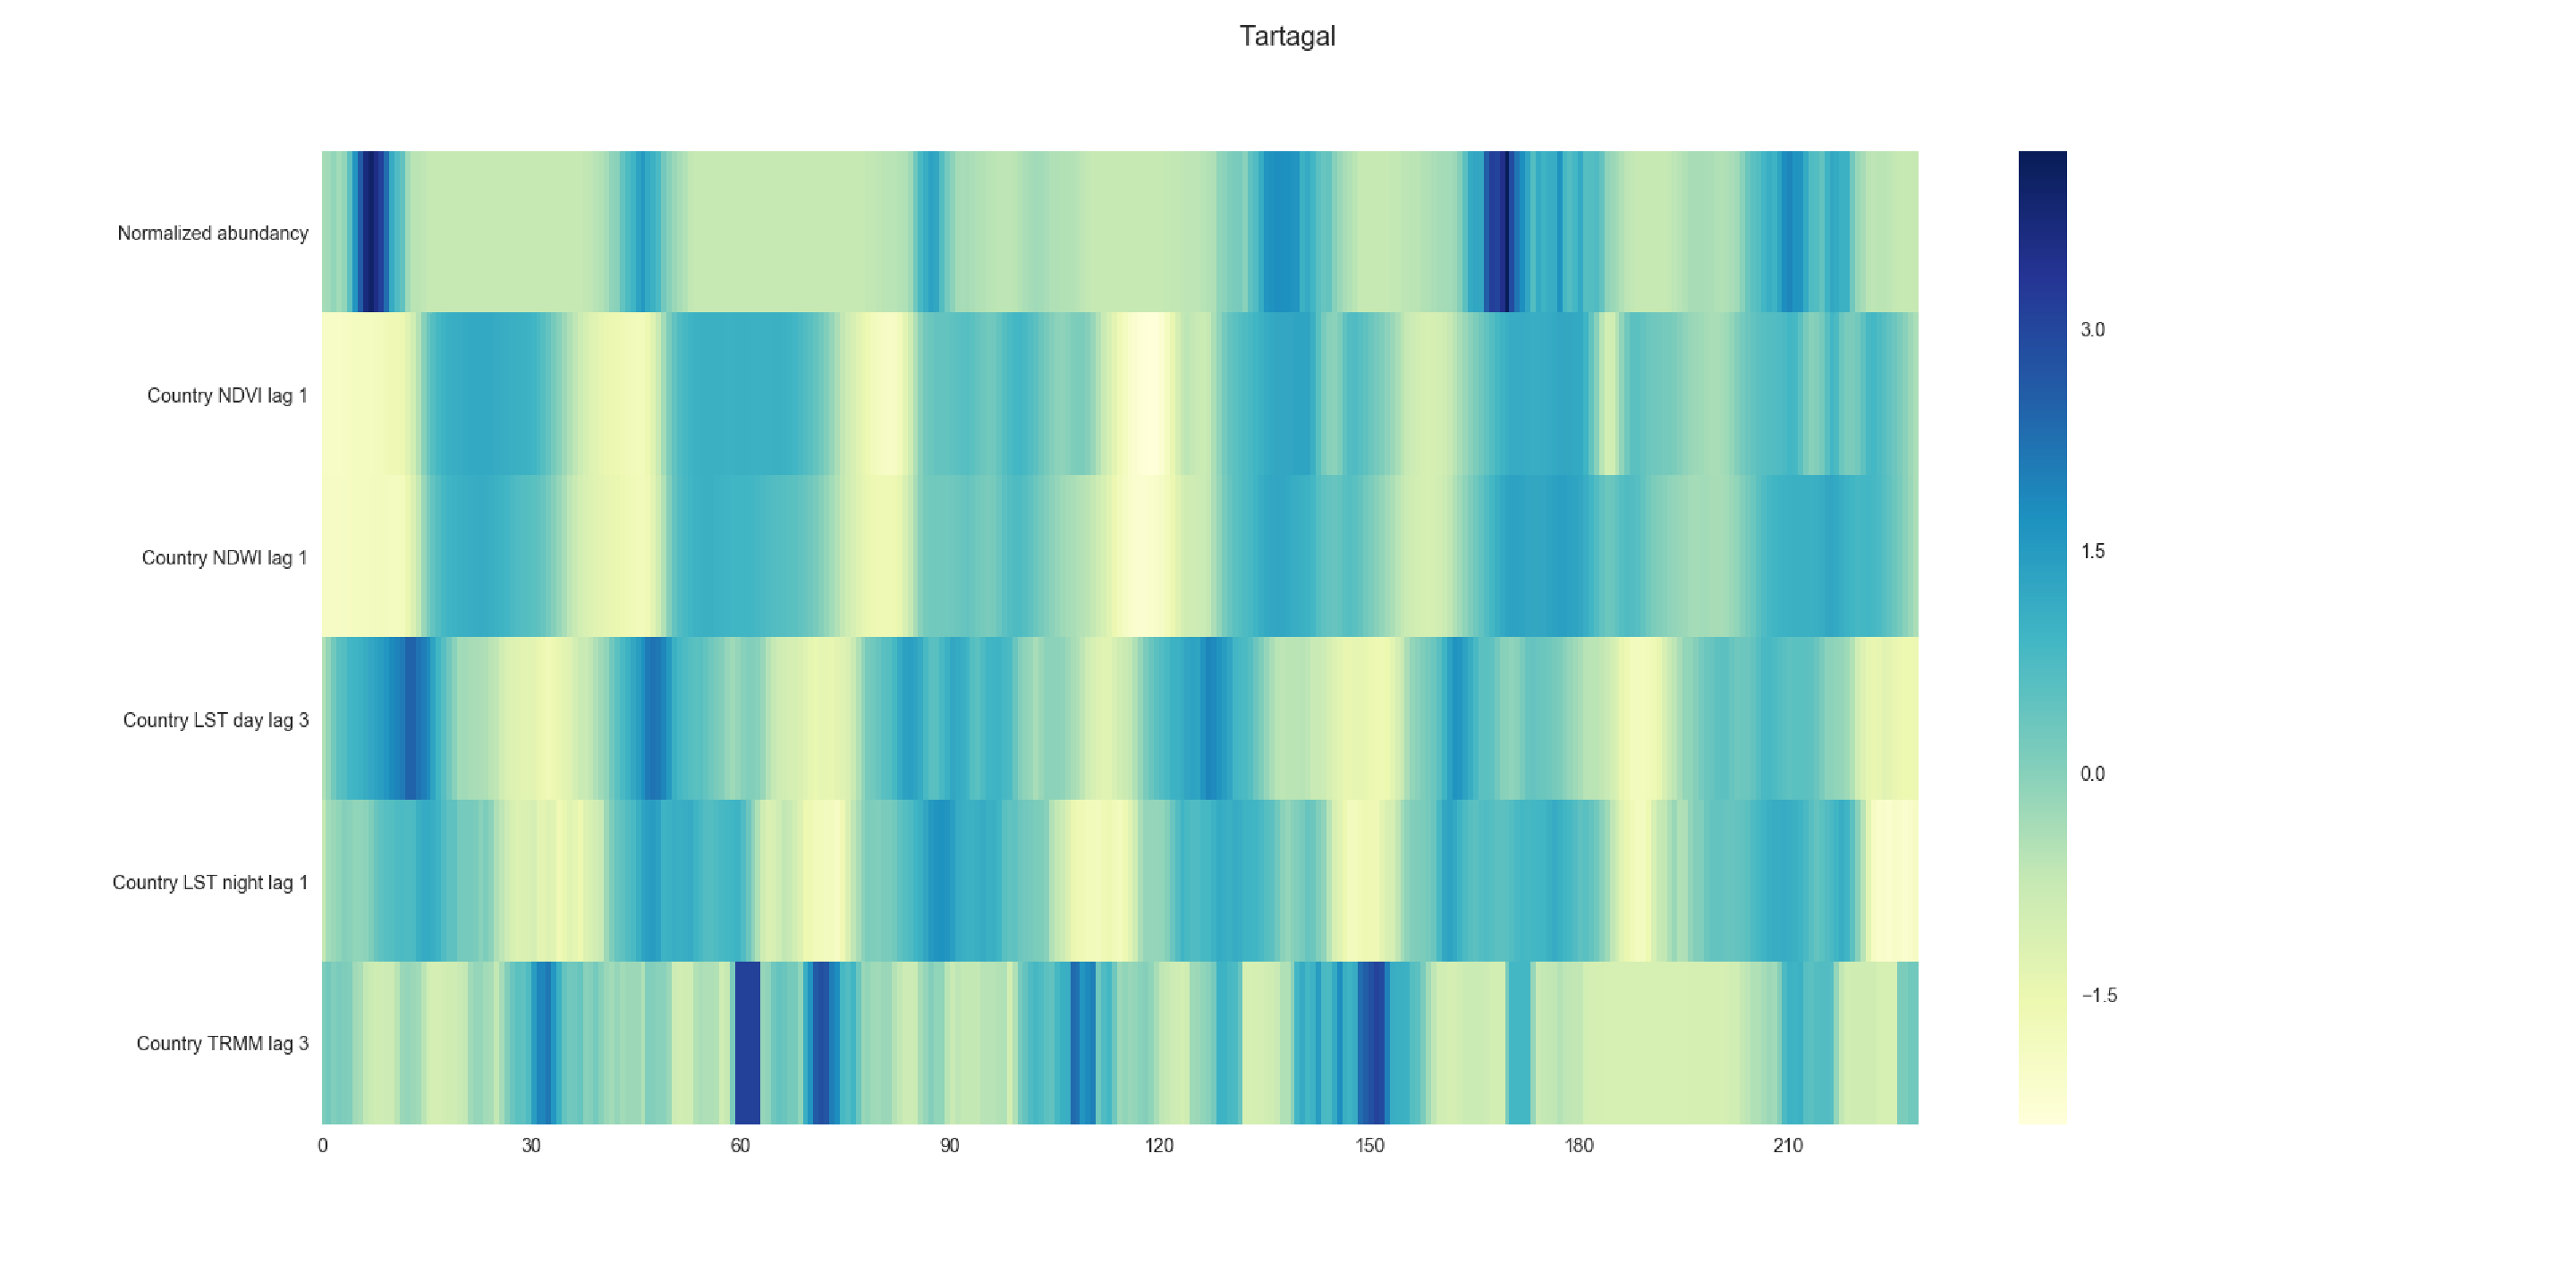
\includegraphics[width=1\textwidth]{images/heatmap}%
    \caption{Heatmap de valores del \textit{z-score} de variables ambientales}\label{fig:heatmap}
    \end{figure}



\section{Modelado}

  \par Con el conjunto de datos descripto en la sección anterior, se implementaron
    dos modelos lineales (tradicional y \textit{Ridge}) y cuatro modelos
    no-lineales (\textit{Support Vector Machine}, ANN Perceptron Multicapa,
    Árbol de Decisión, K-vecinos más cercanos) para modelar la oviposición
    para cada semana. Para todos los modelos se utilizó el mismo conjunto de
    5 variables ambientales como \textit{features}.

  \par En todos los casos se entrenaron los modelos con 80\% del conjunto de
    datos y se utilizó el 20\% restante de la serie temporal (alrededor de un año)
    como un conjunto independiente para validar la capacidad de predicción temporal
    de las herramientas (se usó el 20\% más "nuevo" del conjunto). Ésta elección
    de porcentajes de división es la más utilizada en la literatura de ML \cite{ml_rainfall}.

  \par Se utilizó \textbf{Validación Cruzada}
    (\textit{Cross Validation}) \cite{cross_validation, ml_rainfall} con el
    objetivo de reducir la dependencia de los resultados en una selección particular
    del par de conjuntos de entrenamiento y validación. En particular, para
    evaluar los modelos, se utilizó un procedimiento de validación cruzada
    particular para problemas que involucran series temporales
    \url{http://scikit-learn.org/stable/modules/cross_validation.html}.
    Otras técnicas de validación cruzada como \textit{K-folds} no son
    adecuadas para los datos que se corresponden con series temporales, i.e,
    cuando el orden en el conjunto de datos es importante.

    \par A continuación se describiran las técnicas utilizadas para modelar
    el \textit{z-score} de la oviposición como una función variables ambientales
    extraidas de sensores remotos. Todos los modelos fueron implementados utilizando
    funciones de la librería \textbf{\textit{scikit-learn}}, disponible
    gratuitamente para el lenguaje \textbf{Python}.


    \subsection{Sistema de Modelado}

      \subsubsection{Requerimientos}
        \par Dado el objetivo de este trabajo, los requerimientos del mismo se
          basaron en la compatibilidad con lo publicado en \cite{porcasi_operative}.
          Luego de un análisis del último, se concluyó que el sistema de
          modelado debe poseer las siguientes características:
          \begin{itemize}
            \item Facilidad de utilización para un usuario no especialista del área de
              Ciencias de la Computación.

            \item Poseer una herramienta de limpieza del conjuntos de datos
              dado.

            \item Versatilidad para su uso con otros conjuntos de datos sin necesidad
              de realizar mayores cambios en la arquitectura del sistema.

            \item Debe poseer una herramienta para la generación de instancias y
              conjuntos de entrenamiento y validación de los modelos.

            \item Generar modelos que queden dispuestos para su evaluación en
              nuevos datos.

            \item Dichos modelos deben ser serializados en formato \verb|pickle|
              para facilitar la puesta en operatividad.

            \item Versatilidad para agregar nuevos modelos que se adecúen a la
              firma de \verb|scikit-learn| (deben poseer funciones \verb|fit| y
              \verb|predict|).

            \item Debe poseer una herramienta para la generación de gráficos
              para la evaluación de modelos.

            \item Debe poseer una herramienta de relativa sencillez de utilización
              para el ajuste de hiperparámetros de los modelos.
          \end{itemize}


        \par A su vez, el desarrollo se llevó a cabo utilizando una metodología
          en cascada. Ésto quiere decir que primero se establecieron los
          requerimientos, luego se realizó una investigación de las
          herramientas que potencialmente se utilizarían para luego generar
          un diseño y establecer la arquitectura del proyecto. Posteriormente se codificó y se
          realizaron las pruebas de usuario necesarias.

      \subsubsection{Arquitectura}


        \par Como se ve en la Figura \ref{fig:sistema_modelado} El sistema de
          modelado tiene tres módulos importantes: \verb|data|, \verb|models| y
          \verb|tunning|.

          \begin{figure}[hbt]
          \centering%
          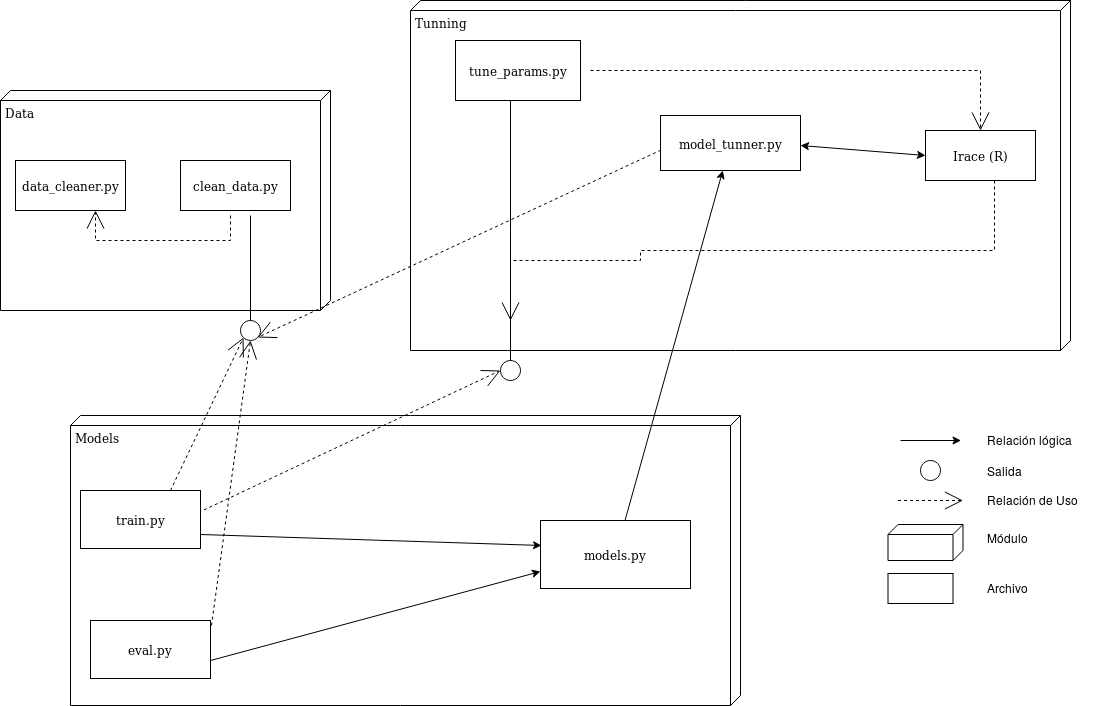
\includegraphics[width=1\textwidth]{images/sistema_modeling_mosquitos}%
          \caption{Sistema para el ajuste de parámetros y modelado}\label{fig:sistema_modelado}
          \end{figure}

        \par En el módulo \verb|data|, como se puede deducir de su nombre,
          es el que encargado de limpiar los conjuntos de datos y generar los
          bloques de entrenamiento, validación y las instancias para realizar
          el ajuste de hiperparámetros de cada algoritmo.

        \par \verb|models| es el módulo dedicado a definir los algoritmos y
          posee los \textit{scripts} para el entrenamiento y
          evaluación de los mismos. Sumado a ésto, en este modulo se encuentra
          el archivo donde se deben colocar los modelos que serán utilizados
          en el modelado.

        \par \verb|tunning| es el módulo encargado del ajuste de hiperparámetros
          de los modelos. Éste realizará una búsqueda sobre el espacio de
          parámetros para encontrar los óptimos para cada algoritmo. Este
          procedimiento utiliza la herramienta \textit{irace} del lenguaje
          \textit{R} desde una interfaz de \textit{Python}.

      \subsubsection{Detalles de código}

        \par Se decidió realizar todo el desarrollo en el lenguaje de programación
          \textit{Python} por su simplicidad, buen desempeño y su extensa
          comunidad activa. Esto facilita el desarrollo, incrementa la velocidad
          de producción y, como un factor muy importante, también permite
          una usabilidad amena de usuario final. El proyecto está disponible
          en \url{https://github.com/juansca/modeling-mosquitos} y en su sección
          inicial se pueden encontrar instrucciones para su instalación.
          A continuación se describirán
          algunos detalles que se consideran importante de los distintos módulos,
          sin entrar en cuestiones irrelevantes.

        \par El módulo \verb|data| por un lado tiene un archivo llamado
          \verb|constants.py| en donde se definen algunas constantes que
          son dependientes del conjunto de datos que se utilizará. Es importante
          dado que es allí en donde se especifican los \textit{features} (o
          columnas) que se utilizarán como input para predicción.
          A su vez, en dicho módulo, el archivo \verb|data_cleaner.py|
          posee una clase llamada \verb|DataCleaner| que es la encargada de
          realizar la limpieza de los datos. Para realizar la limpieza de los
          datos se debe ejecutar el script \verb|scripts/clean_data.py|, el
          cual arroja el siguiente instructivo:

          \begin{lstlisting}
          $ python data/scripts/clean_data.py --help

          Clean Data.

          Usage:
            ./clean_data.py -i <file> -o <dir> [--p_eval <float>] [--instances <n>] [--overlap <f>]

          Options:
            -i <file>              Evaluate dataset path
            -o <dir>               Directory where the evaluation plot result will be
                                   saved
            --p_eval <float>       Percentage to evaluation dataset. [default: 0.2]
            --instances <n>        Number of instances to generate from data
                                   [default: 1]
            --overlap <f>          Percentage of overlapping between the instances.
                                   [default: 0]

          \end{lstlisting}


        \par Por otro lado, el módulo \verb|models| tiene un archivo llamado
          \verb|models.py| en el cual se declaran los modelos
          que se utilizarán para el modelado. Es importante que estos modelos
          sigan la estructura ahí utilizada para que los demás módulos los
          puedan utilizar correctamente.

        \par Además, allí se encuentra el \textit{script} de entrenamiento,
          \verb|scripts/train.py|, que entrena el modelo elegido con el conjunto
          de datos dado e imprime por linea de comandos un conjunto de
          estadísticas que resultan de realizar validación cruzada sobre
          los datos brindados por el usuario para dicha tarea. Ésto resulta útil
          para tener una noción del desempeño del modelo.
          Éste script devuelve la siguiente documentación de uso:
          \begin{lstlisting}
          $ python models/scripts/train.py --help

          Train a model

          Usage:
            ./train.py -i <file> --model <model> [-p <file>]
            ./train.py -h | --help

          Options:
            -i <file>         Train/Val dataset path
            --model <model>   Model you want to train, is mandatory that it was on
                              models.py file.
            -p <file>         CSV file where are saved the hyperparameters
                              (in case of tunning module was used).
          \end{lstlisting}

        \par Por otra parte, el módulo posee un \textit{script} de evaluación,
        que, además de imprimir por linea de comandos el valor del Error Cuadrático Medio de la
        evaluación, genera un gráfico con la curva real y la curva predicha
        por el modelo y lo guarda en un directorio. A su vez, guarda un
        archivo \verb|csv| con los valores reales y los generados por el modelo
        facilitando así, la posterior manipulación del mismo.
        La documentación de ayuda para su utilización es:
        \begin{lstlisting}
        $ python models/scripts/eval.py --help

        Evaluate a model

        Usage:
          ./eval.py -i <file> -m <model> [-o <file>]

        Options:
          -i <file>         Evaluate dataset path
          -m <model>        Model you want to evaluate as pickle format
          -o <dir>          Directory where the evaluation plot result will be saved

        \end{lstlisting}

      \par Finalmente, el sistema desarrollado posee el módulo \verb|tunning|.
        Allí se realiza el ajuste de hiperparámetros de los modelos.
        Existe varios archivos en ese módulo que son los que hacen de interfaz
        con la herramienta \textit{irace}. Algo que cabe destacar aquí es el
        directorio \verb|parameters|. Allí se colocan los posibles
        (o intervalos de) valores que generan el espacio de hiperparámetros
        donde la herramienta buscará los óptimos para cada modelo. Además,
        \textit{irace}, usará las instancias de datos en \verb|instances|
        para realizar dicha tarea. Algo de suma importancia es que
        los datos utilizados para generar los últimos conjutos deben ser distintos
        a los que se usarán posteriormente en el entrenamiento o validación de
        los modelos. Esto se debe a que si no, se puede generar una dependencia
        de los datos y podría llevar al sobre-ajuste (\textit{overfitting})\footnote{Una
        analogía clara es que el modelo aprende "de memoria" los datos en vez de
        comprenderlos. Esto lleva a una muy pobre capacidad de generalización.}.
        El \textit{script} que se debe ejecutar para hacerlo es \verb|tune_params.py|.
        Su documentación de uso es:
        \begin{lstlisting}
        $ python tunning/tune_params.py --help

        Tune parameters for given models.

        Usage:
          tune_params.py --model <name>

        Options:
          --model <name>           model name to tune params.
                                   Options: svr, rdmforest, pcardmforest, dtr, knnr,
                                   mlpr, svr, pcaknnr, pcadtr.
                                   If you want to tune all the models together, just
                                   put on this parameter 'all'.
          --help                   show this screen

        \end{lstlisting}
      \par Por último, en la Figura \ref{fig:proyecto_modelado} se puede observar
        la estructura general del proyecto.

        \begin{figure}[hbt]
        \centering%
        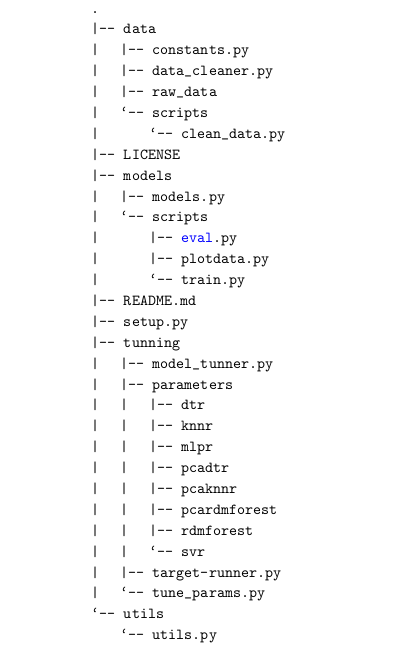
\includegraphics[width=0.6\textwidth]{images/proyecto_modeling}%
        \caption{Sistema para el ajuste de parámetros y modelado}\label{fig:proyecto_modelado}
        \end{figure}



    \subsection{Modelos lineales}

      \par Experiencias previas en aplicaciones epidemiológicas de
        modelado utilizando variables ambientales obtenidas de sensores
        remotos han reportado buenos resultados con éste
        enfoque \cite{akodon_modeling, multilinear_apli, modis_data}.
        En este caso se utilizó un modelo de regresión lineal tradicional y
        una regresión \textit{Ridge}, esta última con la regularización de
        \textit{Tikhonov} y validación cruzada. Cabe destacar que la
        regresión \textit{Ridge}, en la literatura de ML, se la suele denominar
        como "decaimiento de peso" (\textit{weight decay}).

  \subsection{Modelos no-lineales}

    \par A diferencia de los modelos lineales, los no-lineales son capaces de
      capturar relaciones funcionales más complejas entre los datos, con el costo
      de una complejidad computacional más grande y una carga mucho mayor para el
      usuario que debe realizar un trabajo más fino de ajuste del modelo (la
      selección de hiperparámetros, entre otras).

    \par Tipicamente, una regresión en el ámbito del aprendizaje automático
      incluye cuatro pasos fundamentales:
      \begin{itemize}
        \item Análisis del conjunto de datos: implica extraer variables de interés, quitar redundacia y valores que generen
              ruido, etc
        \item Arquitectura: Selección del algoritmo y de los hiperparámetros como
              la cantidad de capas y neuronas en una ANN, el número de vecinos en
              el algoritmo de K-vecinos más cercanos, etc.
        \item La etapa de entrenamiento-validación: los parámetros del modelo
              se ajustan y se realizan técnicas de validación de dicho modelo para
              medir el desempeño del modelo para generalizar a nuevos datos.
        \item Utilizar el modelo con datos nuevos.
      \end{itemize}
      Éstos pasos se implementaron utiliizando, mayormente, funciones disponibles
      en la librería \textit{scikit-learn} ya mencionada.

    \par La configuración o selección del conjunto óptimo de hiperparámetros
      en este tipo de modelos no-lineales es un problema complejo. Ésto
      podría realizarse a mano utilizando herramientas semi automáticas. Lo primero
      no es buena práctica dado que podría generar un sesgo sobre los valores
      obtenidos y, además, el gran número de posibles combinaciones requeriría
      mucho tiempo del usuario en ésta tarea, aún así hay ocasiones en las
      que se utiliza esta metodología.

    \par Para realizar el ajuste de hiperparámetros, en este trabajo para la
      utilizó el paquete \textbf{\textit{IRace}}
      (\textit{Iterated Racing for Automatic Algorithm Configuration}) \cite{irace}.
      Ésta herramienta realiza un procedimiento iterativo capaz de encontrar
      automáticamente la configuración de hiperparámetros más apropiada
      dadas las instancias de datos generadas para esta etapa.
      Ésta está disponible gratuitamente para el lenguaje \textbf{R} en
      \url{http://iridia.ulb.ac.be/irace/}.

    \par Para evitar el sobre-entrenamiento (\textit{overfitting}), el ajute
      fue hecho automáticamente con datos de otras ciudades: Clorinda, Iguazú
      y Pampa.


    \subsubsection{\textit{Support Vector Regressor} (SVR)}
      \par Las \textit{Support Vector MAchines} son una clase de técnica supervisada
        que construyen tanto reglas de decisiones lineales como no-lineales
        y modelos de regresión. En este caso se utilizó el algoritmo \verb|SVR|
        del módulo \verb|SVM|. Éste método implementa una regresión
        \textit{Epsilon-Support Vector}. Luego de la etapa de ajuste de
        hiperparámetros, el valor para la penalidad es de $C = 0.887453$, y
        el núcleo de función de base radial (RBF) con un valor de
        $gamma = 0.015561$.


    \subsubsection{\textit{Perceptron Multicapa} (MLP)}
      \par Las redes neuronales son contruidas a partir de una gran cantidad
        de unidades sencillas altamente conectadas entre si. Ellas pueden
        ser entrenadas para generar aproximadores universales de funciones.
        Se utilizó la clase \verb|MLPRegressor| del módulo \verb|neural\_network|.
        Ésta clase implementa una técnica de regresión utilizando un MLP. Para
        ello optimiza el error cuadrático utilizando el \textit{LBFGS} y
        el descenso estocástico por grandiente.
        Luego de la etapa de ajuste, se obtuvo un valor para el término
        de regularización cuadrática de $alpha = 0.070921$, y un total de
        tres capas y con tres neuronas cada unas completan la arquitectura
        del modelo. La activación es hecha por la función lineal
        rectificada $f(x) = max\{0, x\}$.


    \subsubsection{Regresión de K-Vecinos Más Cercanos (KNNR)}
      \par Se utilizó la clase \verb|K-NeighborsRegressor|. Este método
        infiere una regresión basada en los k-vecinos más cercanos. El
        objetivo es predicho por una interpolación local de los objetivos
        en el entorno de vecinos del conjunto de datos de entrenamiento.
        El cojunto de datos original se descompuso utilizando componentes
        principales (\textit{PCA}), sólo cinco fueron usados. Luego de la etapa
        de ajuste, se obtuvo que el número de vecinos sea $n\_neighbors = 4$,
        la función de pesos utilizada en predicción que resultó generar mejor
        desempeño fue $weights = uniform$, la métrica utilizada para medir la
        distancia fue $metric = Chebyshev$ y el algoritmo que nuestro modelo
        utiliza para calcular los vecinos más cercanos resultó ser
        $algorithm = ``brute"$.

    \subsubsection{Regresión de Árboles de Decisión (DTR)}
      \par Los árboles de decisión son reglas de clasificación construidas de
      forma incremental, a partir de las cuales se puede aprender un modelo
      de regresión. En este trabajo se utilizó la clase \verb|K-NeighborsRegressor|
      del módulo \verb|tree|. Nuevamente, se utilizó \textit{PCA} pero, esta
      vez, se conservaron sólo los dos primeros componentes. Además, luego de
      dicha etapa se concluye que la regla de división sea $splitter = ``best"$,
      el valor máximo para la profundida del árbol $max_depth = 3$ y el mínimo
      valor de muestras requeridas para dividir un nodo interno es
      $min\_samples\_leaf = 5$.

      \par La elección del número de componentes en el \textit{PCA} para los
      dos últimos métodos fue basada en prueba y error, buscando por el
      subconjunto más pequeño que produzca buenos resultados.


  \section{Resultados}
    \begin{figure}[hbt]
    \centering%
    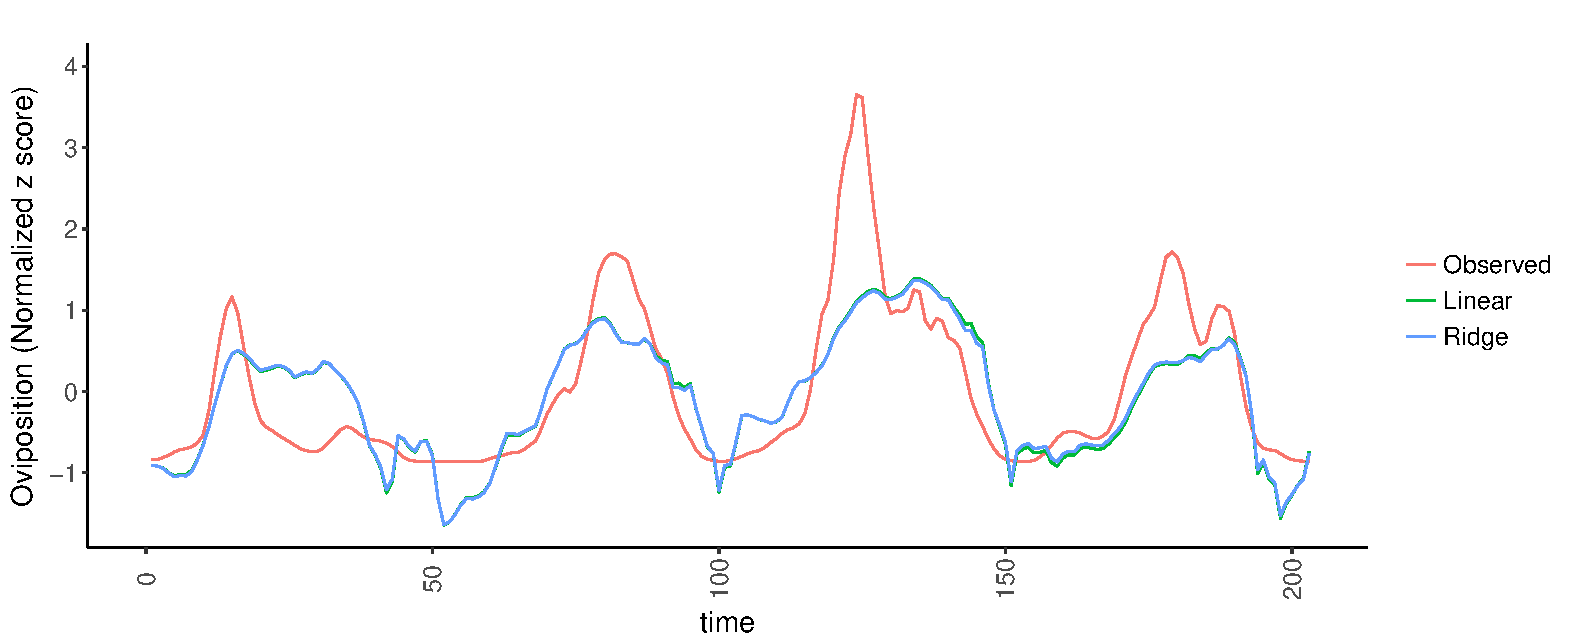
\includegraphics[width=1\textwidth]{images/RidgeVsTime}%
    \caption{\textit{Z-score} observado, regresiones lineales tradicional y
             \textit{Ridge}}\label{fig:ridge_vs_time}
    \end{figure}

    \par La Figura \ref{fig:ridge_vs_time} muestra los resultados tanto del
      modelo lineal clásico como el \textit{Ridge}. Estos resultados concuerdan
      con estudios previos. Ambos regresores lineales producen resultados muy
      similares, por lo que resulta evidente que es preferible utilizar el
      primero debido al menor costo computacional que requiere.
      \begin{figure}[hbt]
      \centering%
      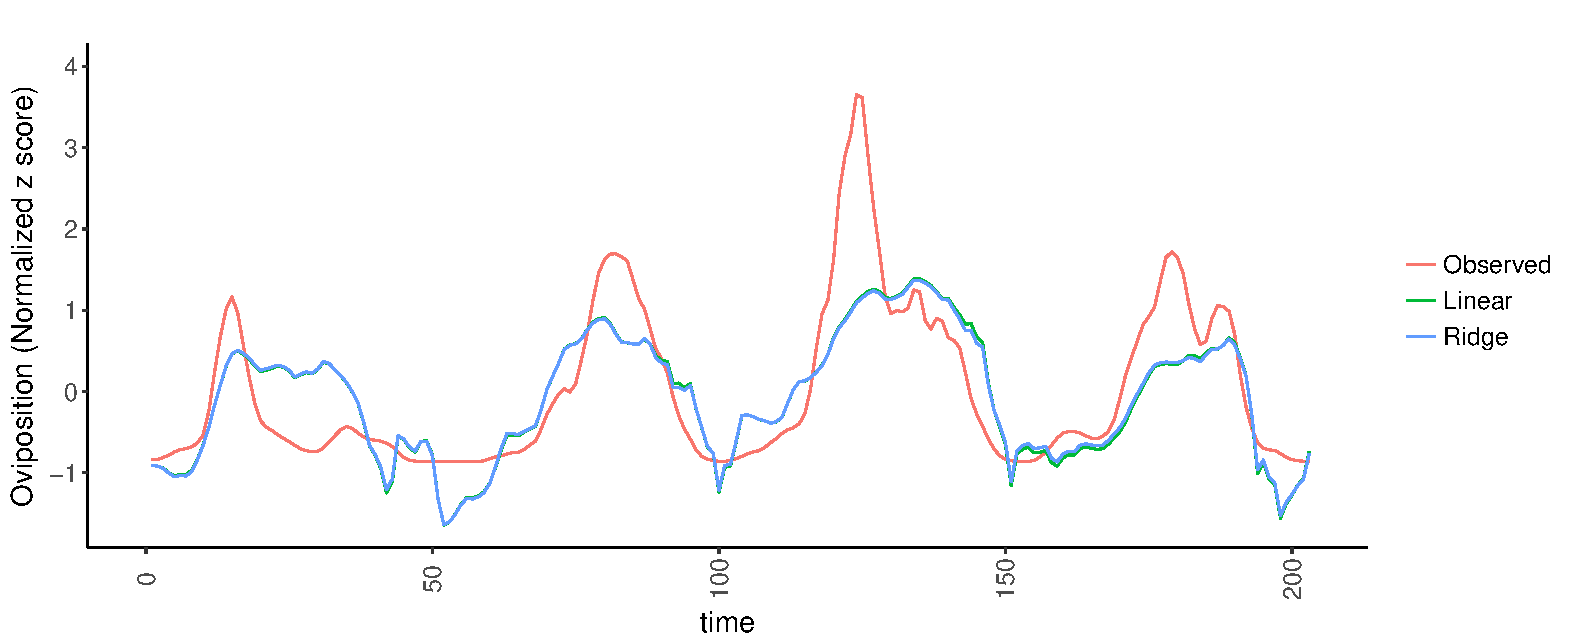
\includegraphics[width=0.9\textwidth]{images/RidgeVsTime}%
      \caption{\textit{Z-score} observado, regresiones lineales tradicional y
               \textit{Ridge}}\label{fig:ridge_vs_time}
      \end{figure}

    \par Los regresores lineales no se adecúan a los picos de los datos
    observados, y tienden a subestimar los valor más pequeños.

    \par La Figura \ref{fig:svr} muestra los datos observados y el resultado
      del procedimiento de regresión por \textit{SVR}. Éste último no modela los
      picos de los primeros, pero si produce un ajuste relativamente bueno
      en la mayor parte de los datos.
      \begin{figure}[hbt]
      \centering%
      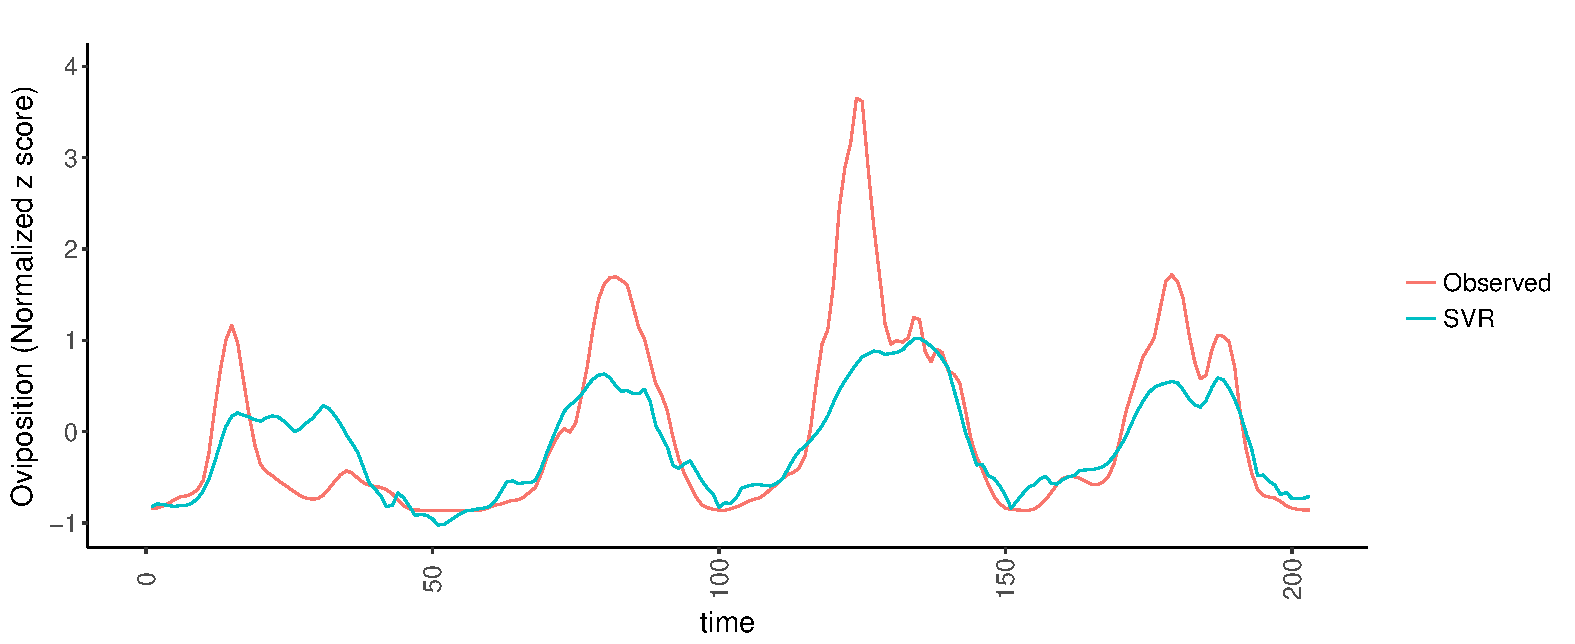
\includegraphics[width=0.9\textwidth]{images/svr}%
      \caption{\textit{Z-score} observado y regresión SVR}\label{fig:svr}
      \end{figure}


    \par La Figura \ref{fig:mlp} muestra los resultados del ajuste de
    los datos observados utilizando la técnica de \textit{MLP}. Dicho ajuste es muy
    bueno, aunque el modelo sobreestima los datos alrededor de la semana 25
    del estudio, y los subestima alrededor del último pico.
      \begin{figure}[hbt]
      \centering%
      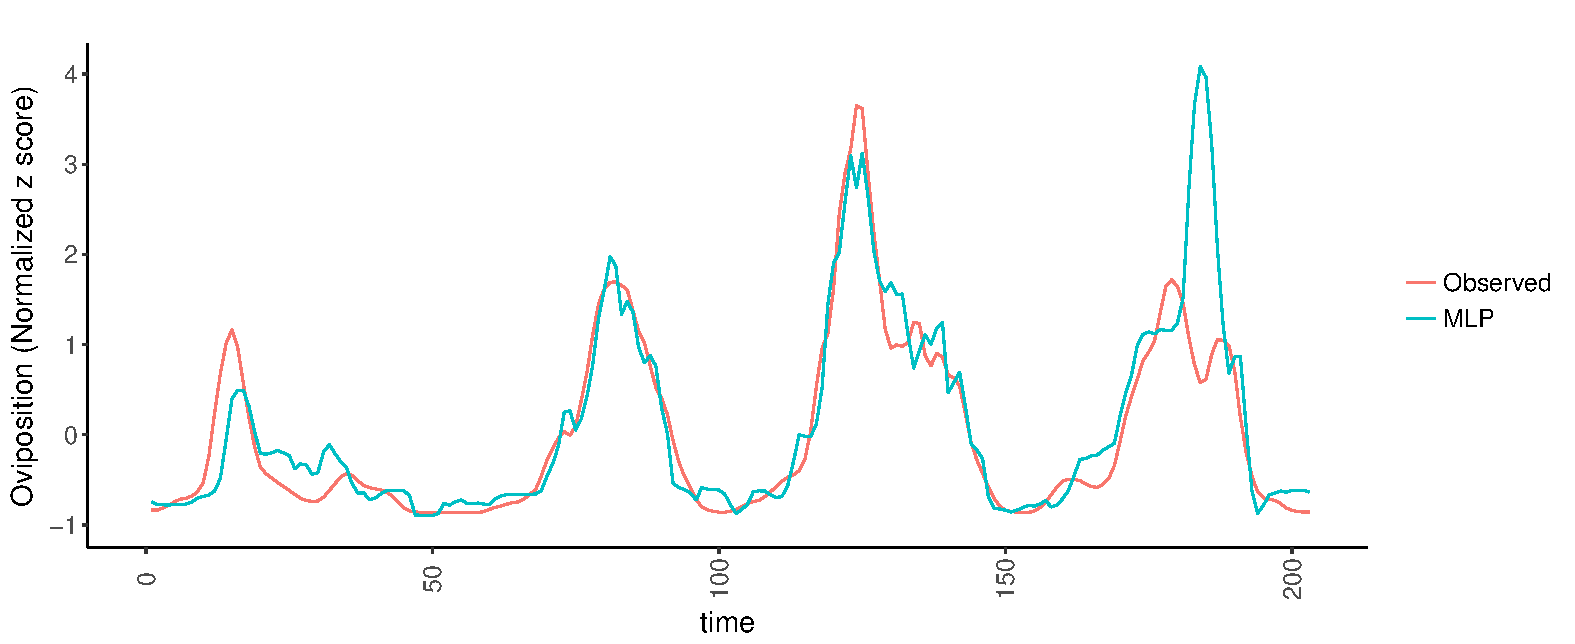
\includegraphics[width=0.9\textwidth]{images/mlp}%
      \caption{\textit{Z-score} observado y regresión MLP}\label{fig:mlp}
      \end{figure}


  \par La Figura \ref{fig:knn} muestra los resultados producidos por el procedimiento
    de \textit{KNN}. Se observa que, también, este modelo es muy bueno aunque
    falla siguiendo a los dos picos más altos. El primero, alrededor de la semana
    125 es subestimado, y el segundo, que está cerca de la semana 180, es
    sobreestimado.

    \begin{figure}[hbt]
    \centering%
    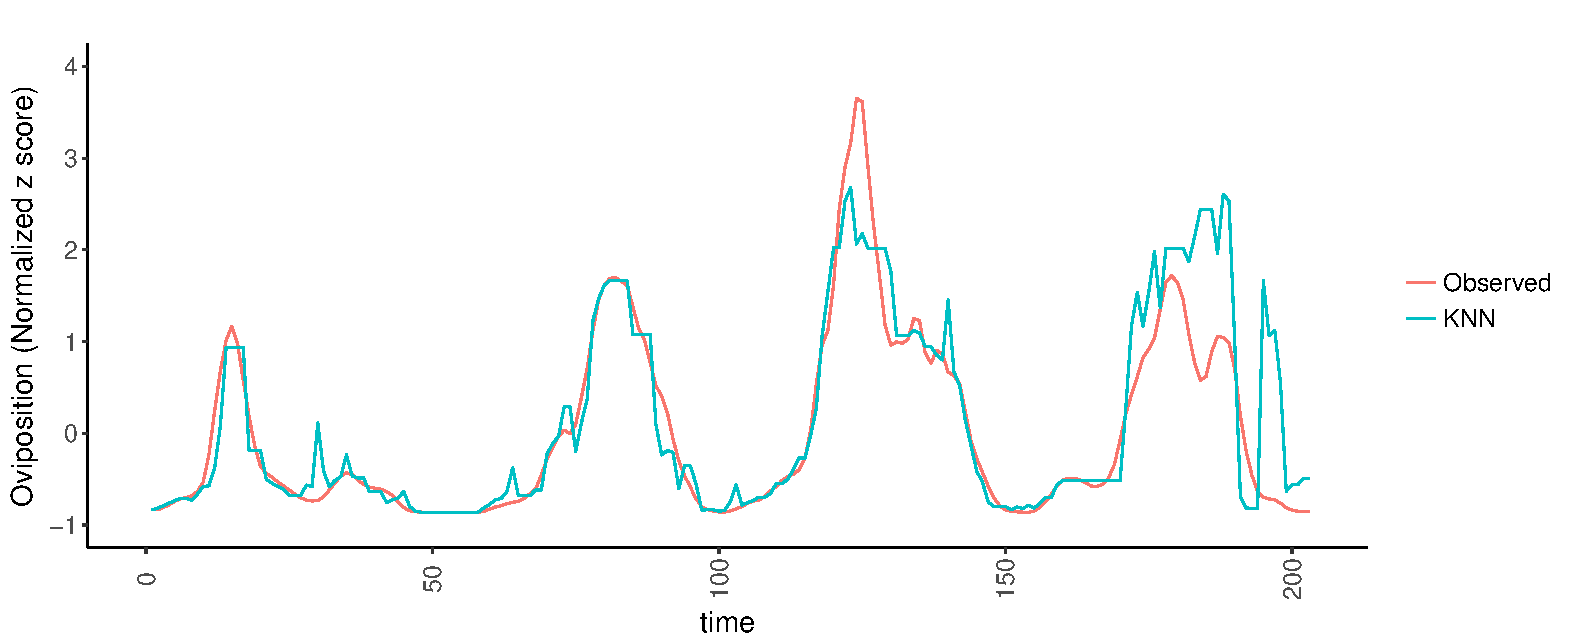
\includegraphics[width=0.9\textwidth]{images/knn}%
    \caption{\textit{Z-score} observado y regresión KNN}\label{fig:knn}
    \end{figure}


  \par La Figura \ref{fig:dtr} muestra el resultado de aplicar \textit{DTR}.
    La estructura de este procedimiento produce salidas
    planas que, sin embargo, siguen de cerca los datos observados.
    Es importante recordar que en todas las figuras anteriores, las últimas
    40 semanas no fueron utilizadas para construir los modelos, por lo que
    han sido completamente predichas.

    \begin{figure}[hbt]
    \centering%
    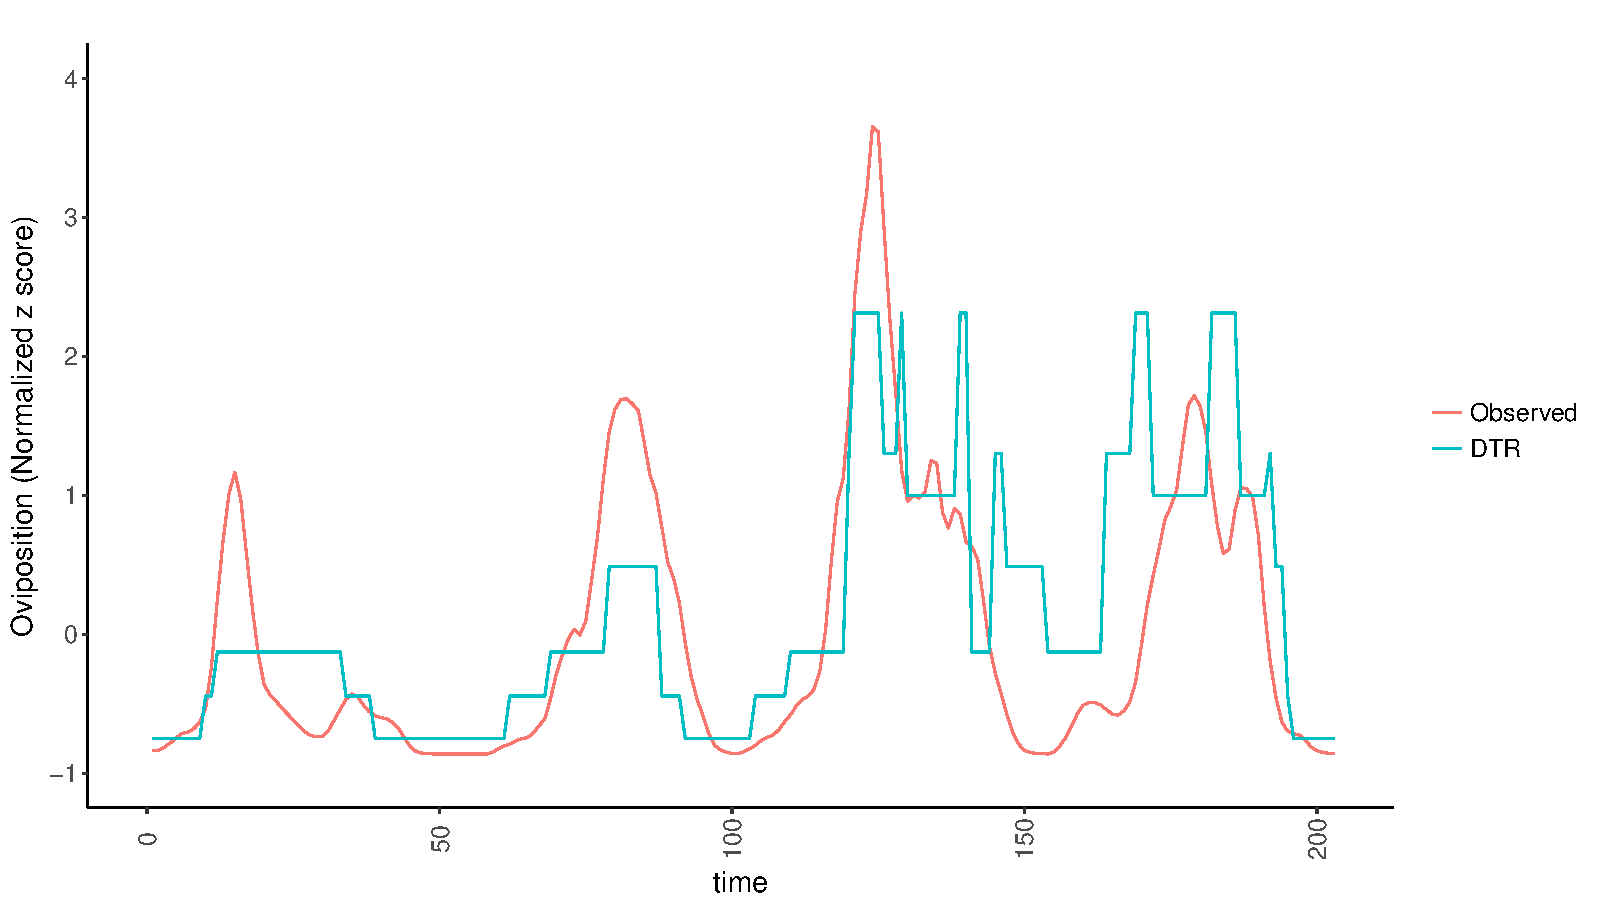
\includegraphics[width=0.9\textwidth]{images/dtr}%
    \caption{\textit{Z-score} observado y regresión DTR}\label{fig:dtr}
    \end{figure}



  \par La tabla \ref{Tab:Summary} presenta un resumen de los datos obsevados
    y los ajustados: los valores minimos (Min) y los máximos (Max), el
    primer ($q_{1/4}$) y tercer cuartil ($q_{3/4}$), la mediana ($q_{2/4}$)
    y la media.

  \begin{table}[hbt]
  \centering
  \caption{Resumen de los datos observados y los ajustados}\label{Tab:Summary}
  \begin{tabular}{*7{r}}
  \toprule
  &Min	&$q_{1/4}$	&$q_{1/2}$	&Media	&$q_{3/4}$	&Max\\ \cmidrule(lr){2-7}
  Observado	&$-0.863$	&$-0.742$	&$-0.487$	&$0.000$	&$0.704$	&$3.652$\\
  Lineal	&$-1.641$	&$-0.716$	&$ 0.027$	&$-0.087$	&$0.462$	&$1.387$\\
  Ridge	&$-1.638$	&$-0.680$	&$ 0.028$	&$-0.084$	&$0.459$	&$1.370$\\
  MLP	&$-0.894$	&$-0.677$	&$-0.323$	&$0.093$	&$0.716$	&$4.084$\\
  DTR	&$-0.752$	&$-0.752$	&$-0.128$	&$0.138$	&$0.998$	&$2.312$\\
  KNNR	&$-0.863$	&$-0.699$	&$-0.501$	&$0.099$	&$1.033$	&$2.679$\\
  SVR	&$-1.021$	&$-0.601$	&$-0.232$	&$-0.147$	&$0.309$	&$1.023$\\
  \bottomrule
  \end{tabular}
  \end{table}

  \par La Tabla \ref{Tab:Summary} revela los siguientes hechos:

    \begin{itemize}
      \item Las regresiones lineal y \textit{Ridge} exageran los minimos, ya
        que producen valores que son aproximadamente el doble que los observados.
      \item El Perceptron Multicapa exagera el máximo por alrededor de un \SI{10}{\percent},
        mientras que los otros modelos subestiman dicho valor. Notar que el \textit{SVR}
        aplana el máximo por un factor de aproximadamente 3.6.
      \item La media y mediana observadas difieren notablemente, sugiriendo que
        los modelos están significativamente sesgados a la izquierda.
      \item El valor más cercano al observado, de la mediana, es producido por
        \textit{KNN}, el cual también conduce a un valor cercado de la media.

    \end{itemize}


    \par La Figura \ref{fig:scatter} muestra los datos observados y predichos
      como un \textit{scatterplot}. Esta figura revela que ninguno de los modelos
      es capaz de seguir los valores más grandes observados, y que los modelos
      Lineal, \textit{Ridge} y \textit{SVR} son los menos aptos para esta
      tarea, mientras que \textit{MLP} es la más adecuada. Además se notó que
      este último modelo es el más propenso a sobreestimar los datos. Cabe
      destacar que la subestimación es, para el punto de vista de la aplicación,
      más peligroso que la sobreestimación, dado que el primero tiende a
      ser un falso indicador negativo que puede llevar a no disparar medidas
      de prevención en casos en que efectivamente se necesiten.
      \begin{figure}[hbt]
      \centering%
      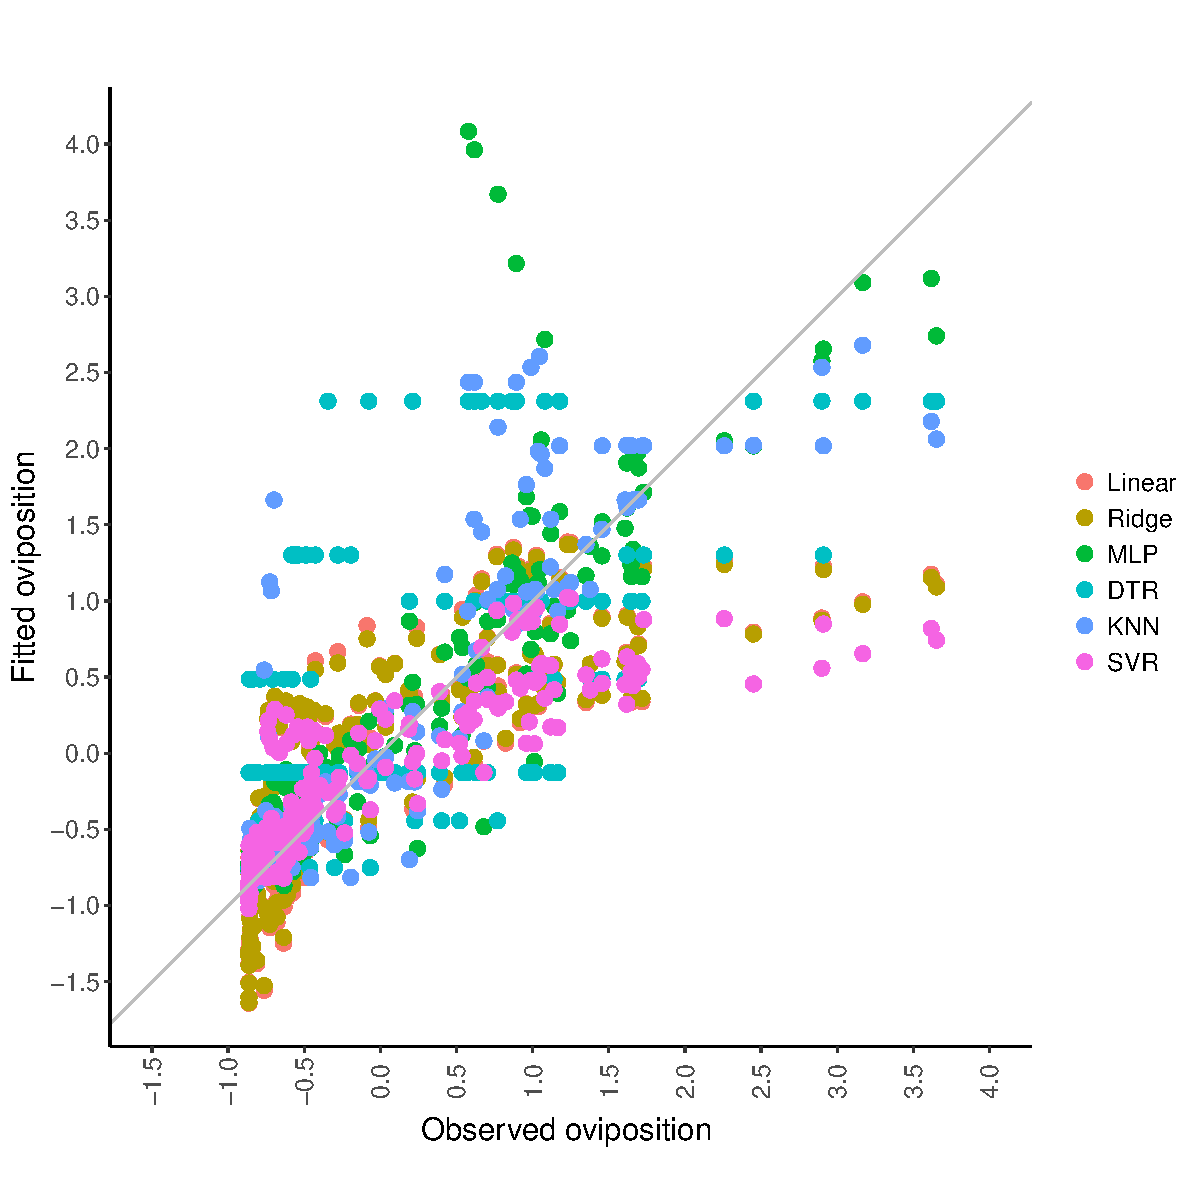
\includegraphics[width=0.6\textwidth]{images/scatterplot}%
      \caption{Scatterplot de los valores observados y predichos}\label{fig:scatter}
      \end{figure}



    \par A continuación se analizará los errores. Las Figuras \ref{fig:Histograms}
    y \ref{fig:Boxplots} muestran, respectivamente, los histogramas y boxplots
    de los errores producidos por cada modelo. Los errores generados por
    \textit{KNN} son los más concentrados alrededor de cero, seguidos por el
    \textit{MLP}. Los dos errores más extendidos son se corresponden con
    las regresiones lineales. Éste es un indicador de que los modelos
    obotenidos utilizando simples técnicas lineales son los peores entre los
    considerados en este trabajo.
      \begin{figure}
      \centering
      \subfigure[Histogramas\label{fig:Histograms}]{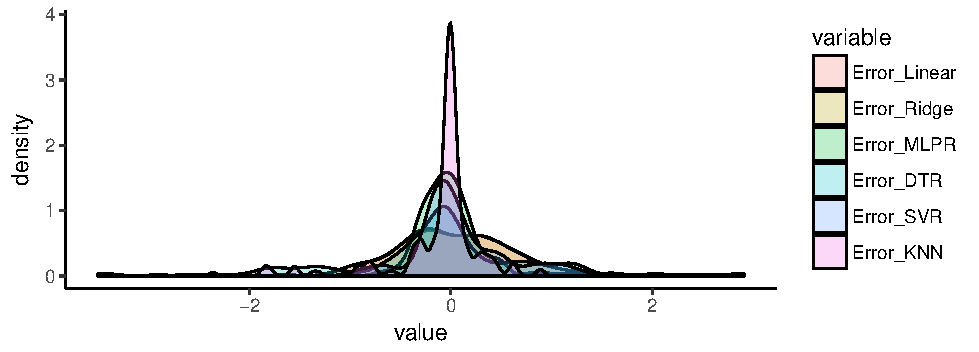
\includegraphics[width=.8\linewidth]{images/histogram_error}}
      \subfigure[Boxplots\label{fig:Boxplots}]{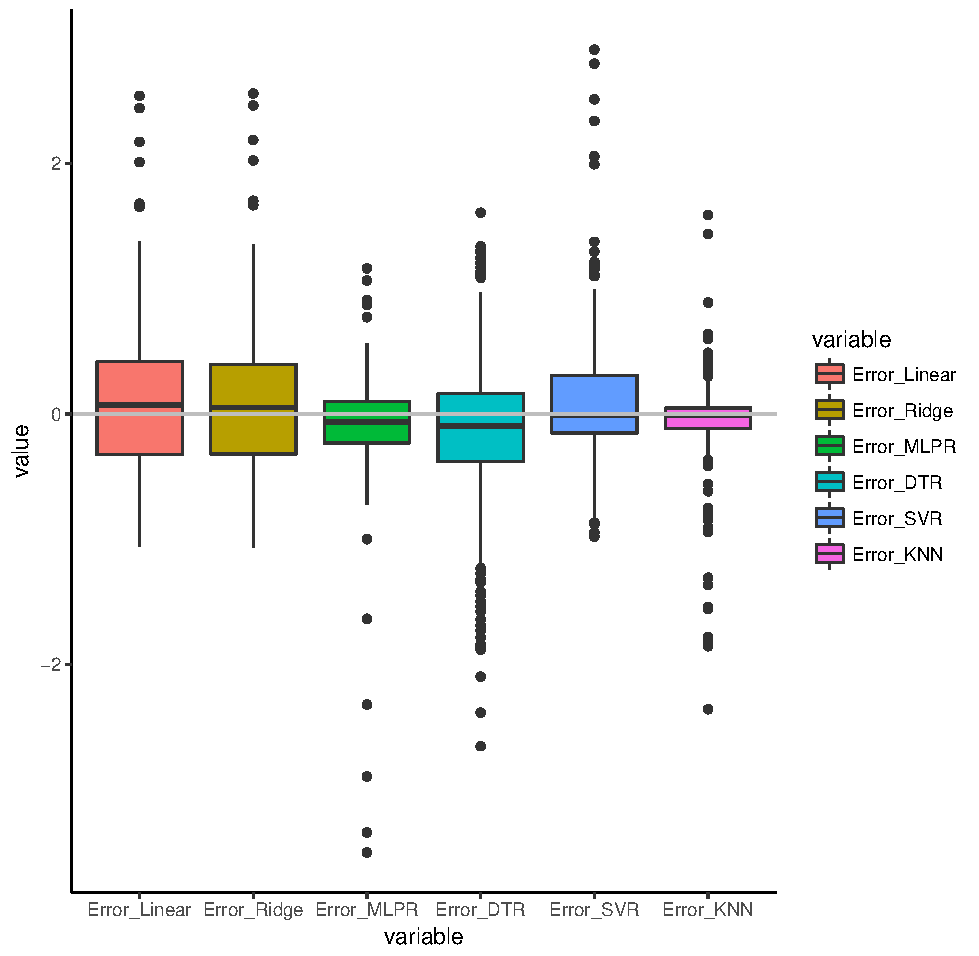
\includegraphics[width=.8\linewidth]{images/boxplot_error}}
      \caption{Errores}\label{fig:Residuals}
      \end{figure}


  \par La Tabla \ref{Tab:Quality} presenta las medidas de calidad de los modelos
  aquí considerados: los coeficientes de la correlación de \textit{Pearson}
  entre los valores observados y ajustados, usando el conjunto de datos
  completo (Corr11) y sobre el 20\% para la validación (CorrL20); además,
  el Error Cuadrático Medio sobre el conjunto de datos completo (MSE), y
  sólo sobre los datos de validación (MSEL20). Siguiendo \cite{dynamics_of_dengue},
  también se incluyó el \textit{z-score} medio obtenido de la validación
  cruzada y su desviación estándar (SD del Z-Score).


  \begin{table}[hbt]
  \centering
  \caption{Medidas de calidad de los modelos}\label{Tab:Quality}
  \begin{tabular}{*7{r}}
  \toprule
  & Corr11
  & MSE
  & Z-Score Medio
  & SD del Z-Score
  & CorrL20
  & MSEL20 \\ \midrule
  Lineal
  &$0.774$
  &$0.624$
  &$1.108$%&\boldmath$1.108$  %CARO: cambio
  &$0.278$
  &$0.890$
  &$0.580$\\
  Ridge
  &$0.775$
  &$0.621$
  &$1.072$
  &$0.277$
  &$0.896$
  &$0.566$ \\
  SVR
  &$0.837$
  &$0.613$
  &\boldmath$0.834$   %CARO: cambio
  &$0.490$
  &\boldmath$0.967$
  &\boldmath$0.464$ \\
  MLP
  &$0.875$
  &$0.528$
  &$1.086$
  &$0.288$
  &$0.727$
  &$1.023$ \\
  KNN
  &\boldmath$0.888$
  &\boldmath$0.494$
  &$0.981$
  &$0.362$
  &$0.797$
  &$0.936$\\
  DTR
  &$0.679$
  &$0.768$
  &$1.148$
  &$0.544$
  &$0.532$
  &$1.131$ \\
  \bottomrule
  \end{tabular}
  \end{table}

  \section{Conlusiones}

    \par Un punto interesante que aparece en los resultados es que todos los
      modelos aquí presentados ajustan bien en los patrones principales
      pero no necesariamente en los picos extremos. Una hipótesis es que la población
      del vector se desconecta de las variables macroambientales/climáticas
      cuando las condiciones son óptimas y, nuevamente, se restringe cuando las
      condiciones ambientales son suboptimas. De hecho, es razonable el hecho de
      que no podemos esperar ajustar exactamente la población urbana del vector
      sólo basandonos en variables macroambientales a gran escala.


    \par Teniendo en cuenta la bondad de ajuste incluida en las Tablas
      \ref{Tab:Summary} y \ref{Tab:Quality}, y un análisis de errores, podríamos
      considerar que \textit{KNN} aparenta ser el mejor método para este problema.
      Tiene una correlación cercana al 90\%, considerablemente mayor al
      75\%, el valor tipico obtenido por las técnicas lineales.

  \par El valor medio del \textit{z-score} llevaría a elegir el \textit{SVR}
    como la mejor técnica \cite{ml_rainfall}. Cabe destacar que la desviación
    estándar de esta medición de calidad es tan alta que es poco probable que
    sea una buena elección en si misma. Por esta razón, se seguimos un
    enfoque holístico en las próximas conclusiones.


  \par Si tenemos en cuenta las seis métricas de la Tabla \ref{Tab:Quality},
    es clara la conclusión de que los mejores métodos para modelar la población
    del vector basada en variables ambientales derivadas de información satelital
    son: \textit{K-vecinos más cercanos}, \textit{Perceptron
    Multicapa} y \textit{Support Vector Machine}.

  \par Un problema que encontramos es la escases de datos de campo que existen:
    el desempeño de estos algoritmos se podría mejorar sustancialmente utilizando
    conjuntos de datos más grandes.
    Aunque el período utilizado es grande en comparación con trabajos similares
    sobre la población vectorial, dicho conjunto sigue siendo
    muy pequeño desde el punto de vista del aprendizaje automático.

  \par Otro problema, no menos importante teniendo en cuenta el objetivo final
    de los esfuerzos puestos en este sentido (tener modelos operativos de
    riesgo), es la gran escases de puntos (ciudades) de los cuales se posee información
    de campo (oviposición). Esto resulta un problema dado que si los modelos son
    entrenados con datos de un punto geográfico \textbf{A} (Tartagal, por ejemplo), a
    priori no podemos aseegurar que serán capaces de ajustar correctamente al
    comportamiento de la variable objetivo de un punto \textbf{B} (Córdoba, por ejemplo).
    Pues ni siquiera se poseen datos para validar dicha conducta.
    Esto limita el alcance regional de las herramientas de este tipo.


  \par Como comentario final de este capítulo queremos mencionar que el trabajo
    realizado y descripto aquí ha llevado a la publicación del trabajo
    \textit{Modeling Dengue Vector Population Using Remotely Sensed Data and
    Machine Learning} \cite{scavuzzo2018modeling} en la revista \textit{Acta Tropica}
    de \textit{Elsevier} (\url{https://www.journals.elsevier.com/acta-tropica}).

\end{document}

%\documentclass[12pt,spanish,fleqn,openany,letterpaper,pagesize]{scrbook}

\usepackage[utf8]{inputenc}
\usepackage[spanish]{babel}
\usepackage{fancyhdr}
\usepackage{epsfig}
\usepackage{epic}
\usepackage{eepic}
\usepackage{amsmath}
\usepackage{threeparttable}
\usepackage{amscd}
\usepackage{here}
\usepackage{graphicx}
\usepackage{lscape}
\usepackage{tabularx}
\usepackage{subfigure}
\usepackage{longtable}


\usepackage{rotating} %Para rotar texto, objetos y tablas seite. No se ve en DVI solo en PS. Seite 328 Hundebuch
                        %se usa junto con \rotate, \sidewidestable ....


\renewcommand{\theequation}{\thechapter-\arabic{equation}}
\renewcommand{\thefigure}{\textbf{\thechapter-\arabic{figure}}}
\renewcommand{\thetable}{\textbf{\thechapter-\arabic{table}}}


\pagestyle{fancyplain}%\addtolength{\headwidth}{\marginparwidth}
\textheight22.5cm \topmargin0cm \textwidth16.5cm
\oddsidemargin0.5cm \evensidemargin-0.5cm%
\renewcommand{\chaptermark}[1]{\markboth{\thechapter\; #1}{}}
\renewcommand{\sectionmark}[1]{\markright{\thesection\; #1}}
\lhead[\fancyplain{}{\thepage}]{\fancyplain{}{\rightmark}}
\rhead[\fancyplain{}{\leftmark}]{\fancyplain{}{\thepage}}
\fancyfoot{}
\thispagestyle{fancy}%


\addtolength{\headwidth}{0cm}
\unitlength1mm %Define la unidad LE para Figuras
\mathindent0cm %Define la distancia de las formulas al texto,  fleqn las descentra
\marginparwidth0cm
\parindent0cm %Define la distancia de la primera linea de un parrafo a la margen

%Para tablas,  redefine el backschlash en tablas donde se define la posici\'{o}n del texto en las
%casillas (con \centering \raggedright o \raggedleft)
\newcommand{\PreserveBackslash}[1]{\let\temp=\\#1\let\\=\temp}
\let\PBS=\PreserveBackslash

%Espacio entre lineas
\renewcommand{\baselinestretch}{1.1}

%Neuer Befehl f\"{u}r die Tabelle Eigenschaften der Aktivkohlen
\newcommand{\arr}[1]{\raisebox{1.5ex}[0cm][0cm]{#1}}

%Neue Kommandos
\usepackage{Befehle}


%Trennungsliste
\hyphenation {Reaktor-ab-me-ssun-gen Gas-zu-sa-mmen-set-zung
Raum-gesch-win-dig-keit Durch-fluss Stick-stoff-gemisch
Ad-sorp-tions-tem-pe-ra-tur Klein-schmidt
Kohlen-stoff-Mole-kular-siebe Py-rolysat-aus-beu-te
Trans-port-vor-gan-ge}

%
%\begin{document}
%
\justifying

\chapter{Generalización espacial de modelos epidemiológicos basada en el
        concepto de Distancia Ambiental Normalizada NED}

  \par Los modelos temporales descriptos en capítulos anteriores se basan en la
    generación de relaciones empíricas entre datos ambientales derivados de
    información satelital y los datos de campo, correspondientes a los del vector
    propiamente dicho. Esto significa que sólo pueden construirse modelos en
    lugares donde esté disponible la información de campo, problema que se
    menciona al concluir el capítulo anterior.

  \par En ese marco, y con el objetivo final de mejorar la aplicación operativa
    presentada por Porcasi y colaboradores en 2012 \cite{porcasi_operative},
    en este capítulo se plantea el objetivo específico de generar
    una metodología para espacializar los datos contruidos siguiendo la
    metodología del capítulo anterior, basada en el concepto de
    \textbf{\textit{Distancia Ambiental Normalizada}} (NED).

\section{Descripción del problema}
  \par A partir de la disponibilidad de datos de campo en $N$ localidades
    diferentes, se generan
    $N$ modelos que relacionan la oviposición con variables ambientales
    derivadas de datos satelitales (\textit{lst\_night}, \textit{lst\_day},
    \textit{ndvi}, \textit{ndwi}, \textit{prec}). Por simplicidad, sin pérdida
    de generalidad, supongamos que dichos modelos son lineales:
    \begin{align}
      ovip_{j} = \beta_{j} + \sum{}{coef_{ji} \times envVar_{i}(j)}
    \end{align}
    donde $coef_{ji}$ representa los coeficientes del modelo de la
    ciudad $j$ para la variable $i$, y $envVar_{i}(j)$ representa la variable
    ambiental $i$ evaluada en la posición correspondiente a la ciudad $j$.
    Es decir que para cada ciudad $j$, hay un conjunto diferente de
    coeficientes, que son aquellos que generan un ajuste óptimo de los datos
    disponibles. Aquí se denominan a estos $N$ modelos: $M_{1},\ M_{2},\ \dots,\ M_{N}$.


  \par Así, el problema que se plantea es aquel en el que el modelo se
    debiera utilizar en una nueva ciudad (no incluida en las $N$ anteriores) en
    donde se quiere obtener una estimación de la abundancia del vector; para
    de esa manera, obtener la estimación mencionada para cualquier otra
    ciudad. En particular, en este caso, en la región norte de Argentina donde
    no se disponga de datos de campo.


  \par La idea más simple para extrapolar los modelos obtenidos sería usar,
    para un punto/pueblo adicional localizado en la posición $X$, un modelo $M_{X}$
    igual al modelo conocido de la ciudad más cercana geográficamente (vecino más cercano) es
    decir $M_{X}\ =\ M_{J}$ donde $J$ corresponde a la ciudad más cercana.
    Una mejora a este enfoque, es utilizar un promedio de los $N$ modelos conocidos
    ponderados por el inverso de la distancia de este nuevo punto $X$ a cada una
    de las ciudades $J$ donde se dispone de un modelo. Es decir, el modelo de la
    ciudad más cercana pesará más y el de la más alejada pesará menos, es decir:

    \begin{align}
      M_{X} = \sum{}{\frac{M_{j}}{L_{j}}} \label{Eq:dist}
    \end{align}
    donde $L_{j}$ representa la distancia normalizada de la ciudad $J$ a
    $X$ (en términos de la localización geográfica de la nueva ciudad).


  \par El problema de las soluciones anteriores, es que en realidad es más
    razonable pensar que el comportamiento de la población del vector/mosquito
    en una ciudad en el punto $X$ será más coincidente con una que se encuentre
    en una ciudad que sea más similar \textbf{ambientalmente} y no necesariamente
    con aquella que está más cerca geográficamente. En ese sentido, se debería
    utilizar (en el esquema de vecino más cercano) el modelo de la ciudad $J$
    que posea el medio ambiente más similar al del punto $X$. En otras palabras,
    así como ``más cerca", significa típicamente coordenadas geográficas (o posiciones)
    similares; en el sentido ecológico/ambiental, podemos pensar ``más cerca"
    como
    que sus variables ambientales son similares. De esta forma aparece
    naturalmente el concepto de \textbf{\textit{Distancia Ambiental}}.


\section{Distancia Ambiental Normalizada (NED)}

  \par El concepto de \textbf{Distancia Ambiental}, si bien no es completamente nuevo,
    no ha sido utilizado en el contexto de la epidemiología. Una revisión
    exhaustiva de bases de datos bibliográficas de revistas indexadas nos
    arroja que sólo existen 11 publicaciones con ``\textit{Environmental Distance}”
    en su título. El más citado de éstos, es el trabajo de Hirzel \cite{hirzel_distance}
    quien utiliza esta idea en el contexto del estudio de ecología y
    distribución de especies.

  \par Con un enfoque similar, podemos encontrar las contribuciones de Krasnova,
    Mendez y Faber \cite{krasnova_similarity, mendez_distance, farber_modeling}.
    En estos trabajos el concepto de nicho ecológico está ligado naturalmente a
    la idea de compartir condiciones ambientales que hacen de un lugar determinado
    un sitio apto para que una determinada especie pueda desarrollarse.
    Una acepción completamente diferente de ``Distancia Ambiental” puede
    encontrarse por ejemplo en \cite{montello_cognition}, donde ésta se relaciona
    a la percepción cognitiva del ser humano con su entorno.

  \par Si se relaja la búsqueda a la aparición de ``Environmental Distance” en el
    título, palabras claves o resumen de los trabajos, se pueden encontrar 164
    contribuciones que pertenecen primordialmente a las áreas de ciencias de la
    tierra, genética, agricultura y ciencias biológicas.
    Sólo 10 están declaradas como ligadas a la medicina, pero ésto es a través
    de estudios genéticos. Aquí podemos encontrar tan sólo un par de
    contribuciones \cite{tatem_env_coverage, altamirada_genetic} que
    indirectamente relacionan, a través de las ideas de la
    eco-epidemiología y la distribución de especies vectores de malaria,
    las ideas de ``Distancia Ambiental” con la problemática epidemiológica.

\subsection{Solución propuesta}
  \par Para poder aplicar las ideas ya discutidas, que biológicamente aparecen
    como razonables, es necesario definir las variables involucradas en el
    concepto ``similitud ambiental” y luego definir una \textbf{distancia} ambiental.
    Para el primer caso, se utilizaron las 19 variables bioclimáticas incluidas en
    \textit{WorldClim} \cite{wordclim}, construidas a partir de una gran serie
    de tiempo ($1950-2000$).
    Además se incluyeron valores medios mensuales de \textit{NDVI} de
    \textit{MODIS} (durante un período de 10 años, $2005-2014$).

  \par Una vez seleccionadas las variables ambientales, basado en ellas, se
    define la distancia generalizada $dist_{x_{1}\ -\ x_{2}}$ entre dos
    posiciones geográficas arbitrarias $x_{1}$ y $x_{2}$ como:

    \begin{align}
      dist_{x_{1}\ -\ x_{2}} \ =\ \sqrt{\sum{}{(v_{k_{1}} - v_{k_{2}})^{2}}}
    \end{align}

    donde $v_{k}$ son las 19 variables bioclimáticas más altitud y los
    \textit{NDVI} mensuales medios.

  \par De esta manera, finalmente se puede estimar la distancia ambiental de
    cada ciudad en una ubicación $X$, y las 4 ciudades modelables,
    $Js$, y volver a calcular el método de extrapolación de la ecuación \ref{Eq:dist}
    pero ahora usando la distancia ambiental. Aquí se ha tomado $N\ =\ 4$ ya
    que en la realidad se cuenta sólo con 4 ciudades con series completas de datos
    para modelar: Pampa del Indio, Clorinda, Tartagal y Puerto Iguazú
    (Fundación Mundo Sano\footnote{\url{https://www.mundosano.org/}}.



  \par Operativamente, para calcular las distancias, definimos una región de
    \SI{20}{\kilo\meter} alrededor de cada ciudad $J$ para caracterizar las
    variables de estas ciudades (como una media de los píxeles en este buffer).
    Luego, utilizamos la probabilidad de pertenencia (clasificación supervisada)
    a cada clase utilizando software \textit{ENVI} para calcular la NED de cada píxel
    a cada una de las 4 ciudades modeladas.

  \par Cabe mencionar aquí que por \textit{normalizada} entendemos que la
    suma de las inversas (es decir los pesos con los que cada modelo
    individual interviene) es igual a 1:

  \begin{align}
    1\ =\ \sum{}{\frac{1}{L_{j}}}
  \end{align}


  \par Como ejemplo de las variables ambientales utilizadas en el cálculo de
    la NED algunas de ellas son presentadas en las Figuras \ref{fig:temp_prec}
    y \ref{fig:ndvi_dem}.
    La Figura \ref{fig:temp_prec} muestra en RGB la temperatura media anual,
    el rango de temperatura y la precipitación anual. Aquí claramente puede
    apreciarse, tanto la zonificación de la región de estudio marcando áreas
    ambientalmente similares y diferentes, como la baja resolución espacial
    de los productos \textit{WordClime} utilizados.

    \begin{figure}[hbt]
      \centering%
      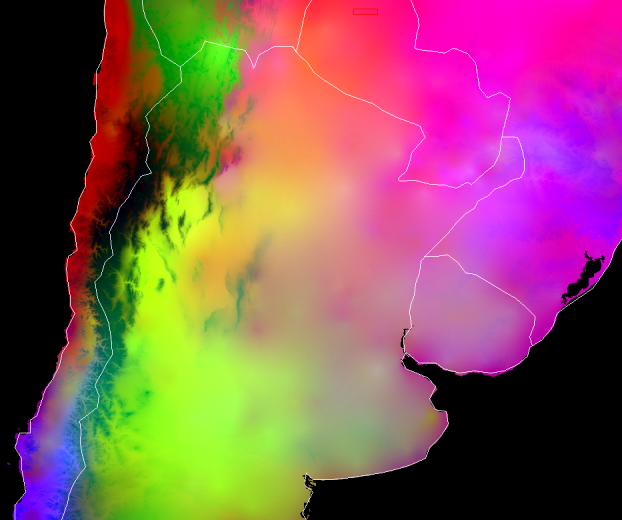
\includegraphics[width=0.6\textwidth]{images/temp_prec}%
      \caption{RGB: BIO1 = temperatura media anual, BIO7 = rango anual de
              temperatura (BIO5-BIO6) y BIO12 = precipitación anual, correspondientemente.}\label{fig:temp_prec}
    \end{figure}

    \begin{figure}[hbt]
      \centering%
      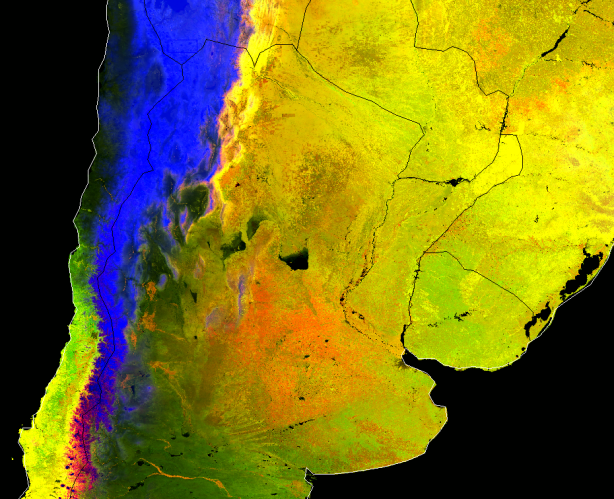
\includegraphics[width=0.6\textwidth]{images/ndvi_dem}%
      \caption{RGB: \textit{NDVI} de \textit{MODIS} promedio Enero, \textit{NDVI} de
               \textit{MODIS} promedio de Julio y DEM, correspondientemente.}\label{fig:ndvi_dem}
    \end{figure}

    \par De una manera similar, la Figura \ref{fig:ndvi_dem} presenta en RGB el
      \textit{NDVI} de \textit{MODIS} promedio de Enero, \textit{NDVI} de
      \textit{MODIS} promedio de Julio y el \textit{DEM}.

\section{Evaluación de la solución propuesta}

  \begin{figure}[hbt]

    \centering%
    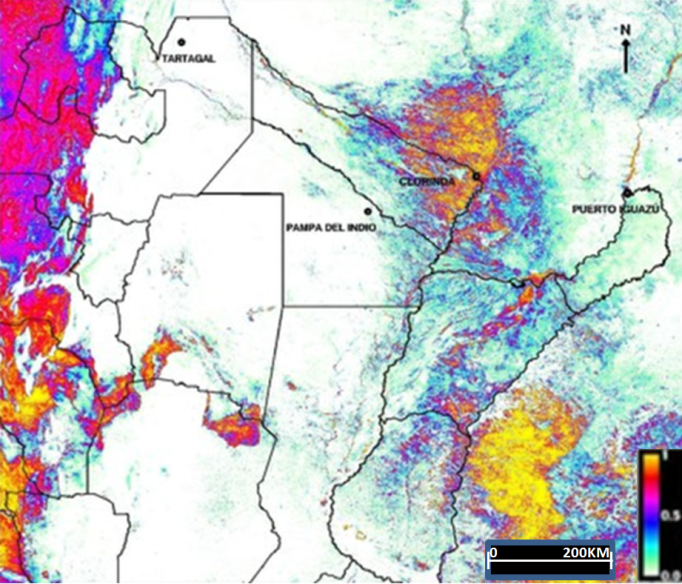
\includegraphics[width=0.6\textwidth]{images/ned_clorinda}%
    \caption{Similaridad ambiental ($\frac{1}{NED}$)
            de cada pixel a las condiciones de Clorinda}\label{fig:ned_clorinda}
  \end{figure}

  \begin{figure}[hbt]
    \centering%
    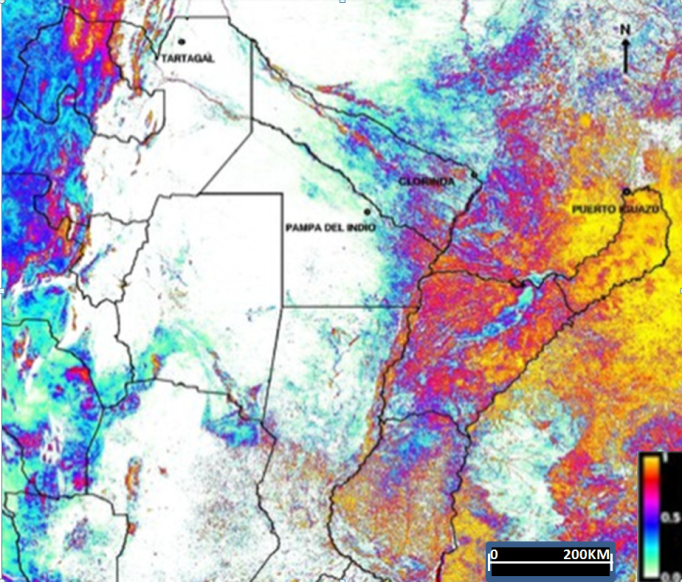
\includegraphics[width=0.6\textwidth]{images/ned_iguazu}%
    \caption{Similaridad ambiental ($\frac{1}{NED}$)
            de cada pixel a las condiciones de Iguazú}\label{fig:ned_iguazu}
  \end{figure}


  \par El resultado de las distancias ambientales normalizadas calculadas de
    cada pixel a cada una de las 4 ciudades se presenta en la Figuras
    \ref{fig:ned_clorinda}, \ref{fig:ned_iguazu}, \ref{fig:ned_pampa} y
    \ref{fig:ned_tartagal}. Es importante tener en cuenta que la inversa de Distancia Ambiental
    Normalizada ($\frac{1}{NED}$) nos dice qué tan similar es una ciudad en
    comparación con las otras tres.
    \begin{figure}[hbt]
      \centering%
      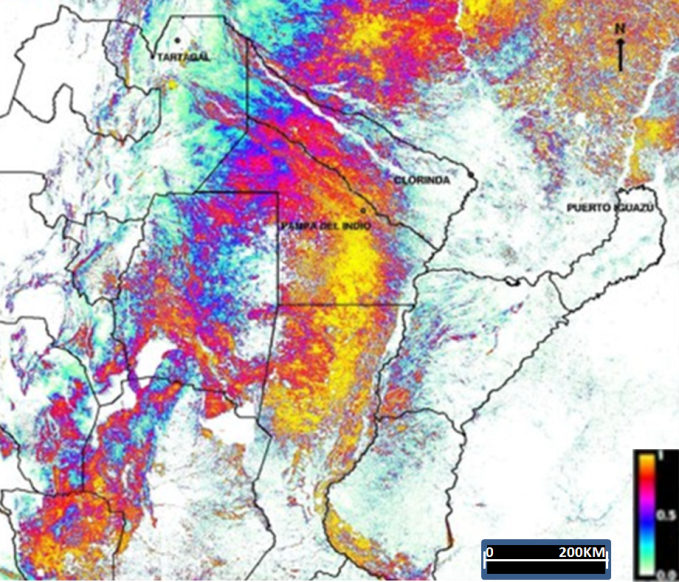
\includegraphics[width=0.6\textwidth]{images/ned_pampa}%
      \caption{Similaridad ambiental ($\frac{1}{NED}$)
              de cada pixel a las condiciones de Pampa del Indio}\label{fig:ned_pampa}
    \end{figure}


    \begin{figure}[hbt]
      \centering%
      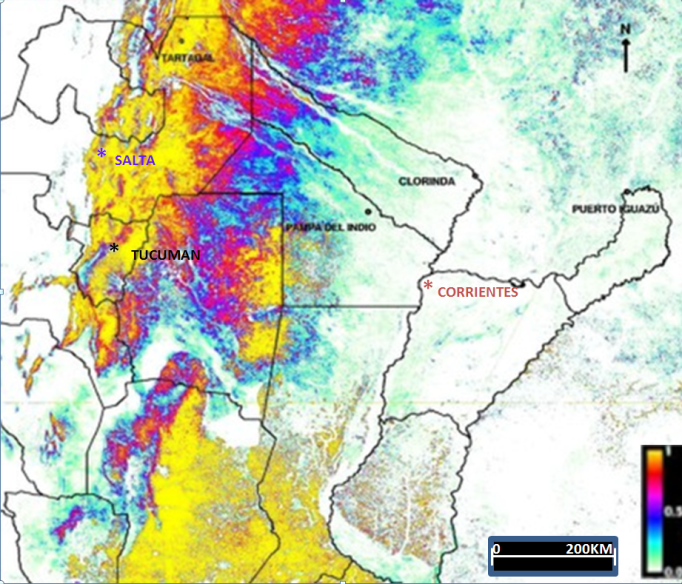
\includegraphics[width=0.6\textwidth]{images/ned_tartagal}%
      \caption{Similaridad ambiental ($\frac{1}{NED}$)
              de cada pixel a las condiciones de Tartagal.
              Aquí también se incluyen las localizaciones de las tres ciudades
              tomadas como ejemplo para el cálculo de nuevos modelos
              (Salta, Tucumán, Corrientes)}\label{fig:ned_tartagal}
    \end{figure}

  \par Claramente por estar normalizada, no es una medida de similaridad en
    términos absolutos. Así, por ejemplo en la Figura \ref{fig:ned_iguazu} los
    píxeles con valores
    cercanos a 1 significan que estos lugares son ambientalmente mucho más
    parecidos a Iguazú que a Tartagal o Clorinda o Pampa del Indio.


  \par Sólo como ejemplo, la inversa de la distancia normalizada ($\frac{1}{NED}$)
    de Tucumán, Corrientes y Salta se describen en la Tabla \ref{Tab:comparacion_ned}.
    Estos valores son presentados de una manera diferente en la Figura \ref{fig:ned_contrib}
    donde se intenta graficar con más claridad la contribución que tendrán cada
    uno de los 4 modelos previamente desarrollados, cuando se intenten modelar
    estas 3 nuevas ciudades.
    \begin{figure}[hbt][H]
      \centering%
      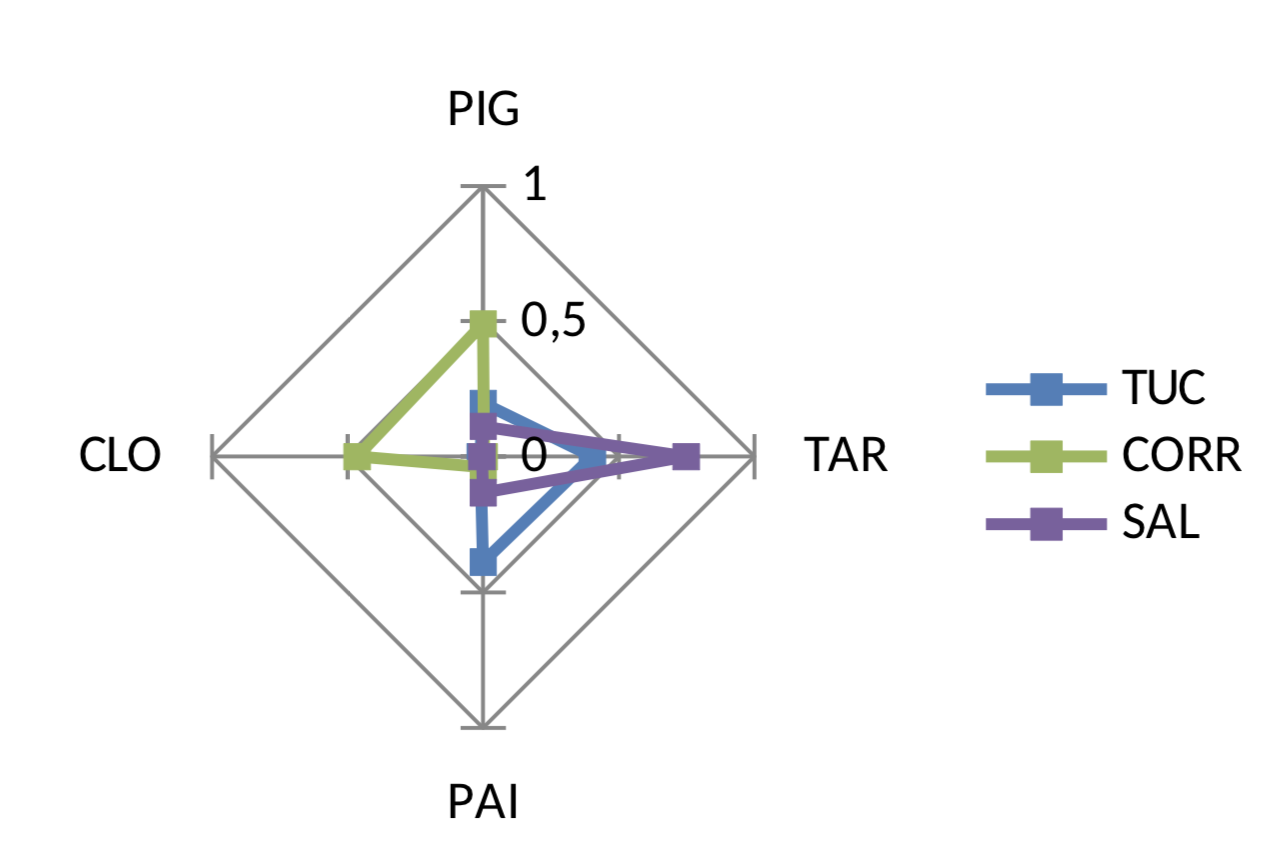
\includegraphics[width=0.6\textwidth]{images/ned_contrib}%
      \caption{Contribución que poseen los modelos para Salta, Corrientes y
              Tucumán de los 4 modelos disponibles}\label{fig:ned_contrib}
    \end{figure}

  \par Para el caso de las tres ciudades simuladas, la distancia ambiental
    realmente tiene una fuerte correlación con la distancia geográfica estándar.
    Estos ejemplos muestran más bien cómo el método funciona, que las ventajas
    que ofrece el mismo. Sin embargo la diferencia entre la distancia ambiental
    y la geográfica puede observarse claramente en las Figuras \ref{fig:ned_clorinda}
    a \ref{fig:ned_tartagal}.
    En todas ellas vemos cómo la distancia ambiental posee bordes abruptos
    (cosa que la distancia geográfica nunca tendrá).
    Por ejemplo en la Mesopotamia (Figura \ref{fig:ned_iguazu}) o en las yungas
    (Figura \ref{fig:ned_clorinda}) puede verse
    cómo pequeñas distancias geográficas tienen asociadas fuertes gradientes en
    la distancia ambiental (grandes distancias ambientales) y por ende
    podríamos suponer que localidades cercanas geográficamente poseen patrones
    temporales de la población de vectores muy diferentes.

    \begin{table}[hbt]
    \centering
    \caption{Inversa de NED de cuatro ciudades a las 4 localidades predefinidas}\label{Tab:comparacion_ned}
    \begin{tabular}{*7{r}}
    \toprule
    & Puerto Iguazú
    & Clorinda
    & Pampa del Indio
    & Tartagal \\ \midrule
    Tucuman
    &$0.197$
    &$0.011$
    &$0.388$%&\boldmath$1.108$  %CARO: cambio
    &$0.402$\\
    Corrientes
    &$0.491$
    &$0.466$
    &$0.039$
    &$0.002$ \\
    Salta
    &$0.112$
    &$0.005$
    &$0.133$   %CARO: cambio
    &$0.749$ \\
    \bottomrule
    \end{tabular}
    \end{table}

\section{Discusión y propuesta futura}
  \par En el presente capítulo pretendemos generar una contribución al objetivo de
    construir pronósticos dinámicos para la población de vectores,
    utilizando productos satelitales. Se aborda el problema de cómo generalizar
    espacialmente modelos ajustados para ciertas localidades específicas.

  \par Para ello, se propone una metodología basada en ideas ecológicas
    incorporando el concepto de distancia ambiental normalizada.
    Se ha mostrado que el mismo si bien es novedoso es conceptualmente simple.
    Se describe un método simple para calcularlo y ejemplos de su
    implementación especifica de la estimación de este parámetro en
    función de un conjunto de variables ambientales relevantes para la
    ecología del vector del dengue.

  \par Cabe resaltar que esta idea de interpolación ambiental que se
    plantea aquí para modelos relacionados a la epidemiologia,
    podría también ser utilizados a la hora de contar con datos
    puntuales de otras variables (por ejemplo rendimiento en la producción
    agrícola) donde la distancia espacial no refleje tan adecuadamente la
    similaridad entre sitios como lo es la distancia ambiental.


  \par Los resultados y metodologías aquí planteadas fueron presentadas en el
    \textit{Congreso Bienal de IEEE Argentina} (ARGENCON) durante la primer semana de Junio
    de 2018. La presentación fue realizada bajo el título
    \textit{Generalización espacial de modelos epidemiológicos basada en el
    concepto de Distancia Ambiental Normalizada NED} \cite{ned_scavuzzo} y
    se podrá encontrar en la \textit{IEEE Xplore Digital Library}\footnote{\url{https://ieeexplore.ieee.org/}}.
%\end{document}

%\documentclass[12pt,spanish,fleqn,openany,letterpaper,pagesize]{scrbook}

\usepackage[utf8]{inputenc}
\usepackage[spanish]{babel}
\usepackage{fancyhdr}
\usepackage{epsfig}
\usepackage{epic}
\usepackage{eepic}
\usepackage{amsmath}
\usepackage{threeparttable}
\usepackage{amscd}
\usepackage{here}
\usepackage{graphicx}
\usepackage{lscape}
\usepackage{tabularx}
\usepackage{subfigure}
\usepackage{longtable}


\usepackage{rotating} %Para rotar texto, objetos y tablas seite. No se ve en DVI solo en PS. Seite 328 Hundebuch
                        %se usa junto con \rotate, \sidewidestable ....


\renewcommand{\theequation}{\thechapter-\arabic{equation}}
\renewcommand{\thefigure}{\textbf{\thechapter-\arabic{figure}}}
\renewcommand{\thetable}{\textbf{\thechapter-\arabic{table}}}


\pagestyle{fancyplain}%\addtolength{\headwidth}{\marginparwidth}
\textheight22.5cm \topmargin0cm \textwidth16.5cm
\oddsidemargin0.5cm \evensidemargin-0.5cm%
\renewcommand{\chaptermark}[1]{\markboth{\thechapter\; #1}{}}
\renewcommand{\sectionmark}[1]{\markright{\thesection\; #1}}
\lhead[\fancyplain{}{\thepage}]{\fancyplain{}{\rightmark}}
\rhead[\fancyplain{}{\leftmark}]{\fancyplain{}{\thepage}}
\fancyfoot{}
\thispagestyle{fancy}%


\addtolength{\headwidth}{0cm}
\unitlength1mm %Define la unidad LE para Figuras
\mathindent0cm %Define la distancia de las formulas al texto,  fleqn las descentra
\marginparwidth0cm
\parindent0cm %Define la distancia de la primera linea de un parrafo a la margen

%Para tablas,  redefine el backschlash en tablas donde se define la posici\'{o}n del texto en las
%casillas (con \centering \raggedright o \raggedleft)
\newcommand{\PreserveBackslash}[1]{\let\temp=\\#1\let\\=\temp}
\let\PBS=\PreserveBackslash

%Espacio entre lineas
\renewcommand{\baselinestretch}{1.1}

%Neuer Befehl f\"{u}r die Tabelle Eigenschaften der Aktivkohlen
\newcommand{\arr}[1]{\raisebox{1.5ex}[0cm][0cm]{#1}}

%Neue Kommandos
\usepackage{Befehle}


%Trennungsliste
\hyphenation {Reaktor-ab-me-ssun-gen Gas-zu-sa-mmen-set-zung
Raum-gesch-win-dig-keit Durch-fluss Stick-stoff-gemisch
Ad-sorp-tions-tem-pe-ra-tur Klein-schmidt
Kohlen-stoff-Mole-kular-siebe Py-rolysat-aus-beu-te
Trans-port-vor-gan-ge}

%
%\begin{document}

\justifying

\chapter{Discusión y Conclusiones}

  \par Dengue, Chikungunya y Zika son enfermedades virales para las cuales no
    existen, al día de hoy, vacunas de prevención. Por lo tanto, el control
    más efectivo proviene de prevenir la propagación del mosquito
    \textit{Aedes Aegipty} (\textit{Linneaus}) y, por tanto, saber sobre la
    dinámica de su población es de suma importancia.

  \par Este trabajo, por un lado, presenta un \textit{framework} de simple
    utilización para el
    pronóstico de la oviposición utilizando
    únicamente variables ambientales extraídas de información satelital y
    herramientas de Aprendizaje Automático de libre acceso. Y por el otro,
    establece un concepto novedoso en el área de la epidemiología panorámica
    cuyo fin es lograr utilizar información de modelado de ciertos puntos grográficos
    para estimar la abundancia en muchos otros para los cuales no se posee
    información de campo. Este concepto es el de Distancia Ambiental Normalizada.

  \par Las herramientas implementadas en el \textit{framework}
    son una mejora al sistema operacional de riesgo de
    Argentina \cite{porcasi_operative}. A su vez, por la arquitectura del mismo,
    es posible agregar modelos nuevos y modificar las variables independientes a utilizar como
    predictores (\textit{features}) de una manera sencilla.

  \par En este caso, se utilizaron variables ambientales derivadas de información satelital
    (temperatura, humedad y precipitación) operacionalmente disponibles para
    construir modelos temporales capaces de predecir la actividad de oviposición
    fuera de las casas. En ese sentido, la perspectiva planteada, completamente operativa,
    implica generar un procedimiento para estimar la actividad del vector
    y eventualmente independizarse de las mediciones de campo. Dicha contribución
    se considera de alto valor, entre otras cosas, porque realizar la medición
    de oviposición en 50 casas todas las semanas, durante
    largos períodos de tiempo (como se utilizó para generar los modelos) tiene
    un costo extremádamente alto.

  \par Este estudio resulta ser un avance sobre trabajos previos en el área
    de la epidemiología panorámica, donde se consideran modelos estadíticos utilizando
    relaciones lineales \cite{models_predicting, modis_data, ndwi_erffectiveness}
    en terminos de la capacidad predictiva de los modelos desarrollados aquí.
    Estas mejoras fueron obtenidas utilizando herramientas de Aprendizaje
    Automático que, en este caso, no requieren de un esfuerzo adicional de
    parte del usuario.

  \par La metodologia implementada muestra que algunas herramientas \textit{out-of-the-shelf}
    son capaces de manejar las complejas relaciones entre variables, proporcionando
    así una forma de abordar este importante problema. Este enfoque interdisciplinario
    proporciona nuevas herramientas para los profesionales que se encuentran
    trabajando en esta área.

  \par A su vez, este trabajo es un ejemplo de cómo el uso de herramientas
    automáticas para la configuración de algoritmos, como \textit{iRace} pueden
    reducir la complejidad del ajuste de hiperparámetros de los modelos y
    proveer un marco de referencia para la selección de los mismos.
    Adicionalmente, se muestra la importancia de la utilización de la Validación
    Cruzada (VC), raramente utilizada en usuarios del Sensado Remoto.
    Utilizamos VC para disminuir la dependencia de los resultados de evaluación
    sobre una selección particular de los conjuntos de entrenamiento y validacíon
    en la etapa de elección del modelo. Aqui se Utiliza
    un procedimiento particular de CV para series de tiempo. Todos los modelos
    aquí discutidos pueden ser ejecutados con \textit{scripts} de Python
    disponibles libres en \url{https://github.com/juansca/modeling-mosquitos}.

  \par En lo que respecta a la comparacion de algoritmos, se encontró que la Regresión
    por K-Vecinos Cercanos (KNNR), el Perceptron Multicapa (MLP) y la
    \textit{Support Vector Machine} resultan ser los modelos predictivos de la
    población de vectores que mejores resultados arrojan.


  \par A pesar de que el período utilizado es largo en comparación con trabajos similares
    sobre poblaciones del vector, el desempeño de estos algoritmos puede ser
    mejorado sustancialmente utilizando conjuntos de datos más grandes.
    Otra manera de mejorarlos seria realizar ajustes más finos en el modelado
    y/o bien utilizar otras técnicas de mayor complejidad dentro del área del
    Aprendizaje Automático.

  \par La otra importante contribución de este trabajo está relacionada con la
    necesidad de poseer modelos de oviposición para distintas ciudades, evitando
    el gran costo de la recolección de datos y el entrenamiento para cada una de
    las ciudades o puntos para los cuales se quiera poseer datos. Aquí presentamos
    una forma de establecer relaciones entre los distintos lugares geográficos teniendo
    en cuenta las características ambientales que poseen. La hipótesis más fuerte que
    asumimos es la que nos dice que el comportamiento de los vectores está altamente
    correlacionado (al menos dentro de cierto rango) a las características ambientales
    del punto en el que que se observa.

  \par Asi se presenta, desarrolla e implementa el concepto de Distancia Ambiental
    Normalizada, el cual permite
    llevar a cabo lo mencionado en el párrafo anterior estableciendo una distancia
    vectorial utilizando el espacio de características ambientales extraídas de
    información satelital, en vez del espacio geográfico.

  \par En conjunto, ambas contribuciones aportan un muy alto valor de capacidad de
    mejora al sistema operacional de riesgo de la república Argentina. A su vez,
    en perspectiva, aporta valor a la proyección de mejora de dichos modelos por
    su facilidad de uso y extrapolación a distintas zonas.

  \par Otro punto de valor del trabajo es el caracter integrador e
    interdisciplinario del mismo, demostrando la utilidad y la necesidad
    de la incersión del Aprendizaje Automático en áreas de impacto social.

  \par A su vez, cabe destacar que lo desarrollado involucra conocimientos de
    diversas áreas de las Ciencias de la Computación abarcando temáticas, por ejemplo, de
    Ingeniería del Software, a la hora de realizar el análisis de requerimientos,
    generación de la arquitectura y establecer la metodología de trabajo.
    Por otra parte, también se utilizan conocimientos de estadística, modelos y
    simulación y distintas áreas de matemática para el entendimiento de los
    distintos algoritmos, tomar decisiones con respecto a
    ellos y a las hipótesis y conclusiones. Muchos otros conceptos aprendidos
    a nivel general por las distintas materias han sido aplicados en el desarrollo.
    Es por esto que me resulta de suma importancia mencionar que lo realizado en
    este trabajo, con las características interdisciplinarias y la envergadura
    del mismo, me permitió integrar, de una manera muy contructiva para mi
    desarrollo profesional, todo lo aprendido y adquirido a lo largo de la carrera.

  \par Es importante resaltar finalmente que los resultados y metodologías
    incluidos en este trabajo de grado han dado lugar a tres publicaciones
    indexadas en la base de datos scopus, a saber:

    \begin{itemize}
      \item pooooner las ciiitas
    \end{itemize}
    \textit{Modeling Dengue Vector Population Using Remotely Sensed Data and
    Machine Learning} \cite{scavuzzo2018modeling} y
    \textit{Generalización espacial de modelos epidemiológicos basada en el
    concepto de Distancia Ambiental Normalizada NED} en
    en la revista \textit{Acta Tropica}
    de \textit{Elsevier} (\url{https://www.journals.elsevier.com/acta-tropica})
    y \textit{IEEE Xplore Digital Library} (\url{https://ieeexplore.ieee.org/})
    correspondientemente.
%\end{document}

%\chapter{Conclusiones y recomendaciones}
\section{Conclusiones}
Las conclusiones constituyen un cap\'{\i}tulo independiente y presentan, en forma l\'{o}gica, los resultados de la tesis  o trabajo de investigaci\'{o}n. Las conclusiones deben ser la respuesta a los objetivos o prop\'{o}sitos planteados. Se deben titular con la palabra conclusiones en el mismo formato de los t\'{\i}tulos de los cap\'{\i}tulos anteriores (T\'{\i}tulos primer nivel), precedida por el numeral correspondiente (seg\'{u}n la presente plantilla).\\

\section{Recomendaciones}
Se presentan como una serie de aspectos que se podr\'{\i}an realizar en un futuro para emprender investigaciones similares o fortalecer la investigaci\'{o}n realizada. Deben contemplar las perspectivas de la investigaci\'{o}n, las cuales son sugerencias, proyecciones o alternativas que se presentan para modificar, cambiar o incidir sobre una situaci\'{o}n espec\'{\i}fica o una problem\'{a}tica encontrada. Pueden presentarse como un texto con caracter\'{\i}sticas argumentativas, resultado de una reflexi\'{o}n acerca de la tesis o trabajo de investigaci\'{o}n.\\
%\begin{appendix}
\chapter{Anexo: Detalles del código}\label{Anexo_codigo}

  \par Se decidió realizar todo el desarrollo en el lenguaje de programación
    \textit{Python} por su simplicidad, buen desempeño y su extensa
    comunidad activa. Esto facilita el desarrollo, incrementa la velocidad
    de producción y, como un factor muy importante, también permite
    una usabilidad amena de usuario final. El proyecto está disponible
    en \url{https://github.com/juansca/modeling-mosquitos} y en su sección
    inicial se pueden encontrar instrucciones para su instalación.
    A continuación se describirán
    algunos detalles que se consideran importante de los distintos módulos,
    sin entrar en cuestiones irrelevantes.

  \par El módulo \verb|data| por un lado tiene un archivo llamado
    \verb|constants.py| en donde se definen algunas constantes que
    son dependientes del conjunto de datos que se utilizará. Es importante
    dado que es allí en donde se especifican los \textit{features} (o
    columnas) que se utilizarán como input para predicción.
    A su vez, en dicho módulo, el archivo \verb|data_cleaner.py|
    posee una clase llamada \verb|DataCleaner| que es la encargada de
    realizar la limpieza de los datos. Para realizar la limpieza de los
    datos se debe ejecutar el script \verb|scripts/clean_data.py|, el
    cual arroja el siguiente instructivo:

    \begin{lstlisting}
    $ python data/scripts/clean_data.py --help

    Clean Data.

    Usage:
      ./clean_data.py -i <file> -o <dir> [--p_eval <float>] [--instances <n>] [--overlap <f>]

    Options:
      -i <file>              Evaluate dataset path
      -o <dir>               Directory where the evaluation plot result will be
                             saved
      --p_eval <float>       Percentage to evaluation dataset. [default: 0.2]
      --instances <n>        Number of instances to generate from data
                             [default: 1]
      --overlap <f>          Percentage of overlapping between the instances.
                             [default: 0]

    \end{lstlisting}


  \par Por otro lado, el módulo \verb|models| tiene un archivo llamado
    \verb|models.py| en el cual se declaran los modelos
    que se utilizarán para el modelado. Es importante que estos modelos
    sigan la estructura ahí utilizada para que los demás módulos los
    puedan utilizar correctamente.

  \par Además, allí se encuentra el \textit{script} de entrenamiento,
    \verb|scripts/train.py|, que entrena el modelo elegido con el conjunto
    de datos dado e imprime por linea de comandos un conjunto de
    estadísticas que resultan de realizar validación cruzada sobre
    los datos brindados por el usuario para dicha tarea. Ésto resulta útil
    para tener una noción del desempeño del modelo.
    Éste script devuelve la siguiente documentación de uso:
    \begin{lstlisting}
    $ python models/scripts/train.py --help

    Train a model

    Usage:
      ./train.py -i <file> --model <model> [-p <file>]
      ./train.py -h | --help

    Options:
      -i <file>         Train/Val dataset path
      --model <model>   Model you want to train, is mandatory that it was on
                        models.py file.
      -p <file>         CSV file where are saved the hyperparameters
                        (in case of tunning module was used).
    \end{lstlisting}

  \par Por otra parte, el módulo posee un \textit{script} de evaluación,
  que, además de imprimir por linea de comandos el valor del Error Cuadrático Medio de la
  evaluación, genera un gráfico con la curva real y la curva predicha
  por el modelo y lo guarda en un directorio. A su vez, guarda un
  archivo \verb|csv| con los valores reales y los generados por el modelo
  facilitando así, la posterior manipulación del mismo.
  La documentación de ayuda para su utilización es:
  \begin{lstlisting}
  $ python models/scripts/eval.py --help

  Evaluate a model

  Usage:
    ./eval.py -i <file> -m <model> [-o <file>]

  Options:
    -i <file>         Evaluate dataset path
    -m <model>        Model you want to evaluate as pickle format
    -o <dir>          Directory where the evaluation plot result will be saved

  \end{lstlisting}

\par Finalmente, el sistema desarrollado posee el módulo \verb|tunning|.
  Allí se realiza el ajuste de hiperparámetros de los modelos.
  Existe varios archivos en ese módulo que son los que hacen de interfaz
  con la herramienta \textit{irace}. Algo que cabe destacar aquí es el
  directorio \verb|parameters|. Allí se colocan los posibles
  (o intervalos de) valores que generan el espacio de hiperparámetros
  donde la herramienta buscará los óptimos para cada modelo. Además,
  \textit{irace}, usará las instancias de datos en \verb|instances|
  para realizar dicha tarea. Algo de suma importancia es que
  los datos utilizados para generar los últimos conjutos deben ser distintos
  a los que se usarán posteriormente en el entrenamiento o validación de
  los modelos. Esto se debe a que si no, se puede generar una dependencia
  de los datos y podría llevar al sobre-ajuste (\textit{overfitting})\footnote{Una
  analogía clara es que el modelo aprende "de memoria" los datos en vez de
  comprenderlos. Esto lleva a una muy pobre capacidad de generalización.}.
  El \textit{script} que se debe ejecutar para hacerlo es \verb|tune_params.py|.
  Su documentación de uso es:
  \begin{lstlisting}
  $ python tunning/tune_params.py --help

  Tune parameters for given models.

  Usage:
    tune_params.py --model <name>

  Options:
    --model <name>           model name to tune params.
                             Options: svr, rdmforest, pcardmforest, dtr, knnr,
                             mlpr, svr, pcaknnr, pcadtr.
                             If you want to tune all the models together, just
                             put on this parameter 'all'.
    --help                   show this screen

  \end{lstlisting}
\par Por último, en la Figura \ref{fig:proyecto_modelado} se puede observar
  la estructura general del proyecto.

  \begin{figure}[hbt]
  \centering%
  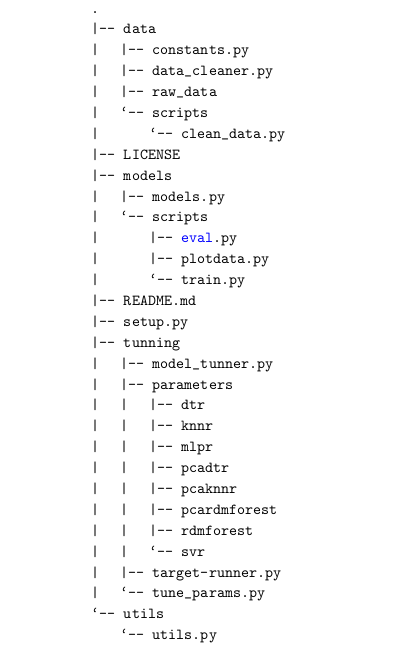
\includegraphics[width=0.6\textwidth]{images/proyecto_modeling}%
  \caption{Sistema para el ajuste de parámetros y modelado}\label{fig:proyecto_modelado}
  \end{figure}

\end{appendix}

\addcontentsline{toc}{chapter}{\numberline{}Bibliografía}
\bibliographystyle{abbrv}
\bibliography{mainTesis}
\end{document}
